\documentclass[12pt]{article}
\usepackage[margin=0.75in]{geometry}

%%%%%%%%%%%%%%%%%%%%%%%%%%%%%%%%%%%%%%%%%%%%%%%%%%%%%%%%%%%%%%%%%%%%%%%%
%                                                                      %
%               LATEX COMMANDS FOR DOCUMENT SETUP                      %
%                                                                      %
%%%%%%%%%%%%%%%%%%%%%%%%%%%%%%%%%%%%%%%%%%%%%%%%%%%%%%%%%%%%%%%%%%%%%%%%

\usepackage{lmodern}
\usepackage[us,nodayofweek,12hr]{datetime}
\usepackage{graphicx}
\usepackage{rotating}
\usepackage{subfigure}
\usepackage[none]{hyphenat}
\emergencystretch 3em
\usepackage[hyphens]{url}
\usepackage{hyperref}
\usepackage{amsmath}
\usepackage{enumitem}
\usepackage[capitalize]{cleveref}
\usepackage{multirow}
\usepackage{comment}
\usepackage{amsfonts}
\usepackage{courier}
\usepackage{amssymb}
\usepackage{rotating}
\usepackage{afterpage}
\usepackage{mathtools}
\usepackage{xcolor}
\newcommand{\mb}[1]{\mathbf{#1}}
\newcommand{\mc}[1]{\mathcal{#1}}
\newcommand\blankpage{%
    \null
    \thispagestyle{empty}%
    \addtocounter{page}{-1}%
    \newpage}
\usepackage{caption}
\captionsetup[figure]{labelfont={bf},name={Fig.},labelsep=period}
\captionsetup[table]{labelfont={bf},name={Table},labelsep=period}

% HERE
\usepackage[english]{babel}
\usepackage{csquotes}
\usepackage[backend=biber, bibstyle=ieee]{biblatex}
\renewbibmacro{in:}{}
\addbibresource{references.bib}
\let\cite\parencite
% HERE

\hypersetup{%2
    pdfborder = {0 0 0}
}
\usepackage{bm}
\usepackage[parfill]{parskip}

\newcommand*{\figref}[2][]{%
  \hyperref[{fig:#2}]{%
    {Fig.~\ref*{fig:#2}}%
    \ifx\\#1\\%
    \else
      \,#1%
    \fi
  }%
}

\newcommand*{\tabref}[2][]{%
  \hyperref[{tab:#2}]{%
    {Table~\ref*{tab:#2}}%
    \ifx\\#1\\%
    \else
      \,#1%
    \fi
  }%
}

\newcommand*{\eqnref}[2][]{%
  \hyperref[{eqn:#2}]{%
    {Equation~\ref*{eqn:#2}}%
    \ifx\\#1\\%
    \else
      \,#1%
    \fi
  }%
}

\newcommand*{\chapref}[2][]{%
  \hyperref[{chap:#2}]{%
    {Chapter~\ref*{chap:#2}}%
    \ifx\\#1\\%
    \else
      \,#1%
    \fi
  }%
}

\usepackage{accents}
\newlength{\dhatheight}
\newcommand{\doublehat}[1]{%
    \settoheight{\dhatheight}{\ensuremath{\hat{#1}}}%
    \addtolength{\dhatheight}{-0.35ex}%
    \hat{\vphantom{\rule{1pt}{\dhatheight}}%
    \smash{\hat{#1}}}}
        
\DeclareMathAlphabet\mathbfcal{OMS}{cmsy}{b}{n}   

\hyphenation{dis-ser-ta-tion blue-print man-u-script pre-par-ing}

\setlength{\parindent}{0pt}

%\usepackage{bookmark}
%\usepackage[us,nodayofweek,12hr]{datetime}
%\usepackage{graphicx}

%\usepackage{fullpage}
%\usepackage{graphicx}
%\usepackage{tabularx}
%\usepackage{multirow}
%\usepackage{subfigure}
%\usepackage{wrapfig}
%\usepackage{textcomp}
%\usepackage[square, comma, numbers, sort&compress]{natbib}
%\usepackage[hang,small,bf]{caption}
%\usepackage{parskip}
%\usepackage[margin=1in,footskip=0.5in]{geometry}
%\usepackage{amsmath}
%\usepackage{mdwlist}
%\usepackage{epstopdf}
%\usepackage[section]{placeins}

%\newcommand{\para}{\vspace{5mm} \noindent}
%\newcommand{\parafig}{\vspace{4mm} \noindent}
%\newcommand{\paraeq}{\vspace{1mm} \noindent}
%\newcommand{\negparafig}{\vspace{-4mm} \noindent}
%\newcommand{\negparaeq}{\vspace{-1mm} \noindent}

%\addtolength{\parskip}{1\parskip}

%\bibliographystyle{plain}
%\bibliographystyle{ieeetr}
%many other bibliography styles are available (IEEEtran, mla, etc.). Use one appropriate for your field.

%\hyphenation{pre-par-ing} %add hyphenation rules for words TeX doesn't know

%\usepackage[square,comma,numbers,sort&compress]{natbib}
%\usepackage{hypernat}
% Other useful packages to try
%\usepackage{amsmath}
%\usepackage{amssymb}
%\usepackage{accents}

%\usepackage{setspace}
%\usepackage{algorithm}
%\usepackage{algorithmic}
%
% Different fonts to try (uncomment only fontenc and one font at a time)
% (you may need to install these first)
%\usepackage[T1]{fontenc} %enable fontenc package if using one of the fonts below
%\usepackage[adobe-utopia]{mathdesign}
%\usepackage{tgschola}
%\usepackage{tgbonum}
%\usepackage{tgpagella}
%\usepackage{tgtermes}
%\usepackage{fourier}
%\usepackage{fouriernc}
%\usepackage{kmath,kerkis}
%\usepackage{kpfonts}
%\usepackage[urw-garamond]{mathdesign}
%\usepackage[bitstream-charter]{mathdesign}
%\usepackage[sc]{mathpazo}
%\usepackage{mathptmx}
%\usepackage[varg]{txfonts}


%%%%%%%%%%%%%%%%%%%%%%%%%%%%%%%%%%%%%%%%%%%%%%%%%%%%%%%%%%%%%%%%%%%%%%%%
%                                                                      %
%        DOCUMENT SETUP AND INFORMATION FOR PRELIMINARY PAGES          %
%                                                                      %
%%%%%%%%%%%%%%%%%%%%%%%%%%%%%%%%%%%%%%%%%%%%%%%%%%%%%%%%%%%%%%%%%%%%%%%%

\begin{document}

%%%%%%%%%%%%%%%%%%%%%%%%%%%%%%%%%%%%%%%%%%%%%%%%%%%%%%%%%%%%%%%%%%%%%%%%

\vspace{7cm}
\begin{center}
	{\bf\Large \textcolor{purple}{A robust workflow for b-rep generation from image masks}}
\end{center}

\vspace{1cm}
\begin{center} 
	{\bf\large Omar M Hafez}{\bf\large, Mark M Rashid}\\
	
	%\vspace{5mm}
	{Department of Civil \& Environmental Engineering, University of California, Davis}\\
\end{center}

\vspace{1cm}
\abstract{\noindent A novel approach to generating closed, manifold, watertight boundary representations from binary image masks of MRI or CT scans is presented. The method samples an input segmented image and locally approximates the material boundary. Geometric error metrics between the voxelated boundary and an approximating template surface are minimized, and boundary point/normals are correspondingly generated. Voronoi partitioning is employed to perform surface reconstruction on the resulting oriented point cloud. The method performs competitively compared to commercial software, both in honoring shape and volume metrics of an underlying canonical image mask, as well as in a qualitative comparison using examples from real scans. The approach provides robust, high-quality data that may be inserted into an image-based meshing pipeline for physics-based simulation, 3D printing, or visualization applications. The framework readily admits enhancements in the form of additional interface templates for purposes of capturing sharp edges and corners, high-curvature regions, and multi-material interfaces.} \\ \\
{\bf Keywords:} surface generation, b-rep generation, surface reconstruction, Voronoi partitioning, image-based meshing, image-based modeling, physics-based simulation, finite element analysis, 3D printing, visualization

%%%%%%%%%%%%%%%%%%%%%%%%%%%%%%%%%%%%%%%%%%%%%%%%%%%%%%%%%%%%%%%%%%%%%%%%

% Each chapter can be in its own file for easier editing and brought in with the \include command.
% Then use the \includeonly command to speed compilation when working on a particular chapter.
%%% \includeonly{chap1}

%\newcommand{\bibfont}{\singlespacing}
% need this command to keep single spacing in the bibliography when using natbib

% HERE
% \bibliographystyle{ieeetr}
% HERE

\section{Introduction}

Image-based modeling and simulation is becoming an increasingly important analytic and predictive tool for a variety of medical and engineering applications. Some examples include patient-specific diagnosis and treatment, large-scale \textit{in silico} trials, medical device design, computer-assisted surgery, and as-built analysis of existing parts. Whereas traditional physics-based modeling and simulation typically uses NURBS-based surfaces generated from CAD software to define geometries of interest, the image-based analog extracts geometries from imaging data, typically in the form MRI or CT. The field of image-based modeling and simulation covers a broad spectrum of topics, including image processing, computational geometry, numerical methods, and continuum mechanics. The workflow entails: image acquisition, image segmentation, image-based mesh generation, and finally the application of interest. This paper focuses on one component of the image-based meshing step, namely: surface generation. The other steps are briefly mentioned below, but otherwise the focus shall remain on surface generation from a segmented image. \\ \\
%
Medical imaging is the process of generating discrete image representations of the regions of interest. For our purposes, the acquired image provides a three-dimensional rectilinear grid of point intensity values as input to the rest of the workflow. In the case of MRI, those values are weighted proton densities, which effectively measure water-content. In the case of CT, they are attenuation measurements from an x-ray beam source, which effectively measure density. For typical applications, we can expect millimeter resolution, and in some cases even better~\cite{van2012super}.\\ \\
%
Image segmentation is the process of partitioning an image into non-overlapping regions corresponding to different tissues or objects in an image. Contrast differences between neighboring tissues can be difficult to identify due in part to noise and artifacts, and thus image processing in the form of smoothing, filtering, and resampling are performed to improve the effectiveness of the image segmentation technique. The output from image segmentation consists of one or more \textit{image masks}, depending on how many regions of interest exist in the field of view. If there is only one region of interest, the output is termed a \textit{binary image mask}. A few popular techniques in image segmentation include simple thresholding, level set methods~\cite{malladi_1995, sethian_1996}, machine learning-based approaches~\cite{litjens_2017}, and often in practical cases, manual fine-tuning.\\ \\
%
Image-based meshing is the process of generating explicitly defined volume meshes from imaging data. For our purposes, we focus on generating meshes specifically from segmented image data. The challenge is to define the mesh explicitly in terms of vertex coordinates, corresponding polytopes, and the connectivity of those polytopes, as opposed to an implicit definition of the volume enclosed by the zero-set of a 4D indicator function. Image-based meshing is often separated into two steps: 1) surface generation, and 2) conventional CAD-based volume meshing. Surface generation (or surface extraction) is a matter of generating a watertight, manifold \textit{boundary representation} (or \textit{b-rep}). B-reps may refer to polygonized surface meshes or NURBS surfaces; for our purposes we will restrict the scope to surface meshes. \\ \\
%
Various approaches have been pursued to tackle image-based meshing, most of which are extensions of the \textit{marching cubes} algorithm~\cite{lorensen_1987}. It assumes an implicit isosurface exists whose associated volume is the union of voxels in an image mask that belong to the same region. Triangular patches are generated to approximate the intersection of this isosurface with each grid cell and are combined to form a continuous surface. The two most glaring limitations of the marching cubes algorithm are that 1) the resulting surfaces exhibit aliasing artifacts that poorly capture smooth and sharp features alike, and 2) the algorithm is limited to surface generation from binary masks (i.e., it cannot generate surfaces for multi-material masks). Advances in the field of image-based meshing have mostly focused on modifications to the marching cubes algorithm to address these two limitations - namely, 1) generating smooth surfaces that represent the original object accurately while preserving sharp features; and 2) generating quality surface meshes for general multi-material image masks. \\ \\ 
%
Updegrove \textit{et al.}~\cite{updegrove_2016} used a \textit{lofting} technique on a series of 2D segmentations to generate models of blood vessels. An approximate centerline must be drawn, and 2D segmentations are combined using spline interpolating functions to generate surfaces. Unstructured tetrahedral meshes are then generated from the surfaces. Lofting is known as a 2.5D approach because stacking contours of neighboring slices cannot capture arbitrary 3D topologies. The approach often suffers from significant loss of accuracy, and the interpolating splines typically require manual selection of control points~\cite{young_2008}. Treating an image mask as a series of 2D masks was a popular approach in past decades, but most modern approaches treat it as a three-dimensional object to avoid the drawbacks of lofting techniques. \\ \\
%
Young \textit{et al.}~\cite{young_2008} used a \textit{direct meshing} approach to generate meshes from multi-material image masks without the intermediate step of creating a surface mesh. Young \textit{et al.} combined the surface generation and mesh generation stages into one process via their \textit{enhanced volumetric marching cubes} approach. Standard volumetric marching cubes generates tetrahedral volumes from the intersection of the isosurface with grid cells, rather than just triangular surface patches. The authors extended the volumetric algorithm to handle intersections of up to eight regions in one grid cell - the maximum number of intersections that can occur for a Cartesian grid. The resulting mesh is \textit{mixed hex-tet}, where tetrahedra exist near the surface based on the extended volumetric marching cubes approach; internal voxels are converted directly to hexahedra; and pyramidal and tetrahedral elements exist in the transitional layer in between. The authors also utilized partial volume-based interpolation to improve surface smoothness. Additional efforts to reduce the mesh size were made by converting surface tetrahedra to hexahedra where appropriate, and by performing an octree-based approach to collect neighboring interior hexahedral elements into larger elements. Nonetheless, this \textit{grid-based} approach results in a surface mesh that is very fine, which subsequently constrains the size of interior elements in the volume mesh. The resulting mesh from this approach yields an intractably large number of degrees of freedom for simulation purposes. Thus, for practical purposes, the number of points and polyhedra defining the surface must be reduced (or \textit{decimated}), to allow for a subsequent coarser volumetric discretization. Indeed, the default and recommended approach in their software \textit{Simpleware} (known as \textit{+FE Free}) is to follow the two-step paradigm of surface generation followed by CAD-based meshing as described previously. Namely, the software extracts the resulting surface following the extended volumetric marching cubes step, performs multi-part decimation and smoothing~\cite{egst}, and finally uses a conventional CAD-based tetrahedral mesher to generate fully tetrahedral meshes from the polygonized surfaces. \\ \\
%
Meyer \textit{et al.}~\cite{meyer_2008} employed a \textit{particle-based sampling} technique for multi-material volumes. Surface samples (called \textit{particles}) are constrained to the zero-set of an implicit function. The distances between particles are locally adapted to create higher densities of points near surface features. A Delaunay tetrahedralization of the sampling points is computed, and each tetrahedron is assigned a material label. The surface mesh is generated by extracting the faces bounded by tetrahedra with different material labels. Finally, a conventional CAD-based tetrahedral mesher is once again employed to produce an analysis-ready mesh. The approach faithfully and robustly captures the geometries of complex material interfaces, but has debilitating performance issues, even by the own admission of the authors. \\ \\
%
A number of other techniques have been published on the topic of image-based meshing, often attacking the problem from completely different perspectives~\cite{fang_2009, mohamed_2004, jermyn_2013, boissonnat_2009}. Although several of the works presented here attempt to generate surfaces for multi-material image masks, a great deal of effort and applicability still exists for generating high-quality surfaces (and resulting meshes) from binary image masks. This will be the focus of the paper, as we propose a novel Voronoi-based surface generation approach that guarantees watertightness and lays out a framework that has the potential to ultimately reconstruct a wider array of boundaries, including those with sharp edges or corners. The method is also simple to use, freeing the user from a complicated set of parameters that need to be modified for optimal results. \\ \\
%
Provided a triangulated surface mesh from any of the aforementioned approaches, conventional CAD-based volume-meshing techniques are utilized to produce a final volume mesh. Since a general automatic hexahedral meshing algorithm has yet to be developed, tetrahedral meshing is usually the method of choice for arbitrary input surfaces. The two most widely adopted approaches for automated unstructured tetrahedral mesh generation are \textit{advancing front}~\cite{jin_1993, lohner_1988} and \textit{Delaunay tetrahedralization}~\cite{lohner_1997}. \\ \\
%
Finally, applications for this work range from 3D printing to visualization to finite element analysis (FEA). In the case of 3D printing and visualization, b-reps can be used for surgery planning, custom surgical guides and implants, rapid prototyping, and generation of CAD surfaces from existing parts. Meanwhile, image-based simulation has been performed on nearly every major organ in the body and shows great promise in advancing both personalized medicine~\cite{neal2010current} and large-scale clinical trials~\cite{viceconti2016silico}. In addition, image-based simulation offers the ability to perform non-destructive analysis on as-built engineering parts or legacy parts whose CAD may not be available~\cite{bradley2005advances}.\\ \\
%
Given the context of the image-based modeling and simulation workflow within which it fits, the novel Voronoi-based surface generation method is now proposed herein. The algorithm is followed by a performance assessment in comparison to a state-of-the-art commercial software, which are made for a variety of canonical cases as well as for cases from real MRI and CT data. The paper is closed with a summary and discussion of future directions for this work.

\section{\textcolor{purple}{Proposed Workflow}}

The details of our approach are presented in this section.  In the subsections that follow, the three main elements -- generation of an oriented point cloud, Voronoi-based surface reconstruction, and decimation/smoothing -- are treated individually.  We confine attention to the single-material case, i.e. a binary image mask, and take the image mask as our starting point.  Given a segmented image, we seek to generate a b-rep for the region occupied by the material, i.e. the solid body.  This b-rep takes the form of one or more watertight collections of polygonal facets.

\subsection{Point-Cloud Generation}
\label{Point Cloud Generation}

A point cloud is ``oriented'' if unit surface normals are computed at each point in addition to the point's spatial coordinates. The algorithm computes the point cloud by sampling the image mask with small, overlapping \textit{windows} to locally approximate the material boundary. For each three-dimensional window, the following tasks are performed:
\vspace{2mm}
\begin{itemize}[noitemsep]
  \item Predict whether the window intersects the material boundary.
  \item Locally approximate the boundary via an optimization problem. 
  \item Place a point and associated normal on the approximated boundary surface.
\end{itemize}
\vspace{2mm}
The basic sequence is shown in 2D in panels (a-c) of \figref{vor}. Each step in generating oriented point clouds is detailed in the subsections below.

\begin{figure}[ht]
\centering
\subfigure[]{%
		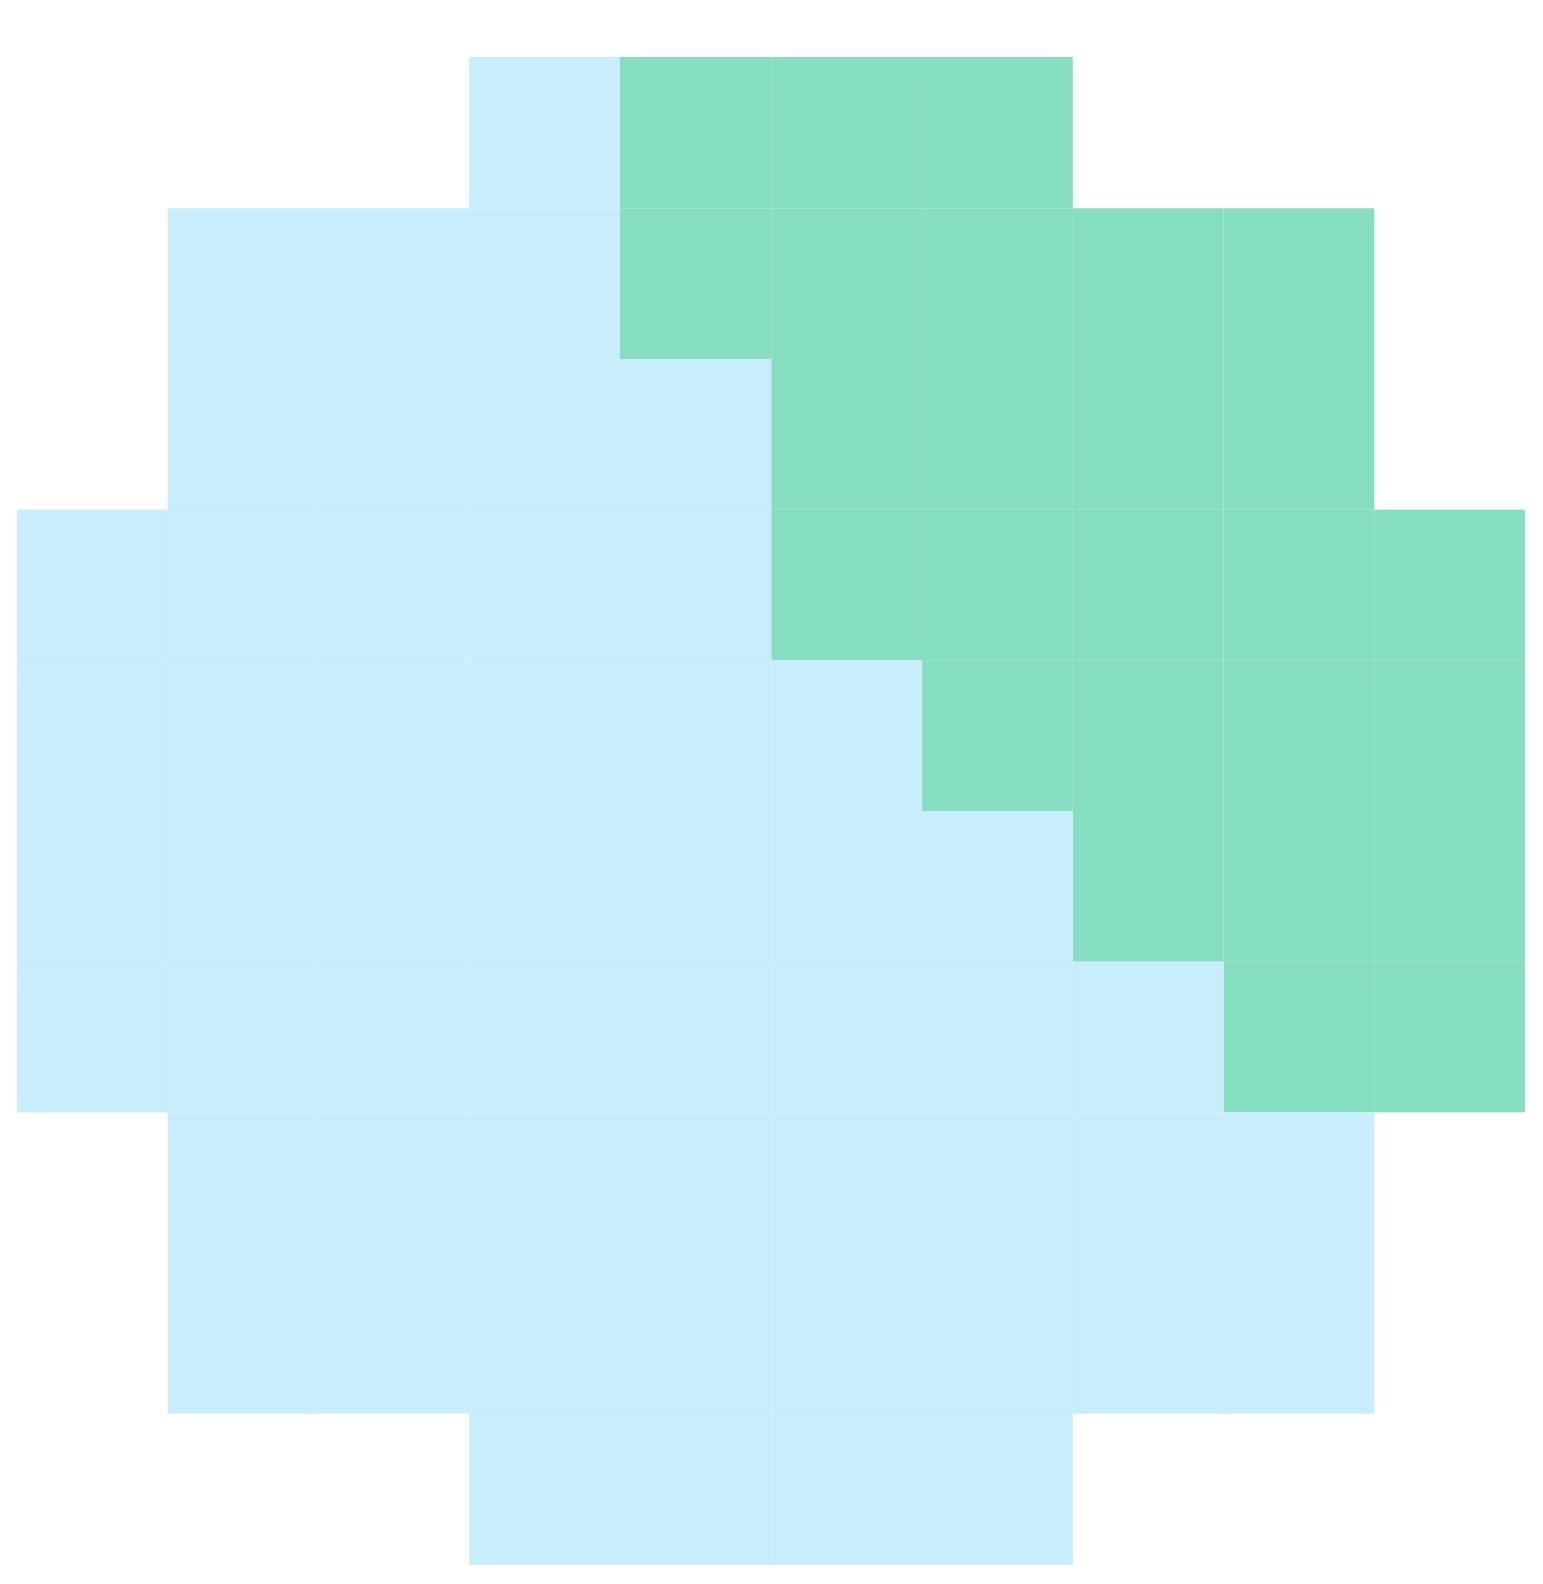
\includegraphics[scale=0.57]{media/2-shabaka/1-vor/dem1.png}
\label{fig:vor1}}
\subfigure[]{%
		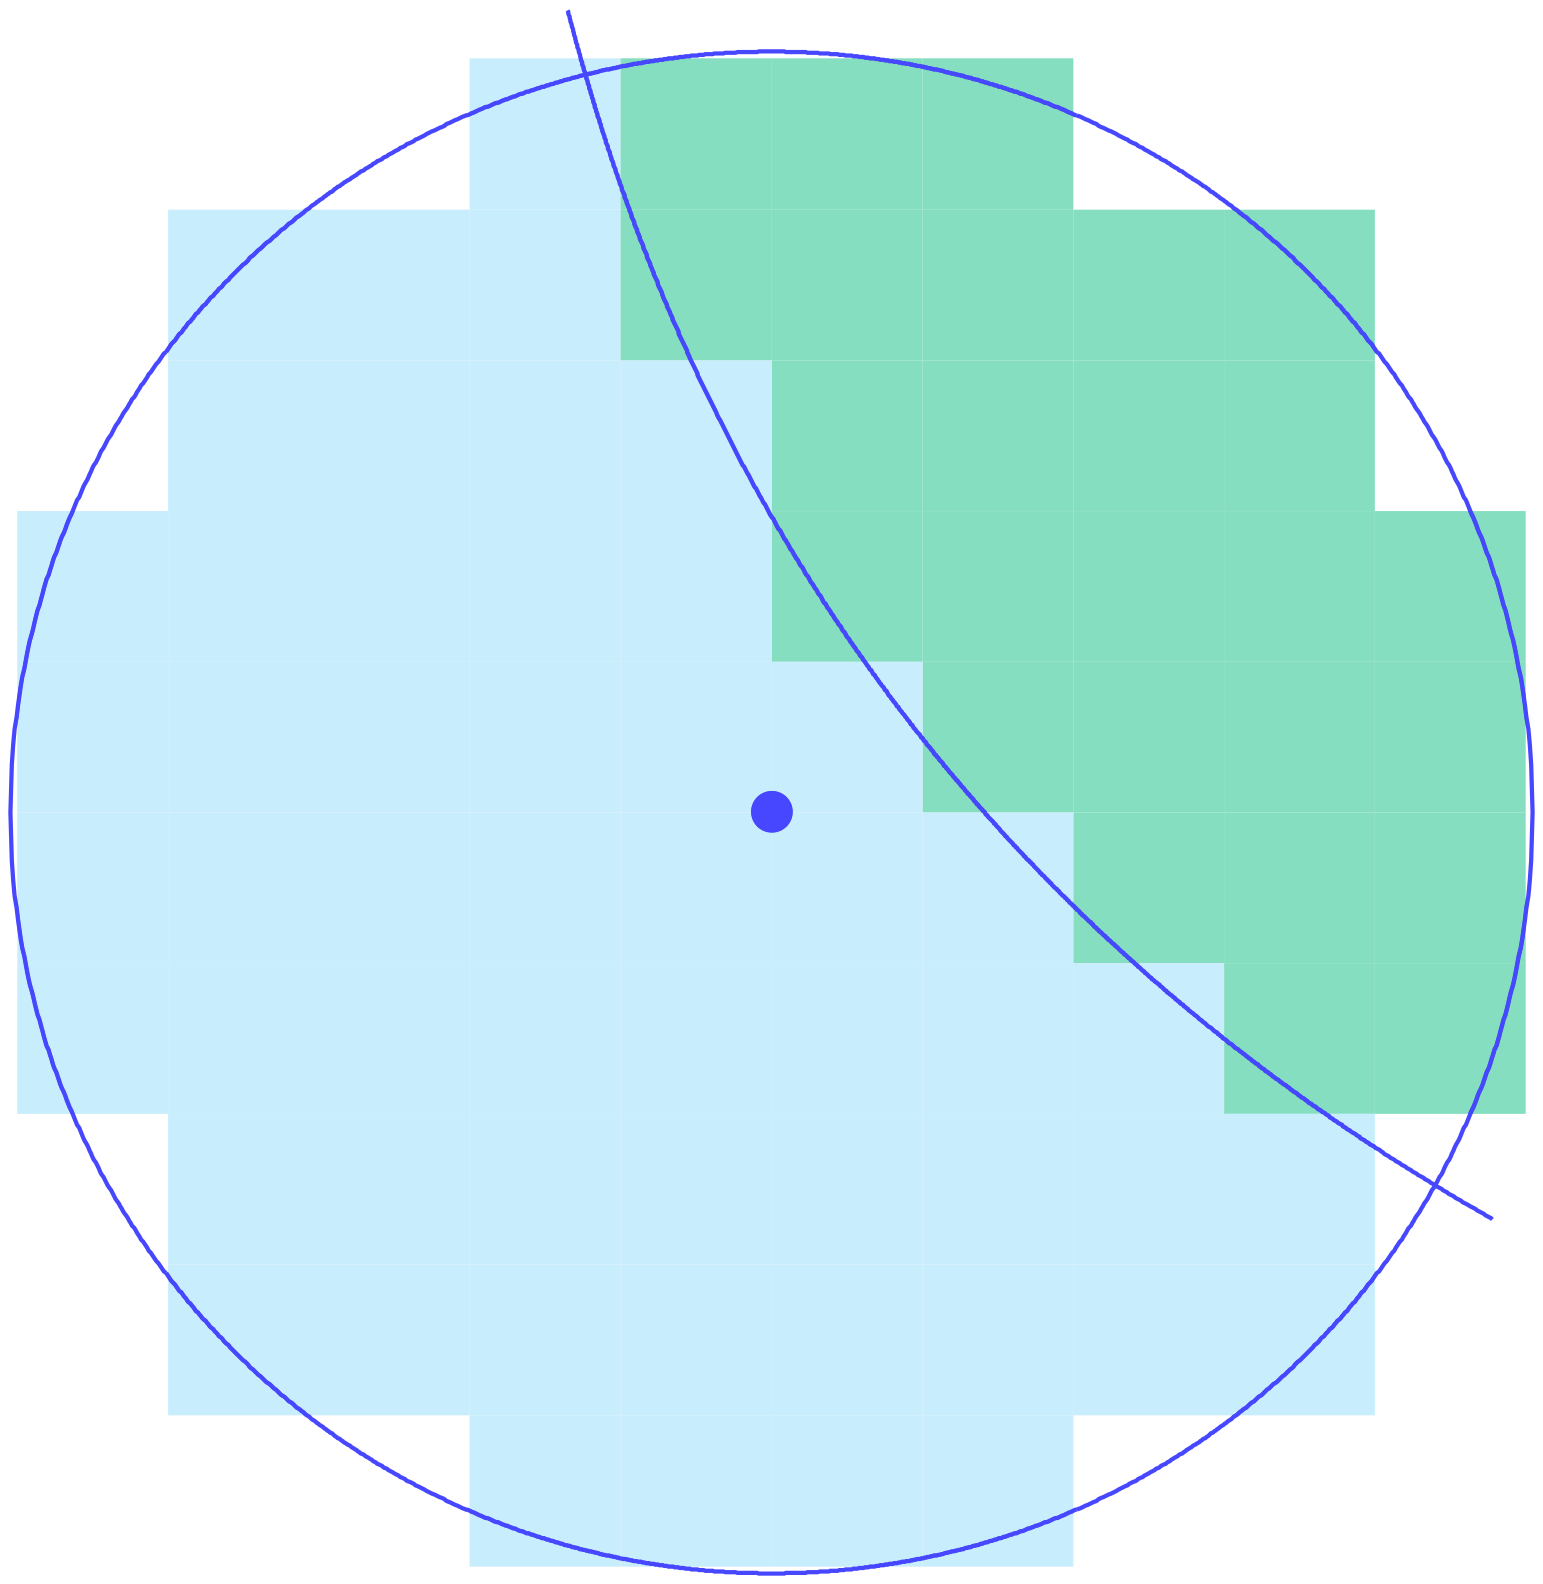
\includegraphics[scale=0.57]{media/2-shabaka/1-vor/dem2.png}
\label{fig:vor2}}
\subfigure[]{%
		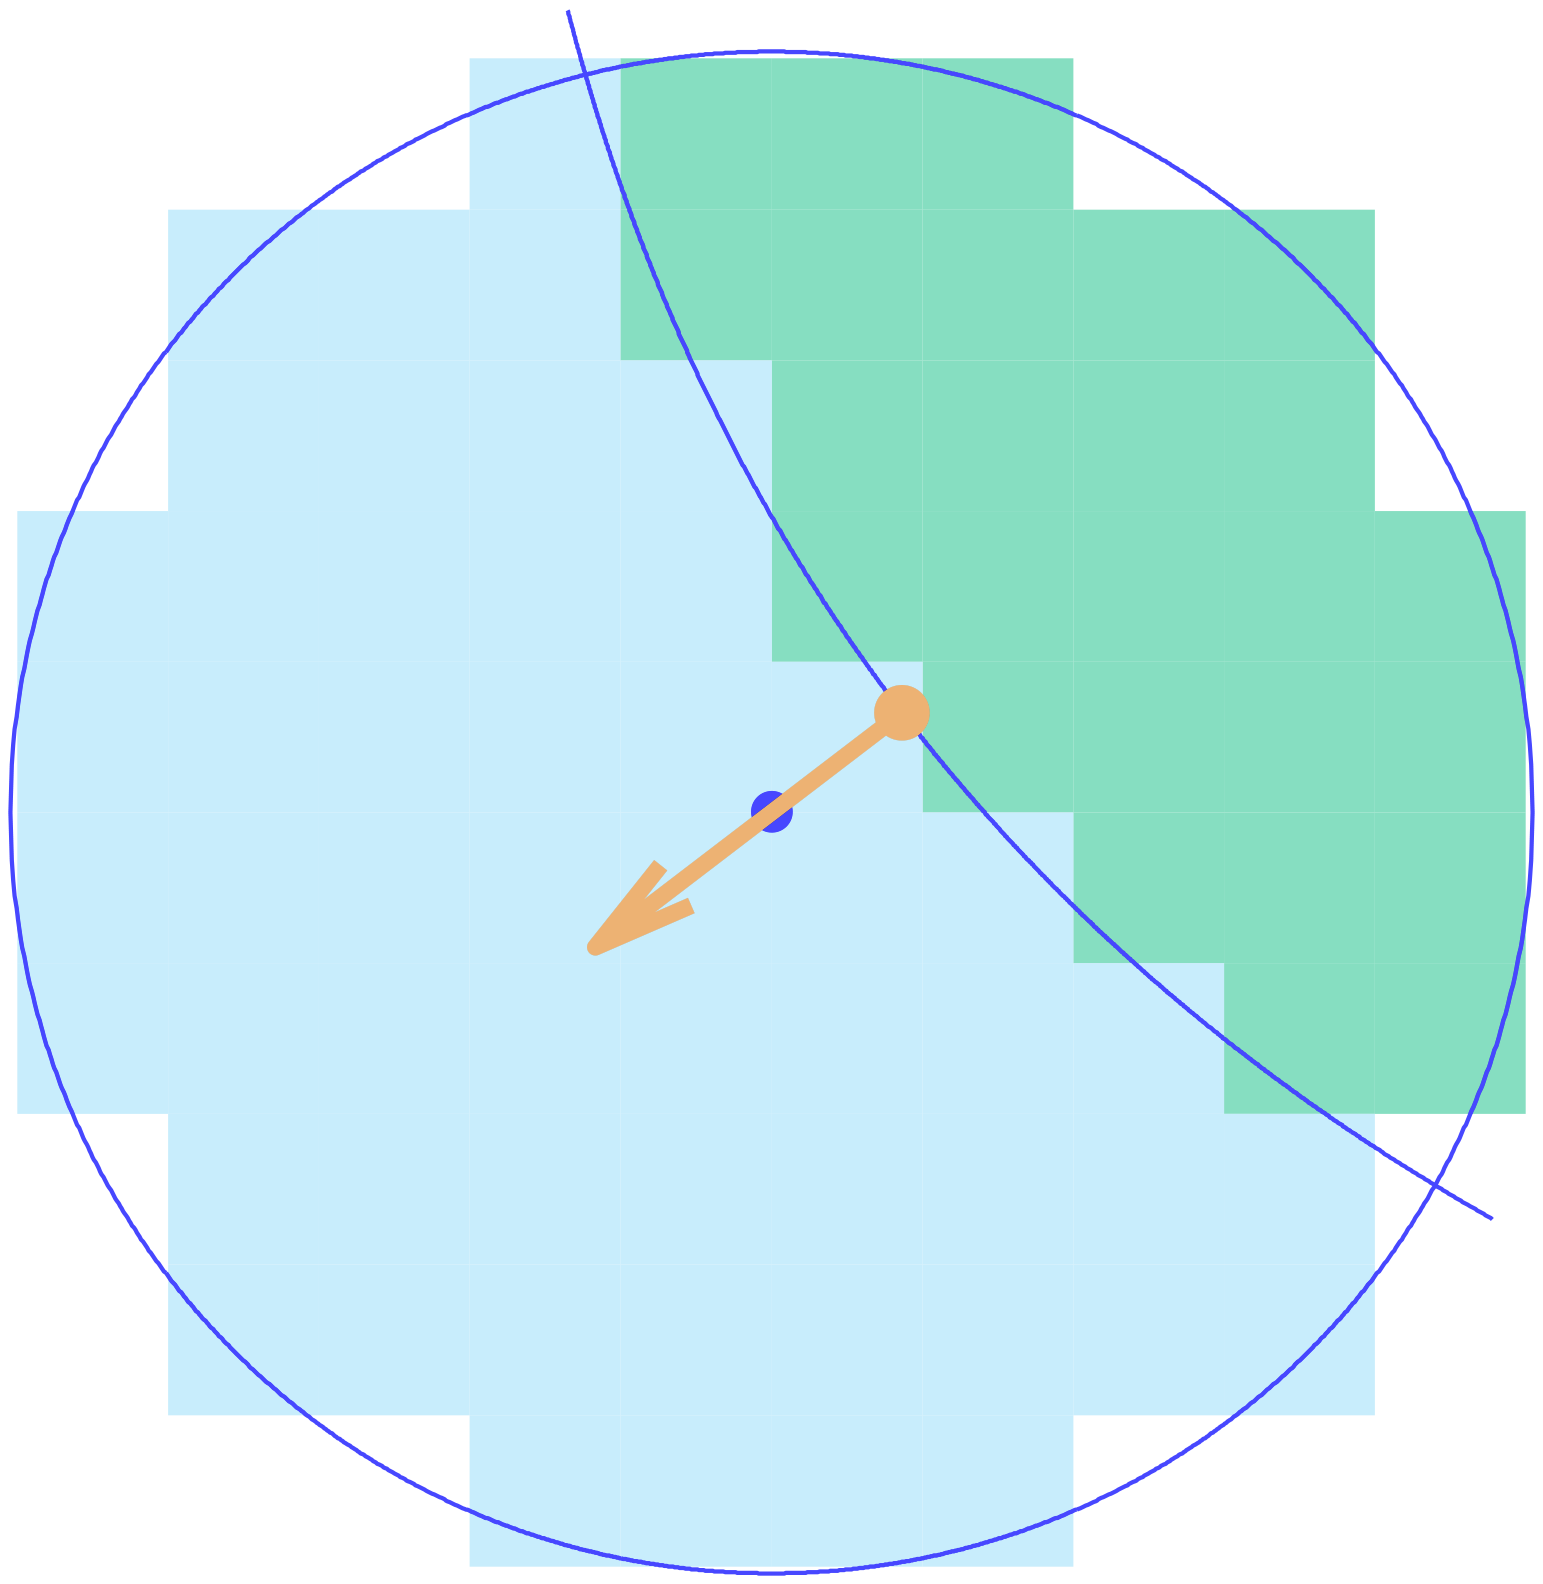
\includegraphics[scale=0.57]{media/2-shabaka/1-vor/dem3.png}
\label{fig:vor3}}
\subfigure[]{%
		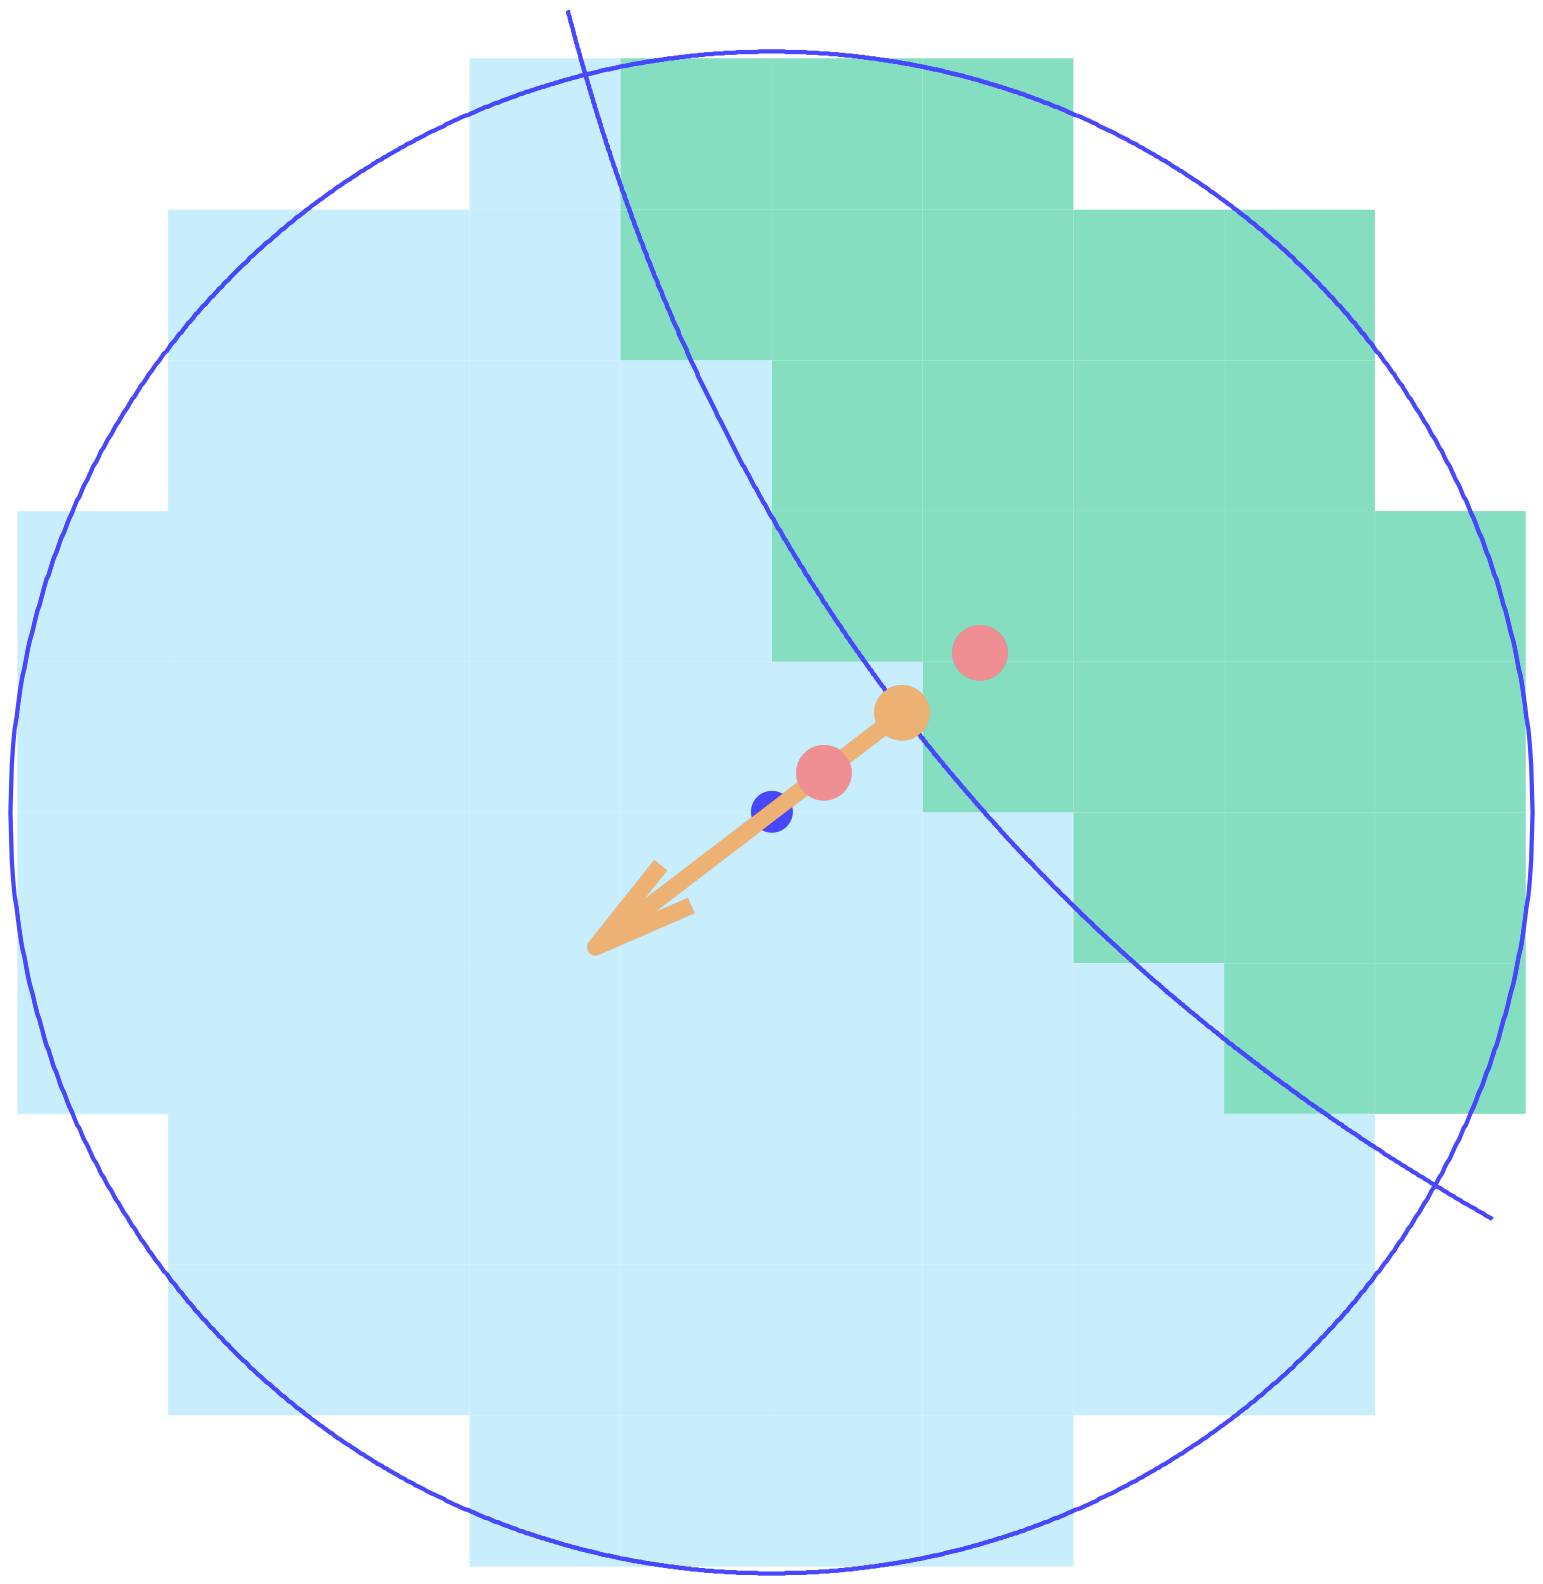
\includegraphics[scale=0.57]{media/2-shabaka/1-vor/dem4.png}
\label{fig:vor4}}
%
\caption{(a) Sampling window of the segmented image, (b) boundary approximation, (c) point/normal placement, and d) Voronoi site placement. Green voxels indicate solid material and blue voxels are void.  Note the presence of isolated mis-colored voxels.  The sampling window center is shown in dark blue, point/normal boundary pair in orange, and Voronoi sites in red.}
\label{fig:vor}
\end{figure}

\subsubsection{Window Selection}

We denote the set of all voxels in a segmented image as $\mathcal{I}$. The segmented image  $\mathcal{I}$ is sampled with overlapping windows, each of which is a voxelized sphere with voxel radius $R_{\mathcal{W}}$ (an integer). The translation in each Cartesian direction between adjacent windows is $d_{\mathcal{W}}$, which is also an integer voxel count. The set of voxels in a particular window is denoted $\mathcal{W}$, and the number of voxels in that window is $n_{\mathcal{W}}$. We further define the subset of voxels in $\mathcal{W}$ that are designated as solid material to be $\mathcal{M}$, with $n_{\mc{M}} = | \mc{M} |$. \\ \\
%
A window $\mathcal{W}$ is marked for further processing if it satisfies a threshold requirement, as follows.  Letting $k_{\mathcal{M}} = n_{\mathcal{M}}/n_{\mathcal{W}}$, we define a threshold value $\overline{k}_{\mathcal{M}}$ such that the window is retained only if $k_{\mathcal{M}} \in (\overline{k}_{\mathcal{M}}, 1 - \overline{k}_{\mc{M}})$.  Thus, further calculations are performed only if sufficiently many voxels of both solid material and of void are present in the window to support approximation of a material boundary. Refer to~\tabref{window} for a summary of these variables definitions.

\begin{table}[htbp!]
 \centering
   \begin{tabular}{|c||c|}
   \hline
   {\textbf{Variable}} & \textbf{Description} \\ \hline \hline
   $\mathcal{I}$ & set of all voxels in a segmented image \\ \hline
   $\mathcal{W}$ & set of all voxels in a specified window \\ \hline
   $\mc{M}$ & subset of $\mc{W}$ occupied by the material of interest\\ \hline
   {$k_{\mathcal{M}}$} & ratio of voxels in $\mathcal{M}$ to voxels in $\mathcal{W}$\\ \hline
   {$\overline{k}_{\mathcal{M}}$ \rule{0mm}{4mm}} & threshold value for $k_{\mathcal{M}}$ \\ \hline 
   $R_{\mathcal{W}}$ & window radius (in voxels) \\ \hline
   $d_{\mathcal{W}}$ & sampling distance between adjacent windows (in voxels) \\ \hline  
\end{tabular}
\caption{List of variables relevant to the windowing scheme.}
\label{tab:window}
\end{table}

\subsubsection{Local Boundary Approximation}

Given a window $\mathcal{W}$ that is marked as intersecting the body boundary, we seek to derive a local boundary-surface patch $\mc{S}$ that optimally represents the boundary separating $\mc{M}$ and $\mc{W} \setminus \mc{M}$.  The overall plan is as follows: we define geometrically smooth (i.e., not voxelated), disjoint, simply connected regions that approximate $\mc{W}$ and $\mc{M}$, whose common boundary serves to define the surface patch $\mc{S}$.  The regions and the surface $\mc{S}$ are chosen to have simple, parameterizable shapes; optimally fitting them to $\mc{W}$ and $\mc{M}$ therefore reduces to a small algebraic minimization problem.  We require that $\mc{S}$ be non-self-intersecting, and that it divides the smooth approximation to $\mc{W}$ into exactly two subregions. 
Proceeding in this direction, let $\mc{D}$ be a sphere whose center and radius $R$ are chosen such that the centroid and volume of $D$ match those of $\mc{W}$.  Next, we define $\Omega_p$ as the spatial region occupied by $\mc{M}$, and $\Omega$ as the subset of $\mc{D}$ that lies on the material side of $\mc{S}$.  We assume that $\mc{S}$ intersects $\partial \mc{D}$ in a simple closed loop, so that $\Omega$ is a simply-connected subset of $\mc{D}$ that resembles a lens. The situation is illustrated in \figref{figure3} in 2D.
\begin{figure}[b!]
	\centering
	\subfigure[Window $\mathcal{W}$]{%
		
\includegraphics[scale=0.72]{media/om/dem2.pdf}
		\label{fig:subfigure2}}
	\subfigure[Approximating circle $\mathcal{D}$]{%
		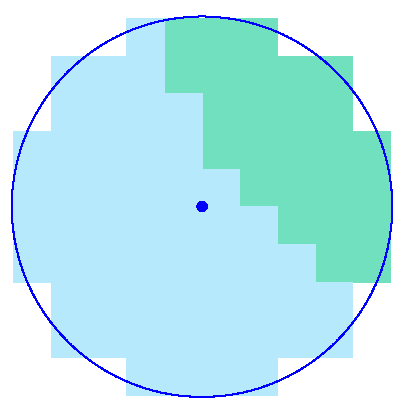
\includegraphics[scale=0.72]{media/om/dem3.pdf}
		\label{fig:subfigure3}}
	
	\subfigure[Approximating surface $\mathcal{S}$]{%
		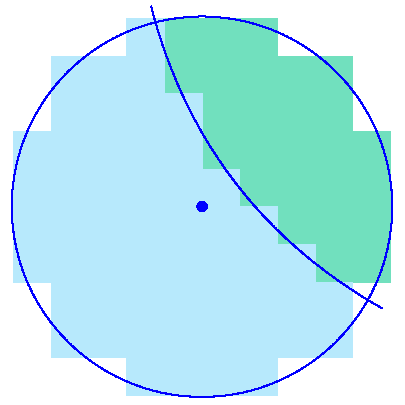
\includegraphics[scale=0.72]{media/om/dem4.pdf}
		\label{fig:subfigure4}}
	\subfigure[Voxelated region $\Omega_p$]{%
		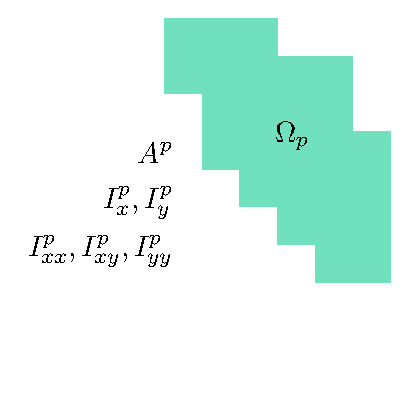
\includegraphics[scale=0.72]{media/om/omp.pdf}
		\label{fig:subfigure5}}
	\subfigure[Approximating lens $\Omega$]{%
		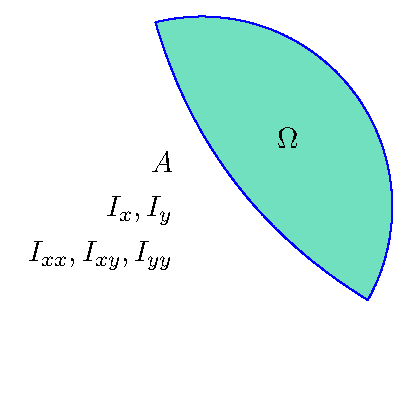
\includegraphics[scale=0.72]{media/om/om.pdf}
		\label{fig:subfigure6}}
	
	\caption{Boundary approximation demonstrated in 2D.}
	\label{fig:figure3}
\end{figure}\noindent
It remains to provide a concrete parameterization of $\mc{S}$, and a specific objective function through which $\Omega$ is optimally fitted to $\Omega_p$.  To these ends, in this initial exposition we take $\mc{S}$ to be a plane, as shown in \figref{quad}. We define an objective function via the zeroth, first, and second polynomial moments of $\Omega_p$ and $\Omega$: 
\begin{alignat}{5}
&{} &&V^p = \int_{\Omega_p}dv, &&{} \\
I_{x\phantom{z}}^p &= \int_{\Omega_p}xdv, &&I_{y\phantom{z}}^p = \int_{\Omega_p}ydv, &&I_{z\phantom{z}}^p = \int_{\Omega_p}zdv, \\
I^p_{xy} &= \int_{\Omega_p}xydv, &&I^p_{xz} = \int_{\Omega_p}xzdv, &&I^p_{yz} = \int_{\Omega_p}yzdv, \\
I^p_{xx} &= \int_{\Omega_p}(y^2 + z^2)dv, \text{\ \ \ \ \ \ }&&I^p_{yy} = \int_{\Omega_p}(x^2 + z^2)dv, \text{\ \ \ \ \ \ }&&I^p_{zz} = \int_{\Omega_p}(x^2 + y^2)dv.
\end{alignat}
Analogous quantities $V$, $I_x$, etc. are defined for $\Omega$.  Placing the coordinate origin at the common centroid of $\mc{W}$ and $\mc{D}$, the planar surface $\mc{S}$ is defined by the signed value $x' = d$, where the primed coordinates are oriented such that the $x'$ axis is normal to $\mc{S}$.  See \figref{quad}.
\begin{figure}[t!]
	\centering
		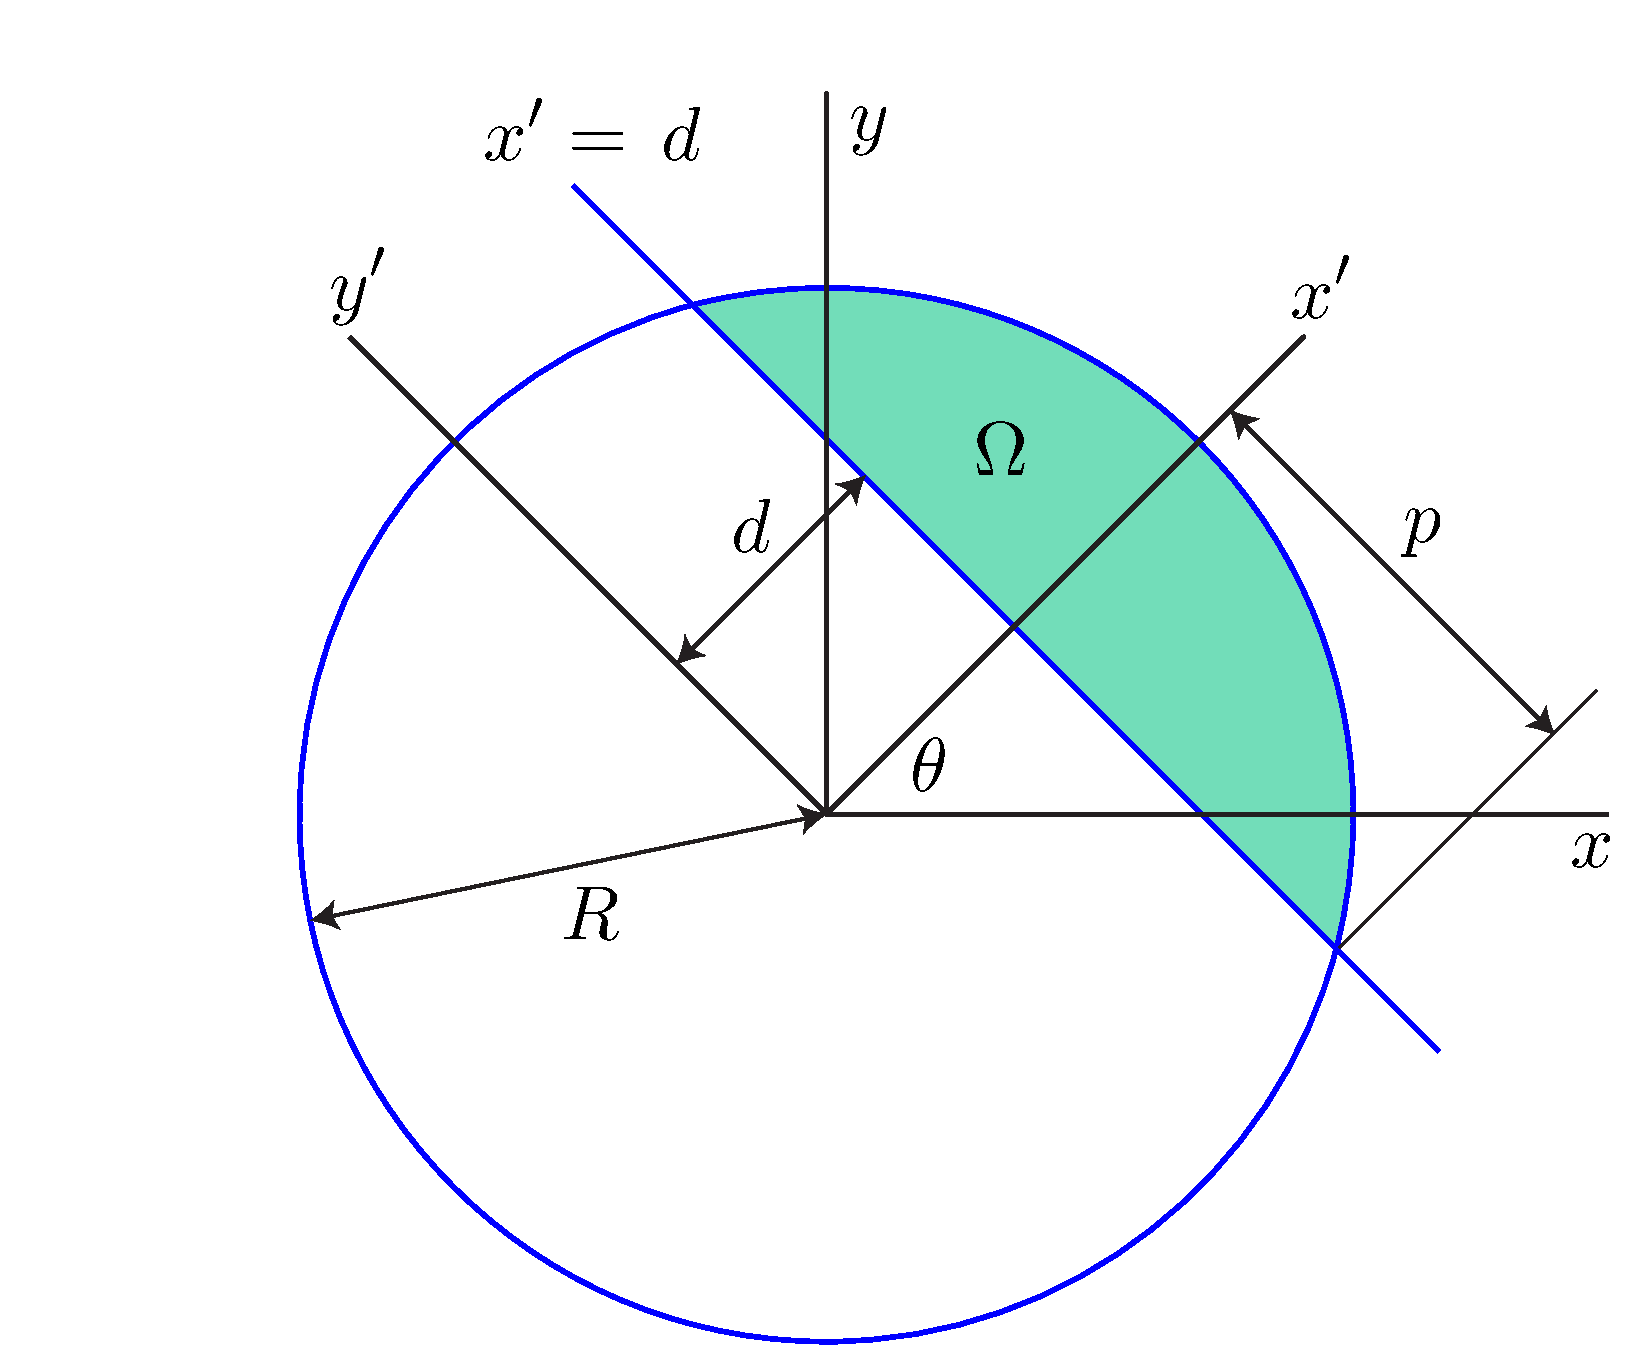
\includegraphics[scale=0.3]{media/om/window.pdf}
	\caption{Plane boundary approximation demonstrated in 2D.}
	\label{fig:quad}
\end{figure}\noindent

Turning now to the formulation of the error function, we define the following quantities:
\begin{alignat}{3}
f^p &= V^p, \text{\ \ \ \ \ }&&f(d,\psi,\theta) = V, \\
\bm{g}^p &= \left[\begin{array} {ccc} {I_x^p} \\ {I_y^p} \\ {I_z^p} \end{array} \right], \text{\ \ \ \ \ }&&\bm{g}(d,\psi,\theta) = \left[\begin{array} {ccc} {I_x} \\ {I_y} \\ {I_z} \end{array} \right], \\
\bm{h}^p &= \left[\begin{array} {ccc} {I_{xx}^p} & {-I_{xy}^p} & {-I_{xz}^p}\\ {-I_{xy}^p} & {I_{yy}^p} & {-I_{yz}^p} \\ -{I_{xz}^p} & {-I_{yz}^p} & {I_{zz}^p} \end{array} \right],\text{\ \ \ \ \ \ \ }&&\bm{h}(d,\psi,\theta) = \left[\begin{array} {ccc} {I_{xx}} & {-I_{xy}} & {-I_{xz}}\\ {-I_{xy}} & {I_{yy}} & {-I_{yz}} \\ -{I_{xz}} & {-I_{yz}} & {I_{zz}} \end{array} \right].
\end{alignat}
Relative errors in the zeroth, first, and second polynomial moments of the window's solid subdomain are then defined as:

\begin{align}
e_0(d,\psi,\theta) &=  \sqrt{\frac{(f - f^p)^2}{(f^p)^2}}, \\
e_1(d,\psi,\theta) &=  \sqrt{\frac{(g_i - g_i^p)(g_i - g_i^p)}{g_j^{p}g_j^{p}}}, \\
e_2(d,\psi,\theta) &=  \sqrt{\frac{(h_{ij} - h_{ij}^p)(h_{ij} - h_{ij}^p)}{h_{kl}^{p}h_{kl}^{p}}}.
\end{align}
\textcolor{purple}{where index notation is employed for the vector and tensor quantities $\bm{g}^p$, $\bm{g}$, $\bm{h}^p$, and $\bm{h}$, and the summation convention on repeated indices is in force}. Finally, we define a single scalar error function as:
\begin{align}
\label{obj func}
\mathcal{F}(d,\psi,\theta) = \beta_0e_0 + \beta_1e_1 + \beta_2e_2,
\end{align}
where $\beta_i$ are adjustable weights in the range $(0,1)$ and $\sum \limits_i\beta_i = 1$.  The error $\mc{F}$ is an explicit function of the parameters $d$, $\psi$, and $\theta$, where $\psi$ and $\theta$ are the orientation angles of the plane normal relative to the voxel axes $(x, y, z)$, and $d$ is the plane's offset from the centroid of the window.

We seek the solution to the following unconstrained minimization problem: $\displaystyle \min_{d, \psi, \theta} \mathcal{F}(d,\psi,\theta)$, which can be solved by a variety of well-established techniques once the moments of $\Omega$ and $\Omega_p$ are defined. The moments of $\Omega_p$ are computed based on a straightforward use of voxel dimensions and the parallel axis theorem. The moments of $\Omega$, on the other hand, are first computed as a function of $d$ in the primed coordinate system, and then transformed to the $(x, y, z)$ frame based on $\psi$ and $\theta$. The relevant geometric quantities in the primed system are computed as follows:
\begin{align}
\color{purple}{p^2} &\color{purple}{= R^2 - d^2}\color{black}{,} \\
V^* &= 2\pi\left[-\frac{1}{2}dp^2 + \frac{1}{3}R^3 - \frac{1}{3}(R^2 - p^2)^{3/2} \right], \\
I^*_{x'x'} &= \frac{\pi}{30}\left[-15dp^4 + \sqrt{R^2-p^2}\left(12p^4 - 4p^2R^2 - 8R^4\right) + 8R^5 \right], \\
I^*_{y'y'} &= \frac{\pi}{480}\left[-160d^3p^2 + 128R^5 - \sqrt{R^2-p^2}\left(128R^4 - 96p^2R^2 - 32p^4\right) - 120dp^4 \right],
\end{align}
\begin{align} 
V &=  \begin{cases}
      V^*, & \text{if}\ d \geq 0 \\
      V^* + \frac{4\pi}{3}\left(R^2-p^2\right)^{3/2}, & \text{otherwise}
    \end{cases}\\
I_{x'} &= \frac{\pi}{4}\left[2p^2(R^2-d^2) - p^4 \right],\\
I_{y'} &= I_{z'} = 0, \\
I_{x'y'} &= I_{x'z'} = I_{y'z'} = 0, \\
I_{x'x'} &=  \begin{cases}
      I^*_{x'x'}, & \text{if}\ d \geq 0 \\
       I^*_{x'x'} + \frac{4\pi}{15}(R^2-p^2)^{3/2}(3p^2+2R^2), & \text{otherwise}
    \end{cases} \\
I_{y'y'} &=  \begin{cases}
     I^*_{y'y'}, & \text{if}\ d \geq 0 \\
     I^*_{y'y'} + \frac{2\pi}{15}(R^2-p^2)^{3/2}(p^2+4R^2), & \text{otherwise}
    \end{cases} \\
I_{z'z'} &= I_{y'y'}.
\end{align}
As expected, some moments exhibit symmetries about the $y'$ and $z'$ axes. \\ \\

The moments are transformed back to the global voxel-grid frame so that they can be compared to those of $\Omega_p$. This transformation is different for the zeroth, first, and second polynomial moments due to the different tensor rank for each of these quantities. The first and second polynomial moments are transformed in the following manner (no transformation is required for the zeroth moment):
\begin{gather}
\bm{R} = \left[\begin{array} {ccc} {\cos\psi\cos\theta} & {-\sin\psi} & {\cos\psi\sin\theta}\\ {\sin\psi\cos\theta} & {\cos\psi} & {\sin\psi\sin\theta}, \\
{-\sin\theta} & {0} & {\cos\theta}\end{array} \right], \\
\left[\begin{array} {ccc} {I_x} \\ {I_y} \\ {I_z} \end{array} \right] = \bm{R} \left[\begin{array} {ccc} {I_{x'}} \\ {I_{y'}} \\ {I_{z'}} \end{array} \right], \\
\bm{I}' = \left[\begin{array} {ccc} {I_{x'x'}} & {-I_{x'y'}} & {-I_{x'z'}}\\ {-I_{x'y'}} & {I_{y'y'}} & {-I_{y'z'}} \\ -{I_{x'z'}} & {-I_{y'z'}} & {I_{z'z'}} \end{array} \right], \\
\bm{I} = \left[\begin{array} {ccc} {I_{xx}} & {-I_{xy}} & {-I_{xz}}\\ {-I_{xy}} & {I_{yy}} & {-I_{yz}} \\ -{I_{xz}} & {-I_{yz}} & {I_{zz}} \end{array} \right] = \bm{R}\bm{I}'\mathbf{R}^T.
\end{gather}
\noindent With all relevant quantities in place, the \textit{subplex search method}~\cite{rowan} is used to minimize the error function (\ref{obj func}) using an implementation in the package \textit{NLopt} \cite{nlo}. The method is a derivative-free method that is well-suited for optimizing objective functions that are noisy or discontinuous. It was selected as the optimization approach due to the existence of square roots in the objective function, and the fact that robustness to a wide range of inputs was the highest priority in developing the algorithm. \\ \\
%
Convergence is assumed to be achieved when $\left| \mathcal{F}_{k+1} - \mathcal{F}_{k}\right| < \varepsilon$ on successive iterations, where $k$ is the iteration number and  $\varepsilon$ is the convergence tolerance. For the specific examples and algorithm parameters discussed later in this section, convergence is achieved for each boundary approximation after typically hundreds of iterations. This large value may be due to the admittedly tight tolerance for $\varepsilon$ of $10^{-14}$; to nonlinearities or saddle points in the error function; or to inefficiencies in the nonlinear optimization tool used. However, the algorithm generates high-quality results, and the process for all windows usually completes in less than one minute of wall clock time on a personal computer, even for complex geometries. Thus, convergence rate was not further explored as a means of improving the algorithm. \\ \\
%
Finally, we require that once convergence has been satisfied, the criterion $\mathcal{F} < \overline{\mathcal{F}}$ must also be met for the point and normal to be retained. In this way, when $\Omega$ unsatisfactorily approximates $\Omega_p$, the associated point and normal are discarded. This typically occurs in regions of high curvature, where a plane does not approximate the boundary well. The point cloud is dense enough that simply discarding these outlier points does not cause any discernible amount of undersampling of the surface. \\ \\
%
The solution to the minimization problem yields the values $d$, $\psi$, and $\theta$ that determine the optimal surface $\mathcal{S}$, from which the boundary point and normal are defined. \tabref{surface} can be consulted for a complete summary of variables discussed regarding local boundary approximation. \\

\begin{table}[t!]
 \centering
   \begin{tabular}{|c||c|}
   \hline
   {\textbf{Variable}} & {\textbf{Description}} \\ \hline \hline
   $\mathcal{D}$ & approximating sphere to $\mathcal{W}$ \\ \hline
   $\mathcal{S}$ & approximating surface to boundary of interest \\ \hline      
   $R$ & radius of $\mathcal{D}$ \\ \hline   
   $\Omega_p$ & physical space covered by voxels belonging to $\mathcal{W}$ \\ \hline
   $\Omega$ & physical space covered by approximating lens of $\Omega_p$ \\ \hline      
   $(x,y,z)$ & axes aligned with image directions, whose origin is at the center of $\mathcal{W}$\\ \hline
   {$(x',y',z')$} & axes $(x,y,z)$ transformed such that $x'$ passes through centroid of $\Omega$ \\ \hline
%   {} & where $x'$ passes through the centroid of $\Omega$ \\ \hline   
   $d$ & perpendicular distance from center of $\mathcal{D}$ to plane $\mathcal{S}$  \\ \hline
   $\psi$ & yaw angle of rotation between $(x,y,z)$ and $(x',y',z')$ axes \\ \hline   
   $\theta$ & pitch angle of rotation between $(x,y,z)$ and $(x',y',z')$ axes \\ \hline
   $V^p$ & (zeroth moment of) volume of $\Omega_p$ \\ \hline
   $I_{x}^p, I_y^p$ & first moments of volume of $\Omega_p$ \\ \hline     
   $I_{xy}^p, I_{xz}^p, I_{yz}^p$ & product moments of volume of $\Omega_p$ \\ \hline      
   $I_{xx}^p, I_{xy}^p, I_{yy}^p$ & second moments of volume of $\Omega_p$ \\ \hline
   $V$ & (zeroth moment of) volume of $\Omega$ \\ \hline
   $I_{x}, I_y$ & first moments of volume of $\Omega$ \\ \hline
   $I_{xy}, I_{xz}, I_{yz}$ & product moments of volume of $\Omega$ \\ \hline   
   $I_{xx}, I_{xy}, I_{yy}$ & second moments of volume of $\Omega$ \\ \hline
   $e_0$ & relative error in zeroth polynomial moment \\ \hline
   $e_1$ & relative error in first polynomial moments \\ \hline
   $e_2$ & relative error in second polynomial moments \\ \hline   
   $\beta_0$ & weighting coefficient for error in zeroth polynomial moment \\ \hline
   $\beta_1$ & weighting coefficient for error in first polynomial moments \\ \hline
   $\beta_2$ & weighting coefficient for error in second polynomial moments \\ \hline 
   $\varepsilon$ & convergence tolerance for minimization of function $\mathcal{F}$ \\ \hline
   $\overline{\mathcal{F}}$ \rule{0mm}{4mm} & largest acceptable value of function $\mathcal{F}$ \\ \hline        
\end{tabular}
\caption{List of variables in local boundary approximation.}
\label{tab:surface}
\end{table}

\subsubsection{Boundary Point and Normal Placement}

Once the parameters $d$, $\psi$, and $\theta$ are selected for a particular window $\mathcal{W}$, a point location and outward normal must be determined. The outward-pointing normal is the negative of the first column of the transformation matrix $\bm{R}$: $\bm{n} = -(\cos\psi\cos\theta,\text{\ }\sin\psi\cos\theta,\text{\ }-\sin\theta)$. With the origin at the center of sphere $\mathcal{D}$, the location of the surface point is then simply $\mathbf{x}_p = -d\bm{n}$.

%%%%%%%%%%%%%%%%%%%%%%%%%%%%%%%%%%%%%%%%%%%%%%%
%%%%%%%%%%%%%%%%%%%%%%%%%%%%%%%%%%%%%%%%%%%%%%%
\subsection{Surface Reconstruction \textcolor{purple}{Algorithm}}
\label{Surface Reconstruction}

Surface reconstruction is the process of generating closed, manifold, polygonized surfaces from point clouds. Approaches found in the existing literature typically assume a dense, noisy population of points that are usually generated by structured light or laser-based scanners. Though the proposed algorithm departs from these assumptions to a degree, a brief review of surface reconstruction techniques is still worthwhile. \\ \\
%
Among the most well-known surface reconstruction algorithms are the \textit{Power Crust} and \textit{Poisson surface reconstruction} techniques. Amenta \textit{et al.}~\cite{amenta_2001} presented the \textit{Power Crust} algorithm for reconstructing watertight surfaces from unoriented point clouds. The algorithm first constructs the \textit{medial axis transform} from the point cloud, which consists of the set of maximal balls completely contained in the interior of the surface. The algorithm then applies an inverse transform to approximate the medial axis and produce a piecewise linear surface. The algorithm does not perform well when the point set is not sufficiently dense. Kazhdan \textit{et al.} presented \textit{Poisson surface reconstruction}~\cite{kazhdan_2008} and subsequently \textit{screened Poisson surface reconstruction}~\cite{kazhdan_2013} for oriented point clouds. They compute an indicator function defined as 1 for points inside the surface and 0 for points outside, whose gradient approximates the vector field defined by the oriented point cloud. This amounts to solving a Poisson problem for an implicit indicator function, followed by application of marching cubes to polygonize the surface. The \textit{screened} approach provides a soft constraint that encourages the reconstructed isosurface to pass through the input points. In practice, the screened approach is more robust than the original Poisson approach in generating manifold surfaces from complex point clouds. The technique produces smooth surfaces that exhibit resiliency to noise, outliers, and undersampling that makes it perhaps the best available method in many cases. \\ \\
%
Many other surface reconstruction approaches exist, including those making use of moving least squares, Delaunay and Voronoi constructions, and variational approaches~\cite{berger}. A novel Voronoi-based approach is presented here as an alternative to these approaches, which is tuned to address the type of noise and point density expected from the point-cloud-generation step described previously. \\ \\
%
The proposed surface reconstruction technique relies on constructing a \textit{Voronoi partition}, which for our purposes is a nearest neighbor partitioning of $\mathbb{R}^3$ based on a set of input \textit{Voronoi sites}. The desired output from a Voronoi partition is a mesh -- namely, a set of points, edges, facets, and cells (and their connectivities) that discretize space. We first define the half-space $D(\bm{p},\bm{q})$, comprising all points $\bm{x}$ as close, or closer, to site $\bm{p}$ than to site $\bm{q}$:
\begin{equation}
D(\bm{p},\bm{q}) = \{\bm{x} \mid d(\bm{p},\bm{x}) \leq d(\bm{q},\bm{x})\},
\end{equation}
where a distance function $d$ must be defined. Although there exist more exotic distance functions leading to modified Voronoi partitions, the distance function for standard Voronoi diagrams is simply the Euclidean distance. Defining $\mathcal{P}$ to be the set of Voronoi sites, the \textit{Voronoi cell} $V(\bm{p})$ associated with site $\bm{p}$ is the intersection of all half-spaces involving site $\bm{p}$ and all other sites $\bm{q}$ belonging to $\mathcal{P}$:
\begin{equation}
V(\bm{p}) = \bigcap \limits_{\bm{q} \in \mathcal{P}, \bm{q} \neq \bm{p}} D(\bm{p},\bm{q}).
\end{equation}
A number of important properties exist for Voronoi partitions and their dual \textit{Delaunay tessellations}. For the present purposes, the most important property is that the surface extracted from a set of Voronoi cells connected by shared facets is watertight and manifold. Several important considerations must be accounted for in constructing a Voronoi partition, including degenerate and near-degenerate cases, the data schema and order of construction of the connected polytopes, and the performance of the algorithm. Refer to Aurenhammer~\cite{aurenhammer_1991} for a detailed survey of the mathematical and algorithmic approaches to Voronoi diagrams. \\ \\
%
The proposed technique involves the following steps, to be described in turn:
\vspace{2mm}
\begin{itemize}[noitemsep]
\item Generate the Voronoi site set from the oriented point cloud and perform Voronoi partition of image.
\item Extract the b-rep as the set of facets that share Voronoi sites with different material types and perform cleanup on that surface.
\item Decimate and smooth the surface to a more tractable mesh resolution.
\end{itemize}

\subsubsection{Voronoi Site Generation and Voronoi Partitioning}

Given the location of a boundary point $\bm{x}_p$ and orientation of its corresponding normal $\bm{n}$, two Voronoi sites are placed on either side of the point along the normal, as shown in~\figref{vor4} and~\figref{d2dvor3}. They are separated from the point by a distance $b$; hence, their locations are $\bm{x}_p \pm b \bm{n}$. The two Voronoi sites are assigned material types. For the two-material case considered here, the site corresponding to the position $\bm{x}_p - b\bm{n}$ is inside $\Omega$, and thus is assigned to the material of interest. The site corresponding to the position $\bm{x}_p + b\bm{n}$ is designated as void material. Voronoi partitioning is performed using an implementation from \textit{Qhull}~\cite{barber_1996} that is robust even for near-degenerate Voronoi site locations. The sequence of point cloud generation, Voronoi site placement, and Voronoi partitioning is illustrated in~\figref{d2dvor}.

\begin{figure}[htbp!]
\centering
\subfigure[]{%
		
\includegraphics[scale=0.47]{media/vv/a111.png}
\label{fig:d2dvor1}}
\subfigure[]{%
		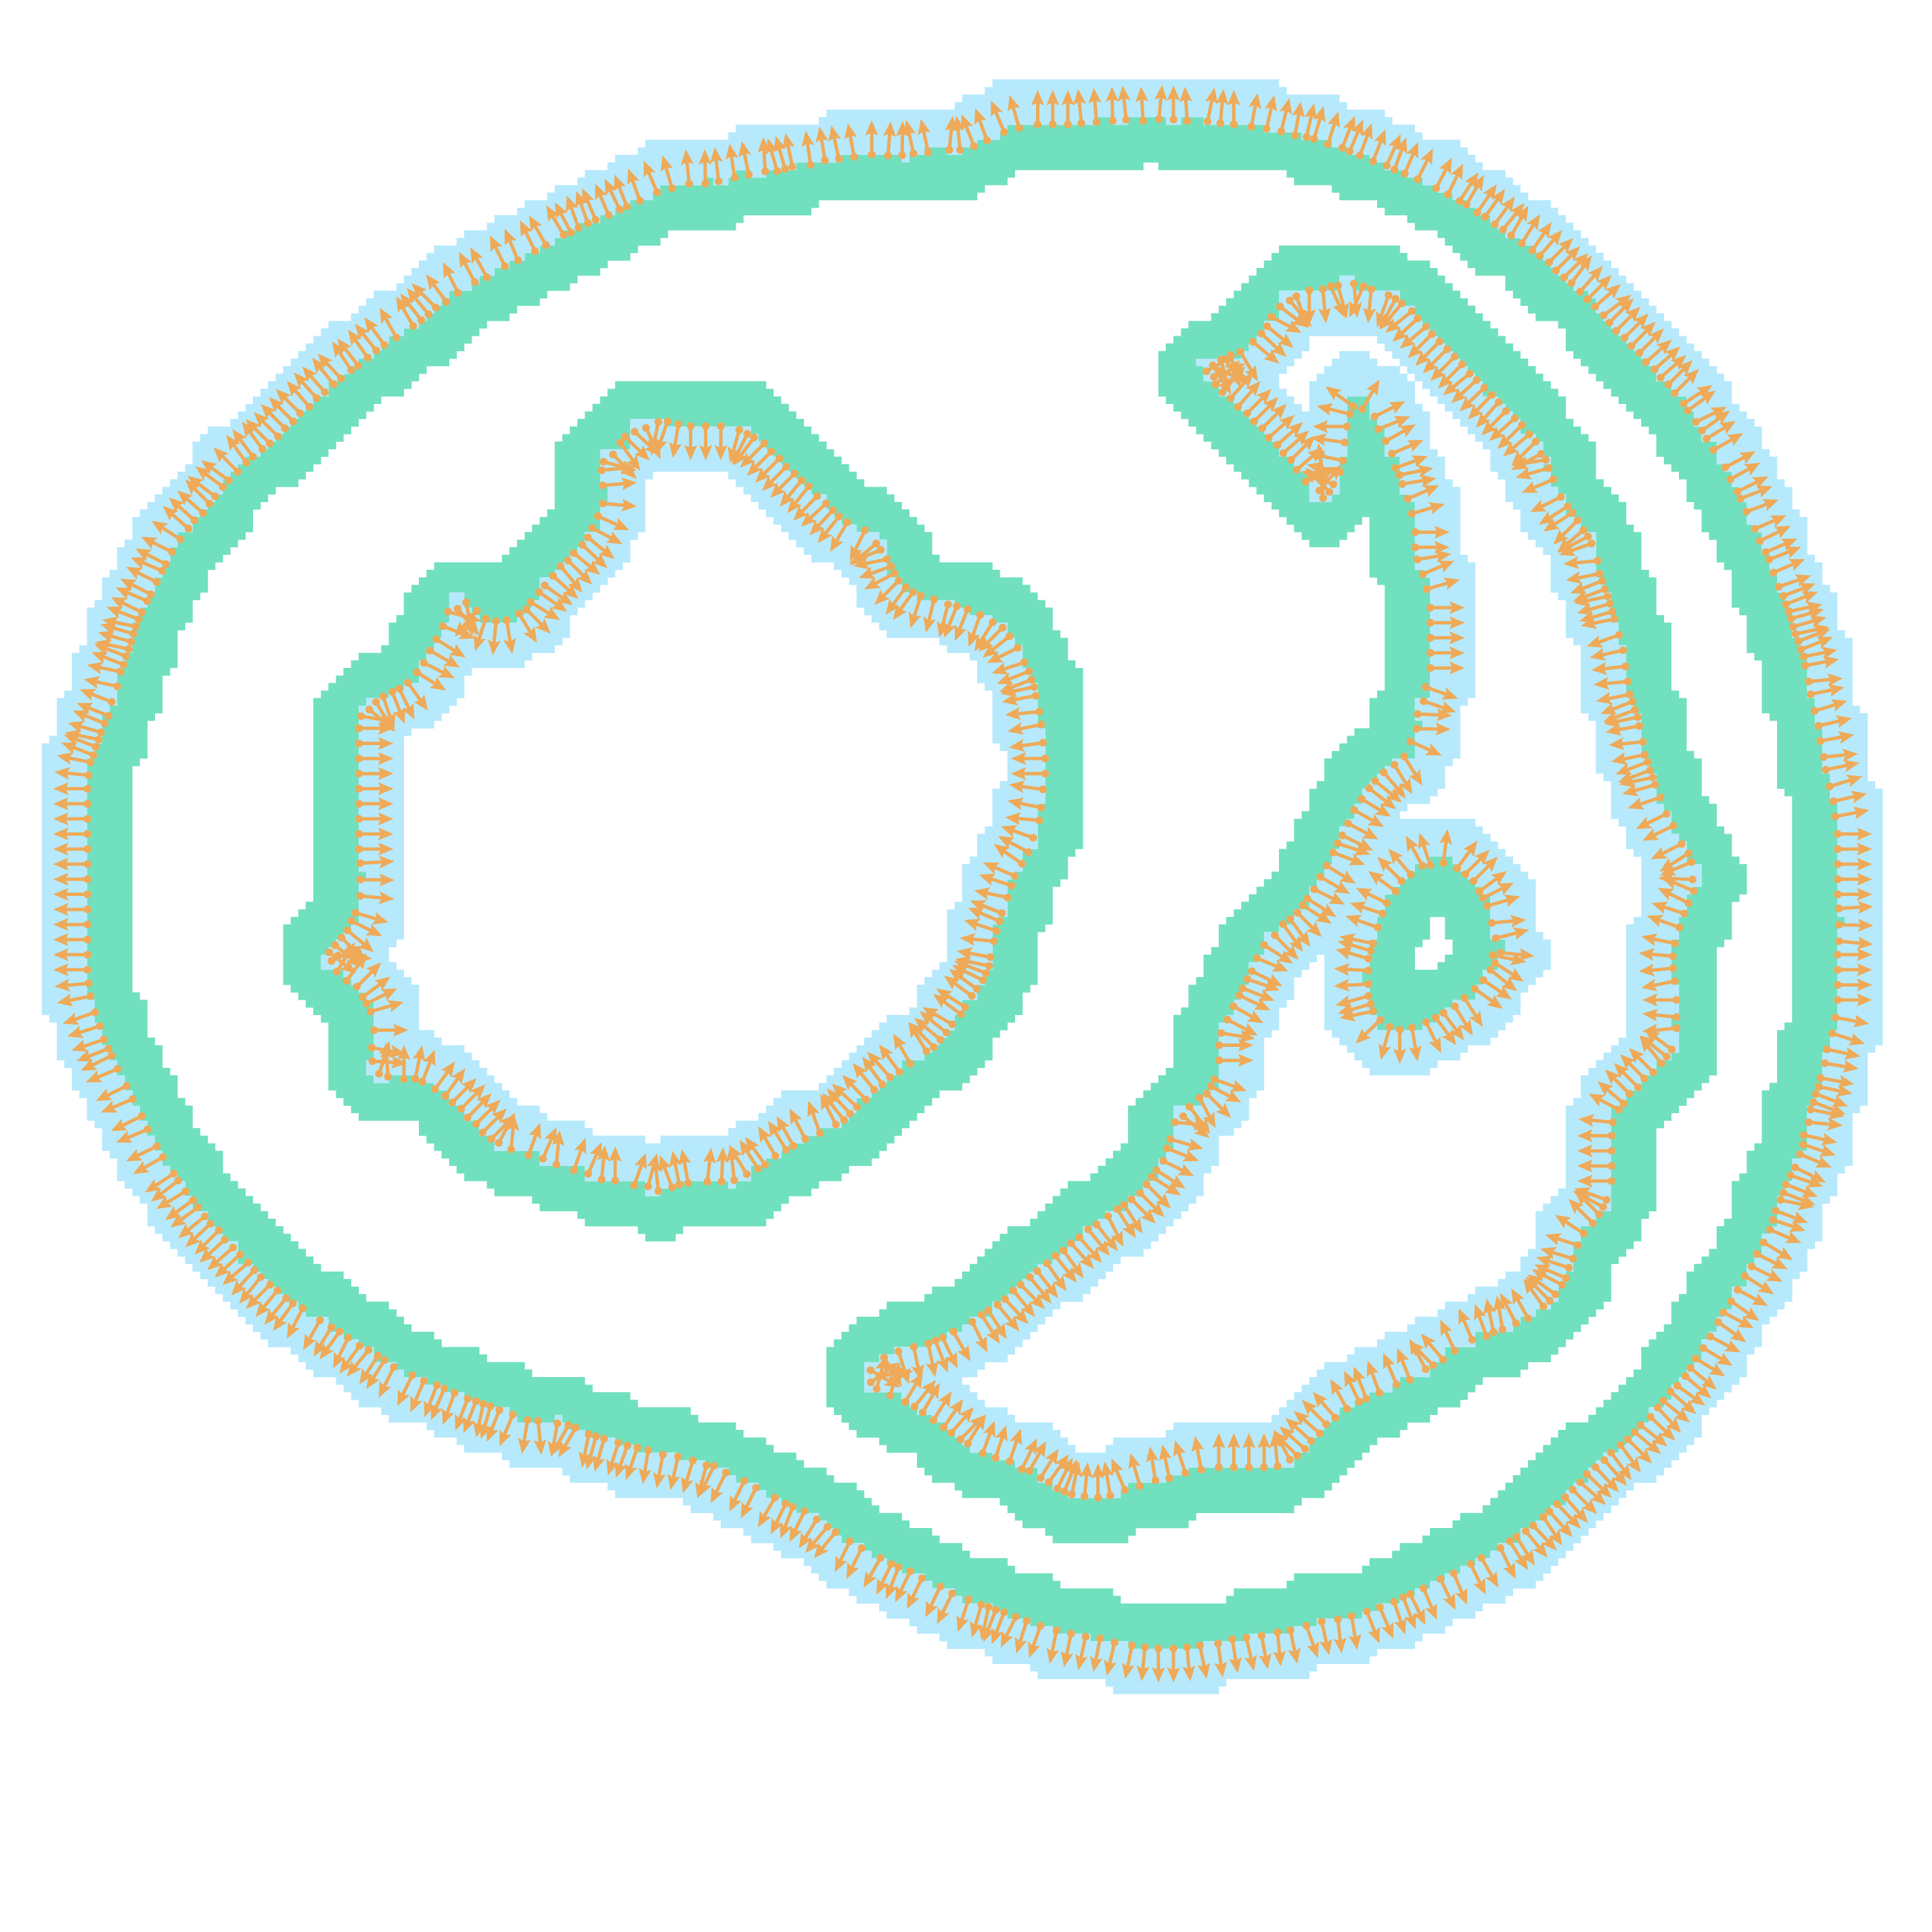
\includegraphics[scale=0.47]{media/vv/a222.png}
\label{fig:d2dvor2}}
\subfigure[]{%
		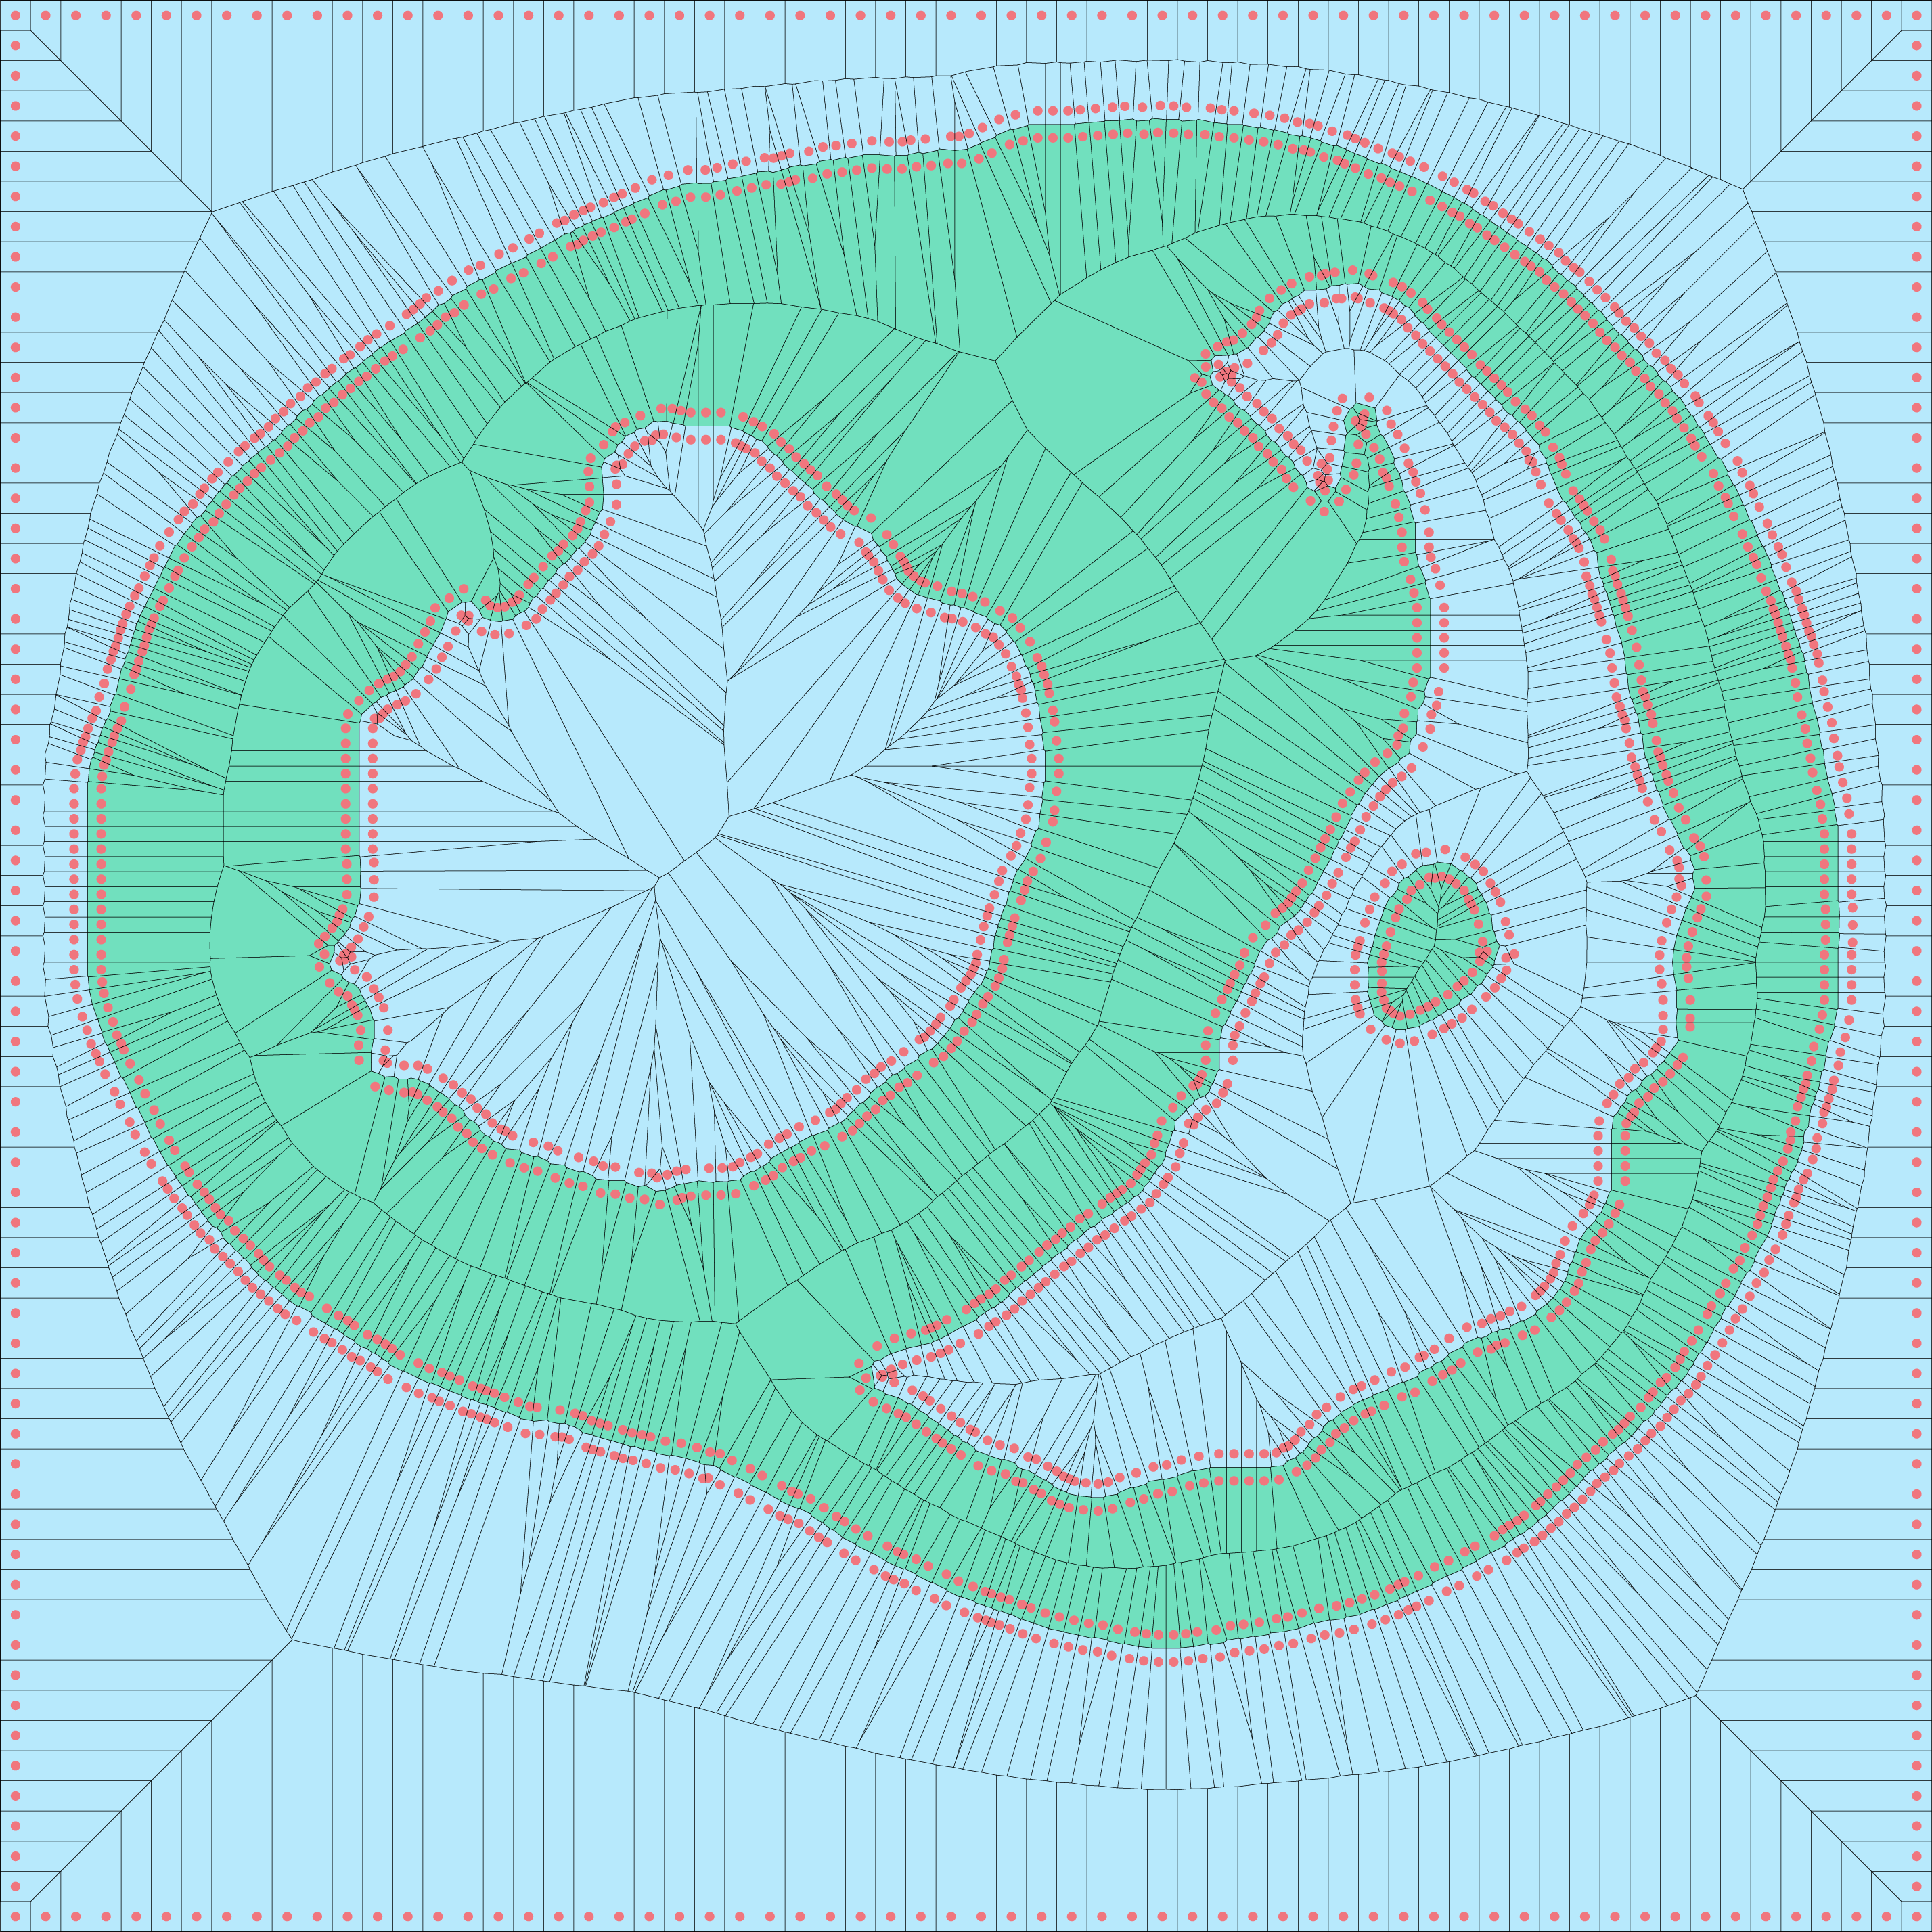
\includegraphics[scale=0.47]{media/vv/a333.png}
\label{fig:d2dvor3}}
%\subfigure[]{%
%		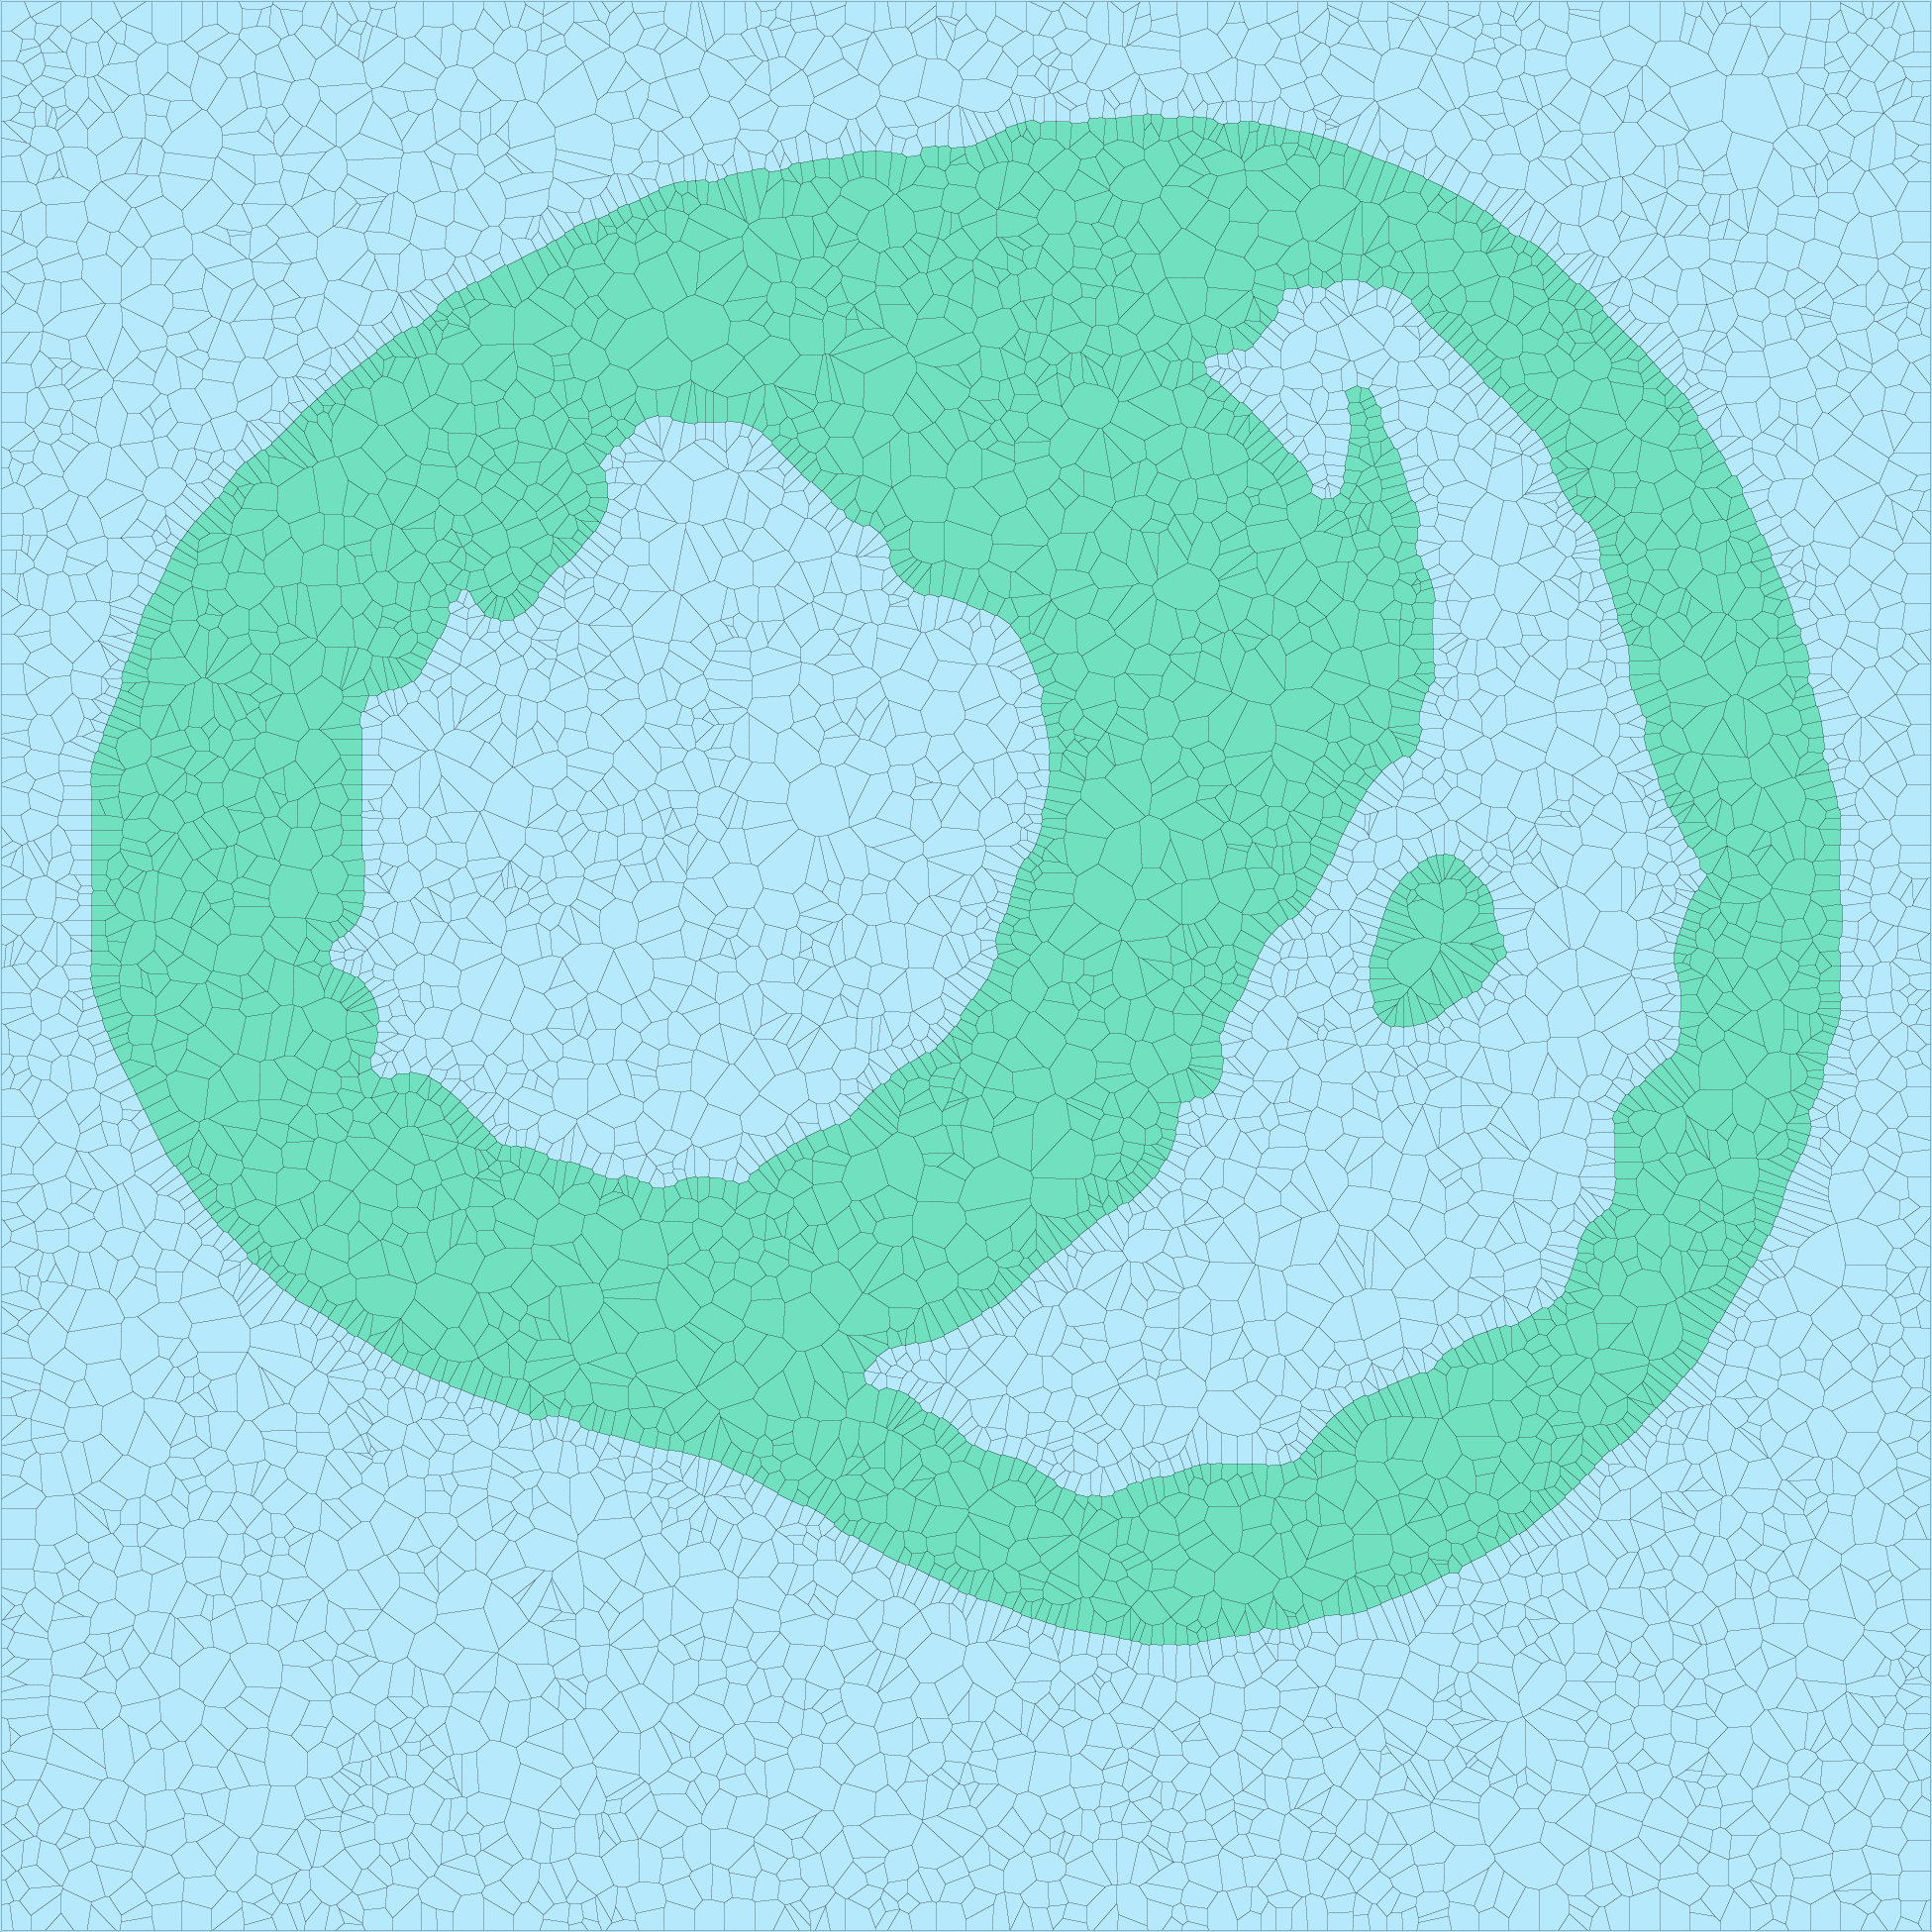
\includegraphics[scale=0.4]{media/vv/a4.png}
%\label{fig:d2dvor4}}
%
\caption{(a) Segmented image of 2D slice of \textit{ex vivo} canine heart (image mask generated from MRI data from Cardiovascular Research Grid~\cite{cvgg}), (b) resulting point cloud, and (c) Voronoi site placement and subsequent Voronoi partitioning and surface extraction. Point cloud and Voronoi sites are coarser than is typical for illustration purposes.}
\label{fig:d2dvor}
\end{figure}

\subsubsection{Surface Extraction and Cleanup}

The b-rep is extracted from the Voronoi partition as the set of facets that share Voronoi sites of differing material type. An additional step is performed, however, to mitigate undesired ``crosstalk'' facets caused by Voronoi partitioning of neighboring site pairs. ``Good facets'' are identified as those facets whose Voronoi sites belong to a site pair originating from the same point and normal, while ``bad facets'' are those facets whose Voronoi sites originate from two different points in the point cloud. For surfaces with small curvature, the total area of the good facets is vastly greater than that of the bad facets. Nonetheless, the existence of bad facets causes a stair-stepping feature in the resulting surface that is undesirable. \\ \\
%
These artifacts are addressed as follows: ``bad edges'' are identified as those edges that share two bad facets. Networks of connected bad edges are identified, and each network is collapsed to a point (see \figref{cross1}). For surfaces with a small amount of curvature, no bad edges are connected, and thus each is independently collapsed. Any good facet that is connected to a network of bad edges is modified to connect to the new collapsed point. Good facets are subsequently triangulated to maintain planarity following the collapse of bad edges. The sequence is demonstrated for an \textit{ex vivo} human heart example in~\figref{cross2}. \\

\begin{figure}[b!]
\centering
\subfigure[]{%
		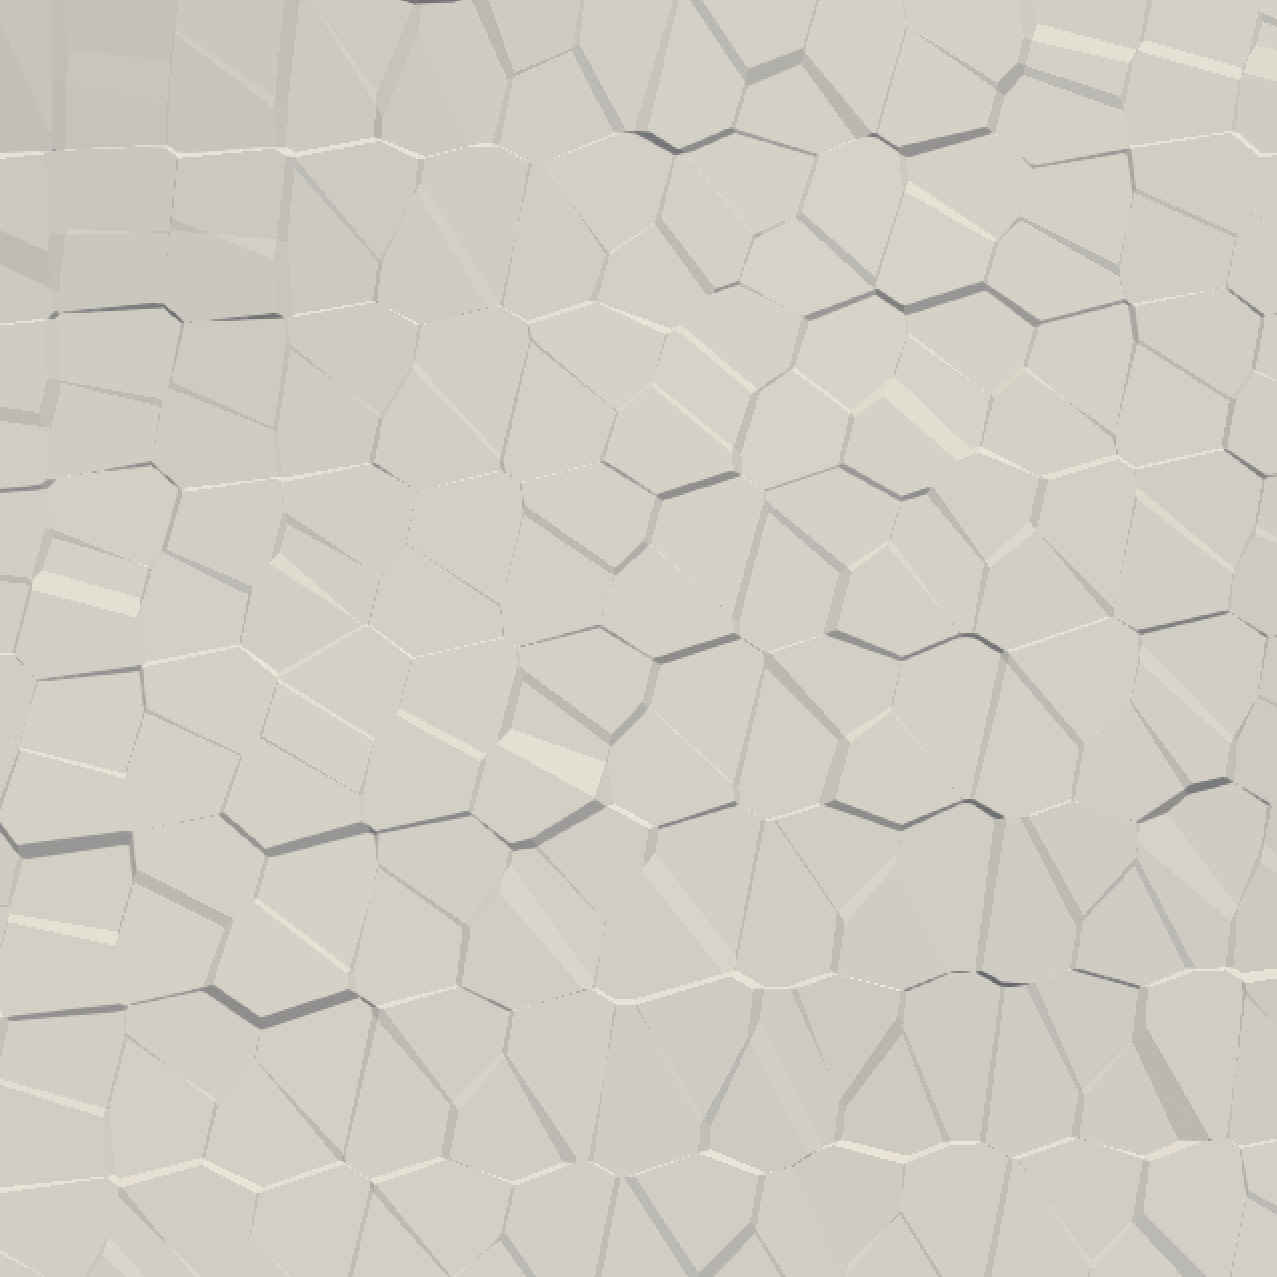
\includegraphics[scale=0.09]{media/2-shabaka/3-clean-zoom/1-init-zoom.png}
\label{fig:cross1-1}}	
\subfigure[]{%
		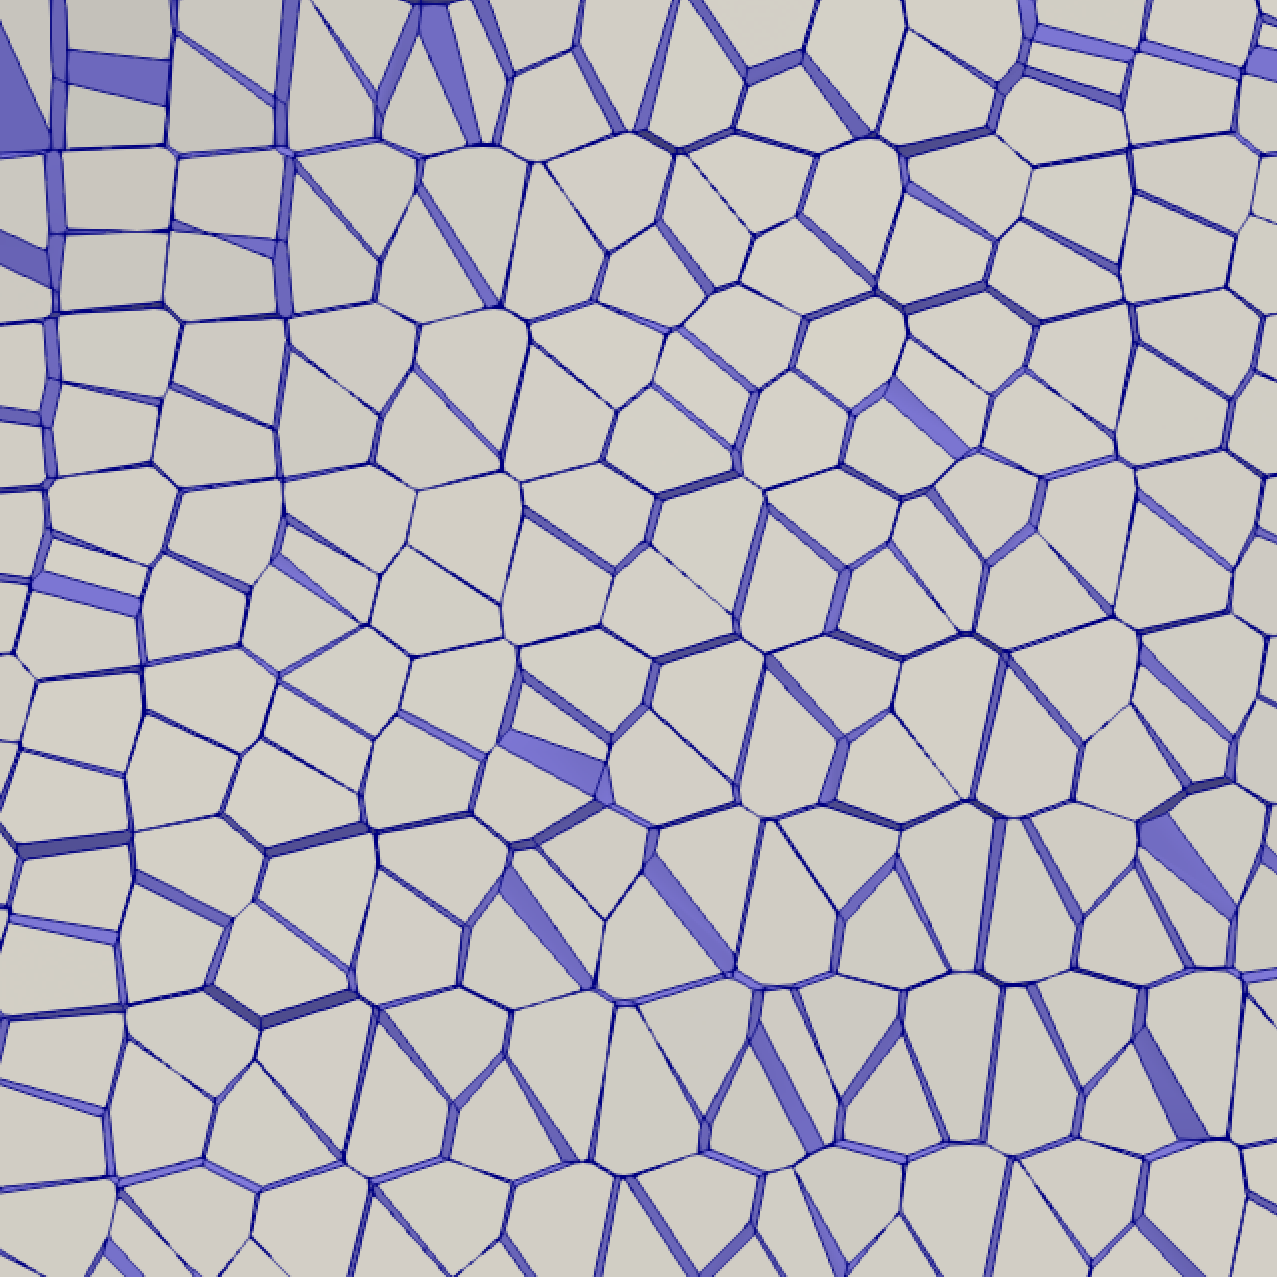
\includegraphics[scale=0.09]{media/2-shabaka/3-clean-zoom/2-badfacets-zoom.png}
\label{fig:cross1-2}}
\subfigure[]{%
		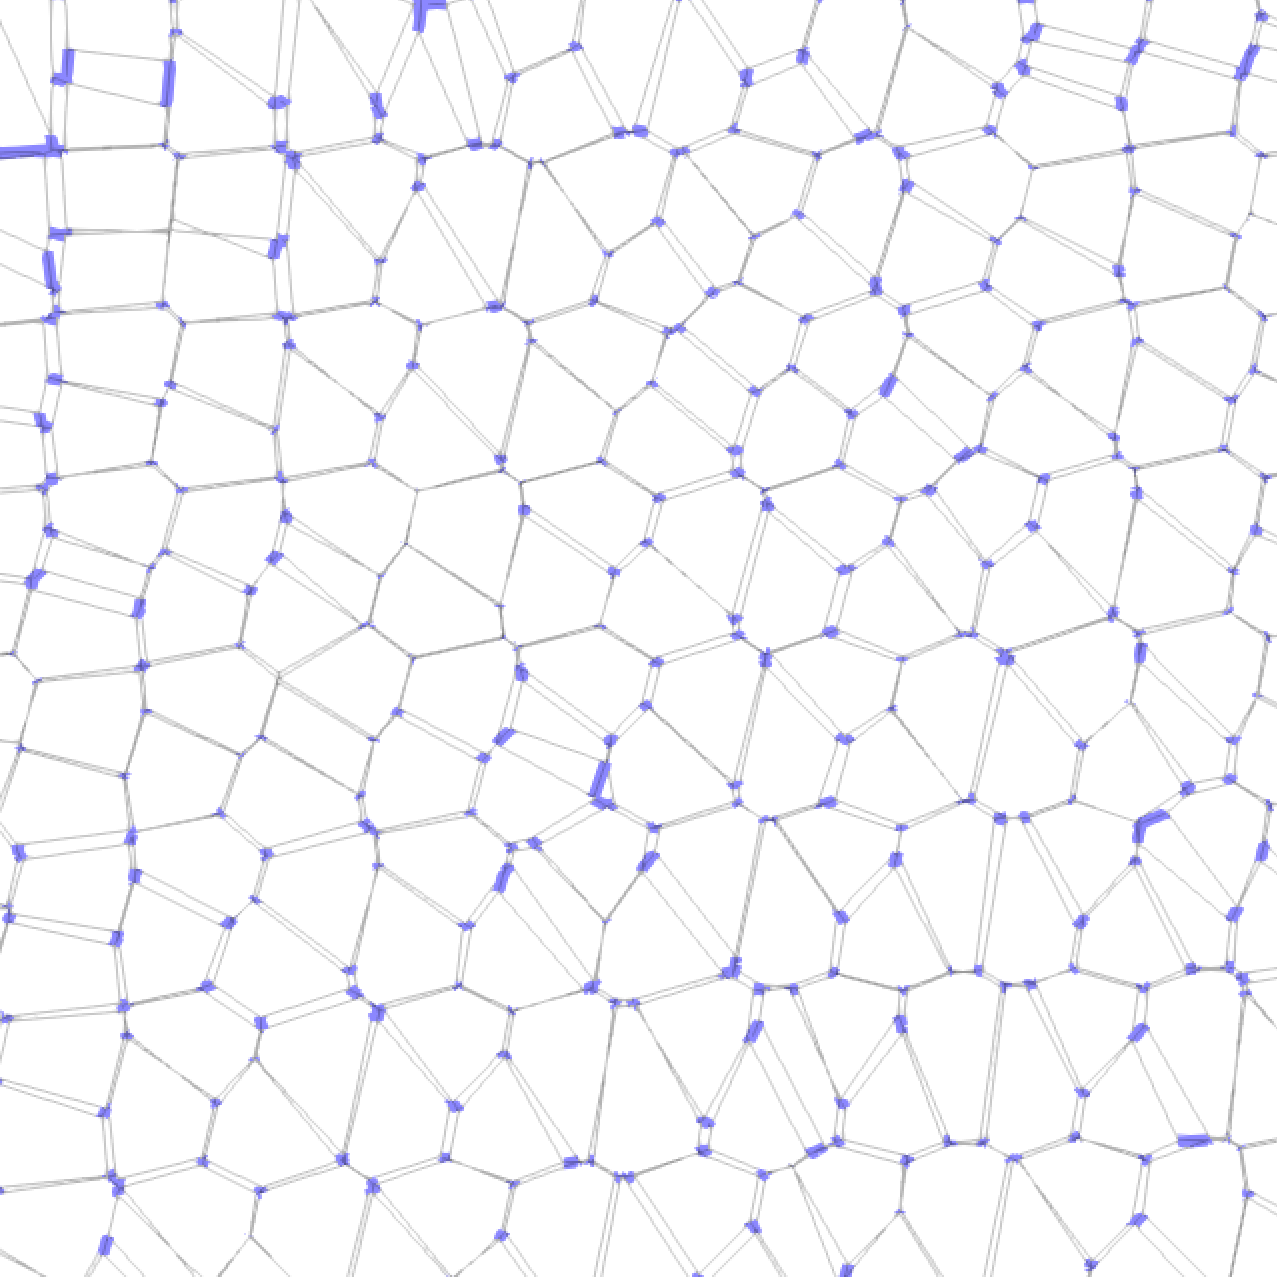
\includegraphics[scale=0.09]{media/2-shabaka/3-clean-zoom/3-badsegs-zoom.png}		
\label{fig:cross1-3}}
\subfigure[]{%
		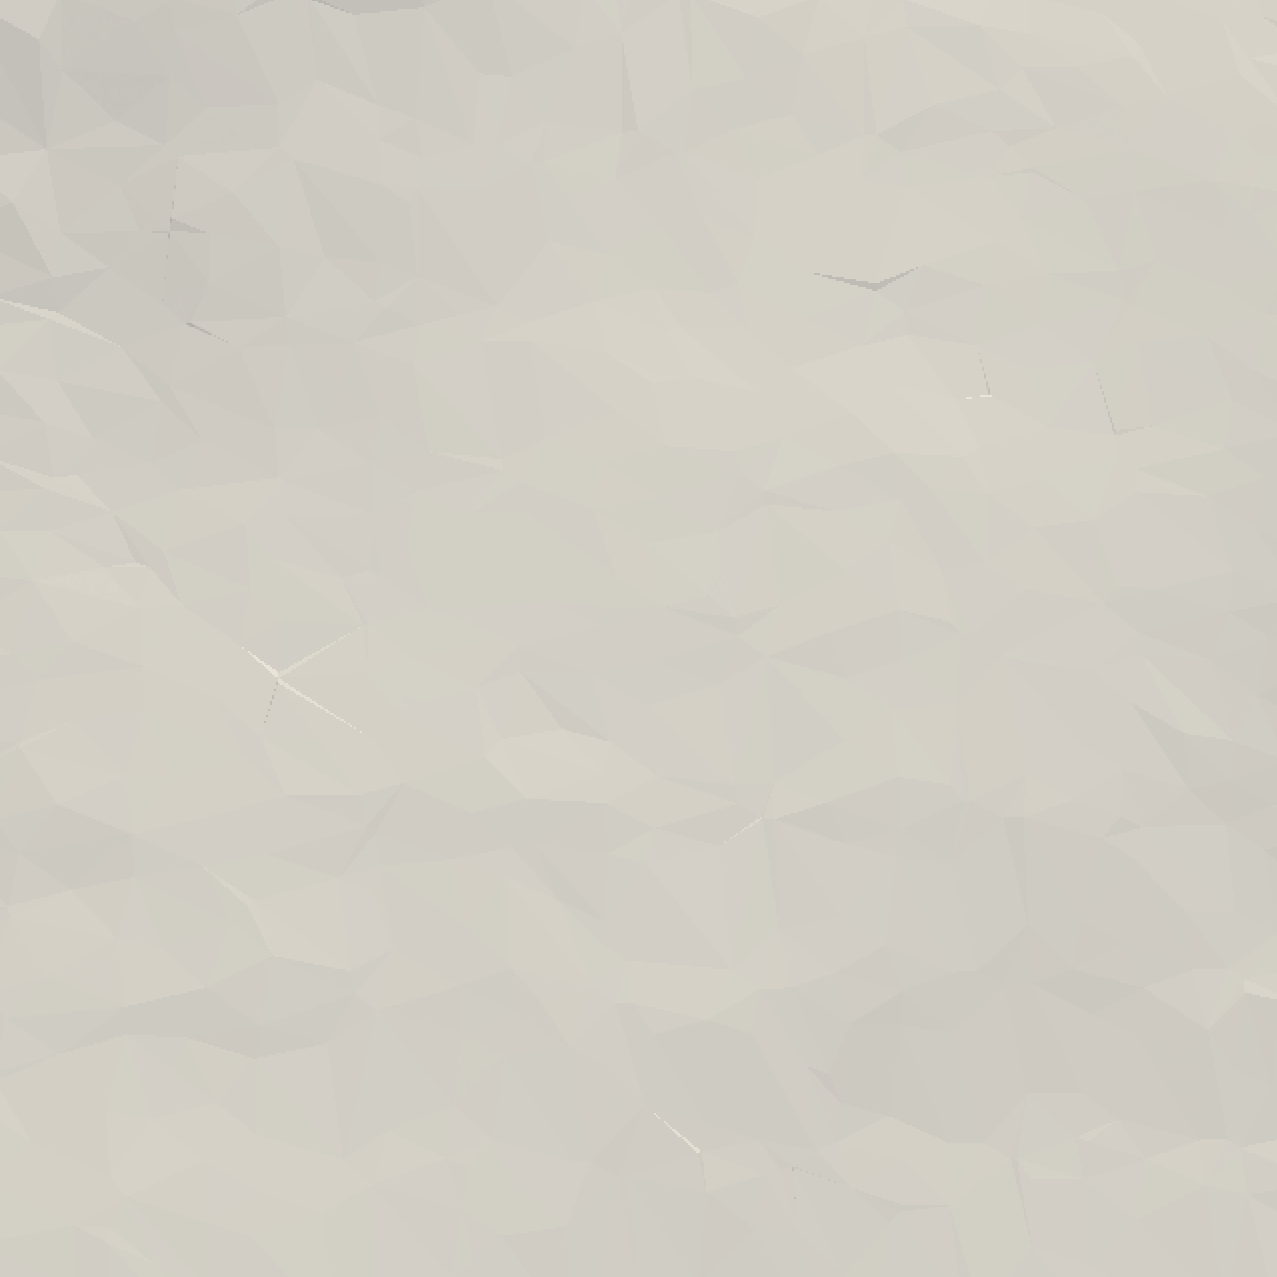
\includegraphics[scale=0.09]{media/2-shabaka/3-clean-zoom/4-fine-zoom.png}
\label{fig:cross1-4}}				
%
\caption{Cleanup of undesirable crosstalk facets for a surface patch: (a) initial surface following Voronoi-based surface reconstruction, (b) identification of crosstalk facets (purple), (c) identification of edges to be collapsed (purple), and (d) final cleaned surface.}
\label{fig:cross1}
\end{figure}

\begin{figure}[b!]
\centering
\subfigure[]{%
		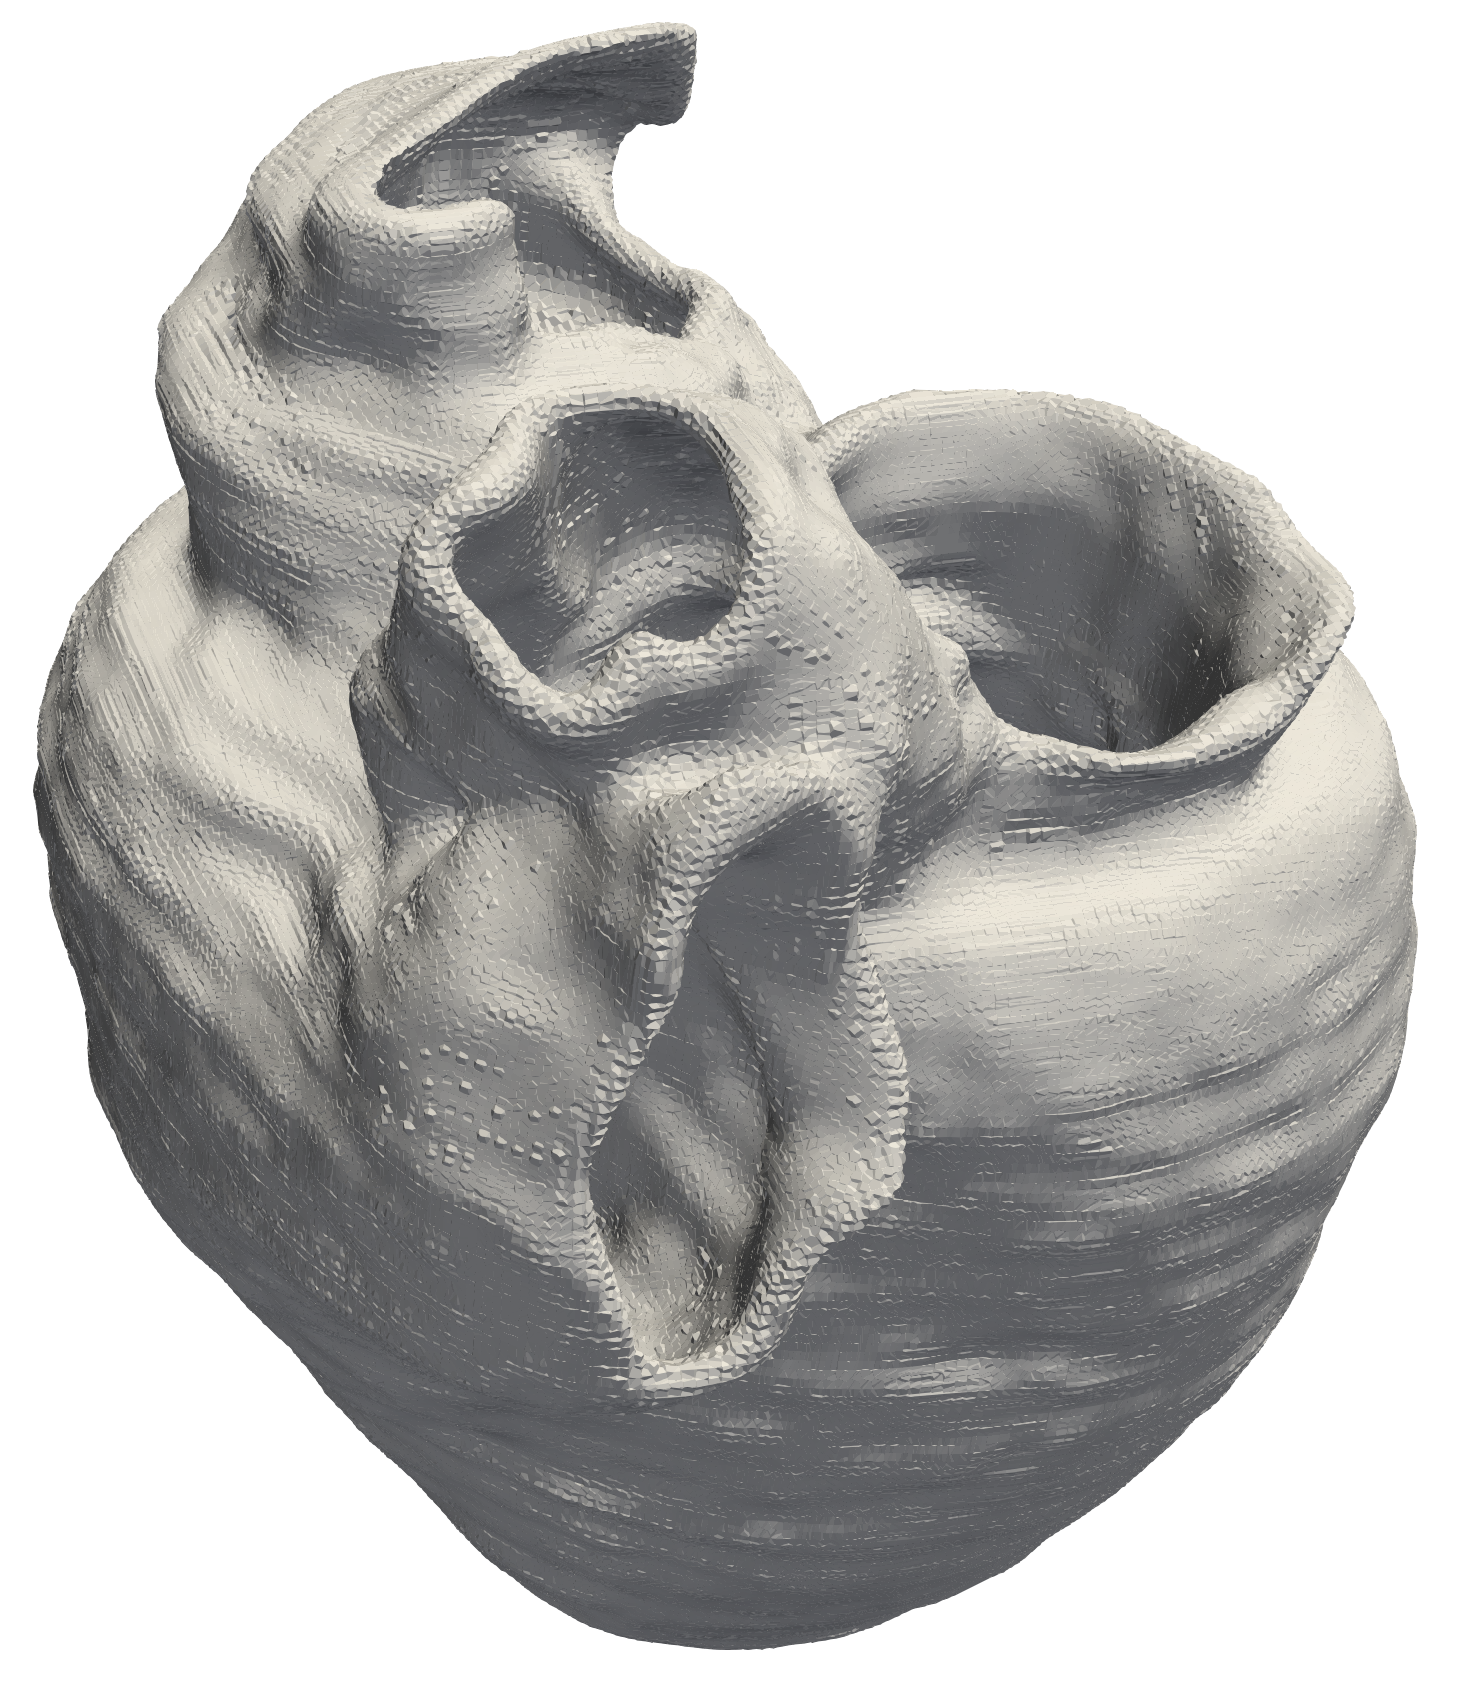
\includegraphics[scale=0.08]{media/2-shabaka/4-clean/1-init.png}
\label{fig:cross2-1}}		
\subfigure[]{%
		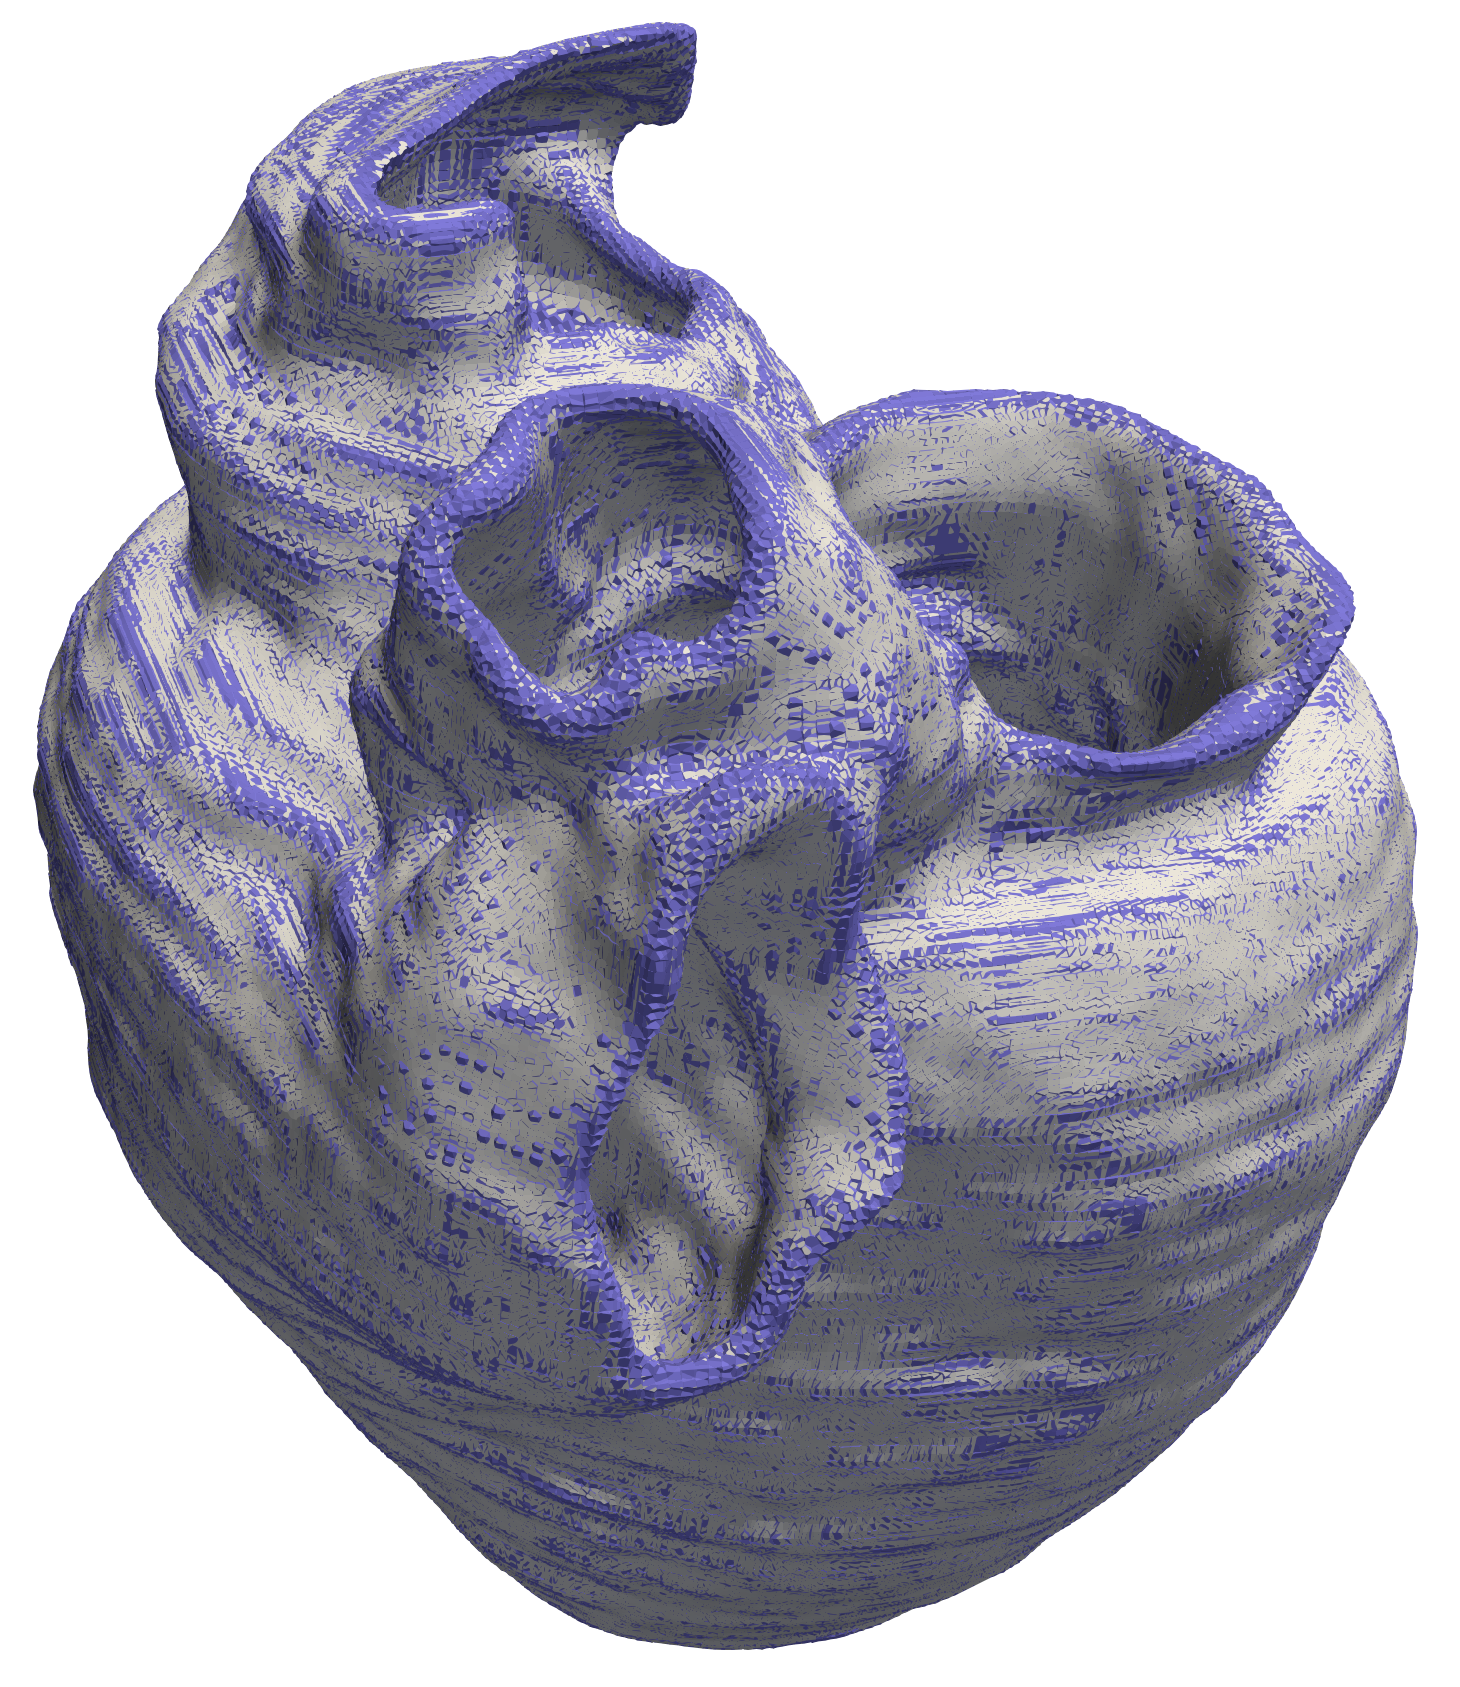
\includegraphics[scale=0.08]{media/2-shabaka/4-clean/2-badfacets.png}
\label{fig:cross2-2}}		
\subfigure[]{%
		\includegraphics[scale=0.08]{media/2-shabaka/snapsegs-v2.png}	
\label{fig:cross2-3}}						
\subfigure[]{%
		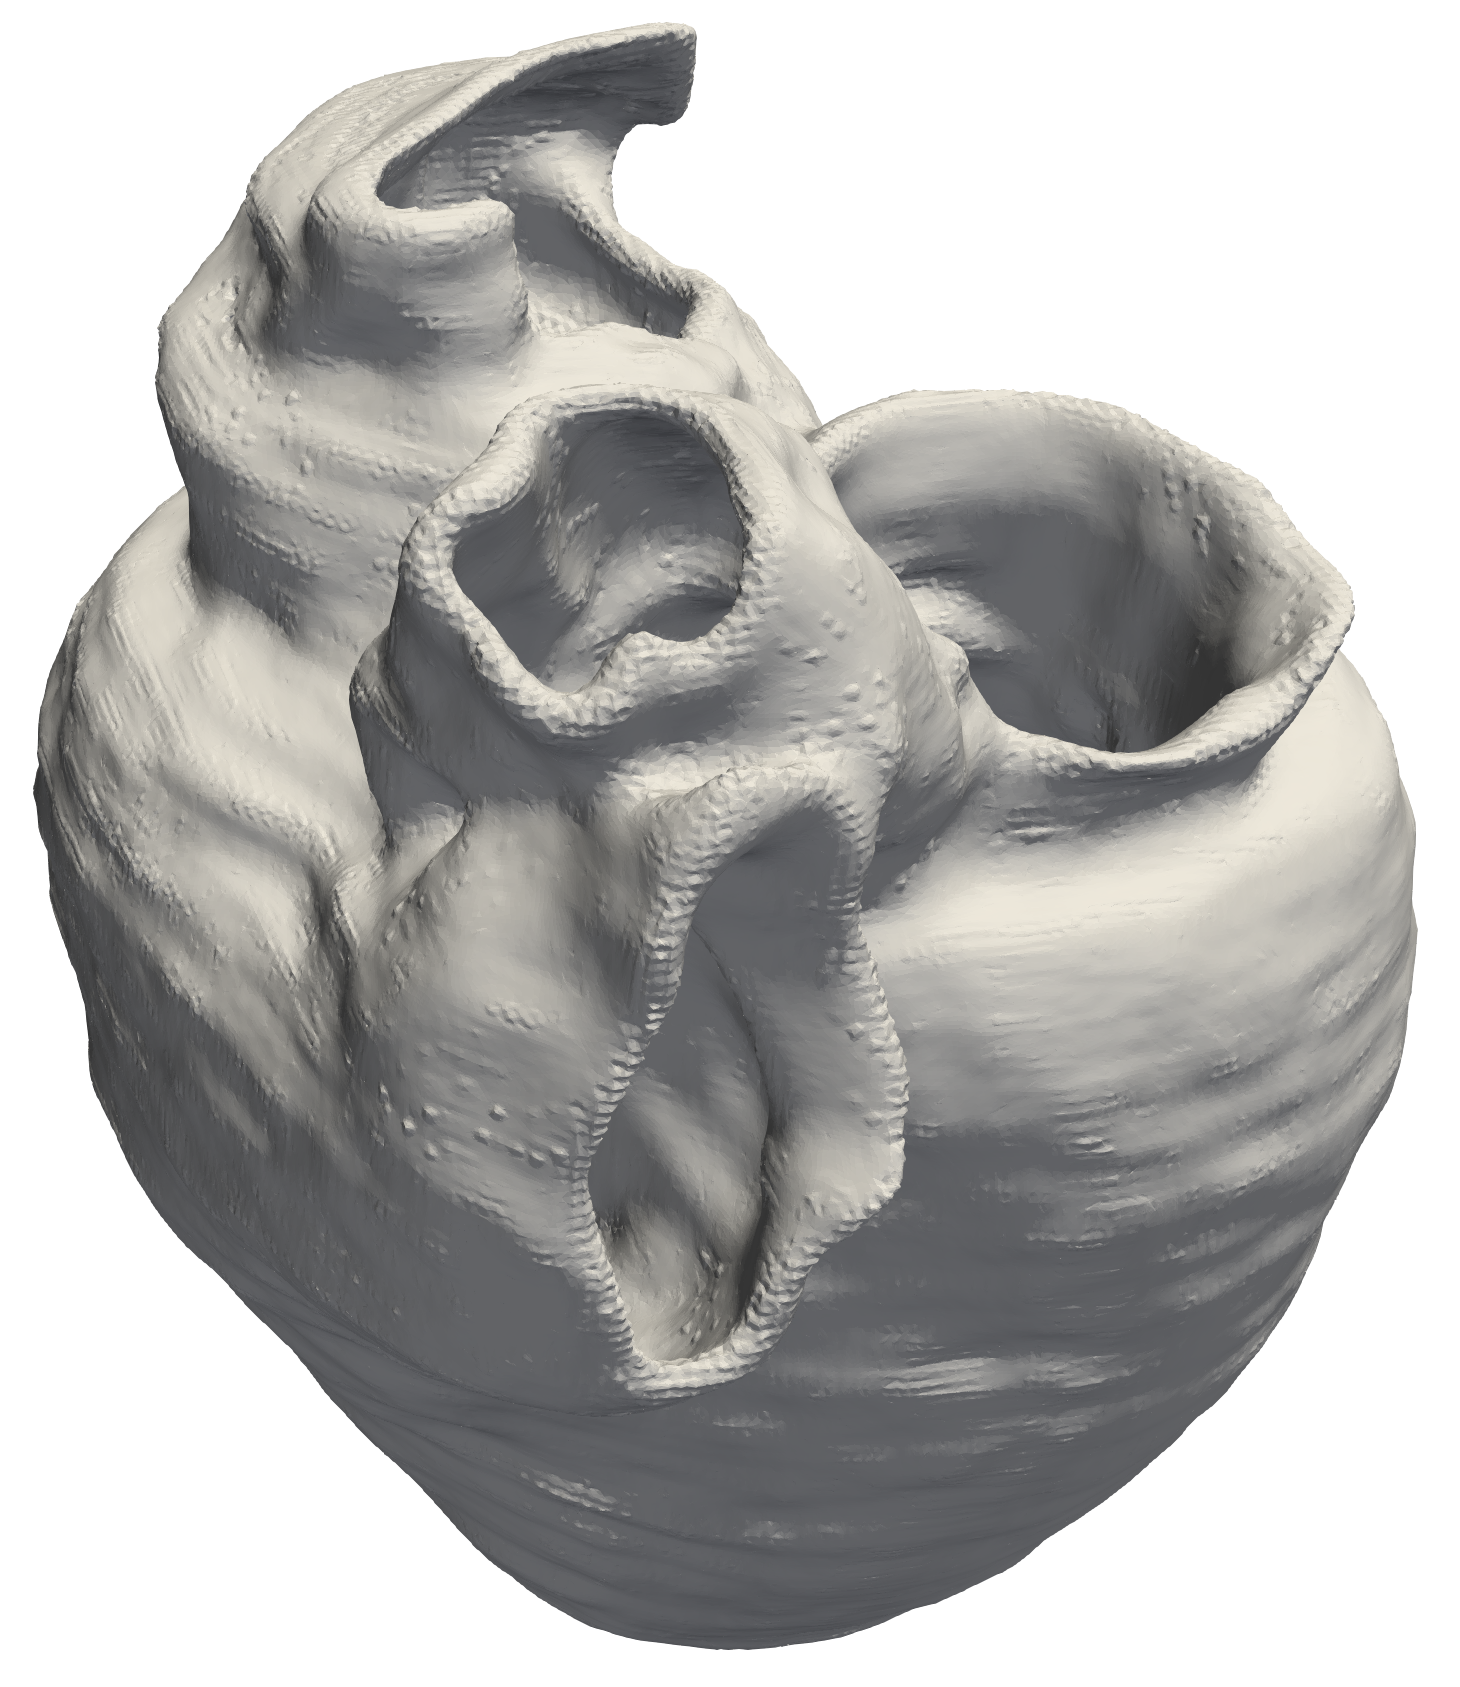
\includegraphics[scale=0.08]{media/2-shabaka/4-clean/4-fine.png}		
\label{fig:cross2-4}}		
%
\caption{Cleanup of undesirable crosstalk facets for surface of \textit{ex vivo} human heart (corresponding image mask generated from MRI data from Cardiovascular Research Grid~\cite{cvgg}): (a) initial surface following Voronoi-based surface reconstruction, (b) identification of crosstalk facets (purple), (c) identification of edges to be collapsed (purple), and (d) final cleaned surface.}
\label{fig:cross2}
\end{figure}
\noindent For the vast majority of bad-edge networks, the collapsing technique results in a smoother surface that remains closed and manifold. For regions of high curvature, there are rare cases in which collapsing a network may cause the surface to become non-manifold. Accordingly, the topologies of those particular bad-edge networks are not collapsed in order to preserve the manifold property. The current approach is thus unable to completely alleviate the issue of crosstalk facets in regions of high curvature. Fortunately, these remaining artifacts are small enough that the ensuing decimation step removes them. \\ \\
%
Regions of high curvature, or even sharp corners and edges, can be addressed via an enhancement of the point-cloud-generation algorithm described previously. The enhancement involves including additional templates when locally approximating boundaries, such that more than two Voronoi sites are generated for each sampling window. For example, three Voronoi sites can be used to produce an edge, and four sites can be used to produce a corner. In this manner, multiple boundary point/normal pairs for a single sampling window would naturally occur to reconstruct regions of high curvature.

\subsubsection{Surface Decimation and Smoothing}

Surface \textit{decimation} is performed to reduce the surface mesh to a practical resolution without significantly changing the geometry. The philosophy is to make use of as much information as is available to construct a surface mesh of the highest fidelity possible, and only then to address the practical consideration of mesh resolution for simulation or other purposes. The challenge, then, becomes decimating to a degree that does not result in undesired feature loss.  For purposes of the present algorithm, decimation is performed using the code \textit{ACVD}~\cite{valette_2004, valette_2008}, which clusters vertices and triangles to generate a coarser surface mesh whose resulting triangles exhibit desirable aspect ratios. The approach does not preserve sharp edges or corners, however; feature-preserving decimation is still very much an active topic of research. \textcolor{purple}{It is noted that, in the subsequent Performance Assessment section, this decimation step does not introduce any measurable error in reconstructing a spherical image mask for either marching cubes, screened Poisson, or the proposed method.} As is typical in b-rep construction algorithms, we apply smoothing as a final step. Specifically, Taubin smoothing~\cite{taubin1995signal, taubin_1995} is employed to produce smooth surfaces without significant loss of volume. \textcolor{purple}{The smoothing step is performed using the implemented of Taubin smoothing within \textit{Meshlab}~\cite{meshlab}}.

\subsubsection{\textcolor{purple}{Parameter Selection}}

Results of the entire surface generation procedure are shown in~\figref{shabakaseq} for an \textit{ex vivo} human heart example~\cite{cvgg}. The optimal parameters identified for robust surface generation are shown in~\tabref{Mod5}. \textcolor{purple}{The decimation and smoothing parameters were selected within \textit{ACVD} and \textit{Meshlab}, respectively.} The algorithm was rigorously tested with these parameters to produce closed, manifold, watertight surfaces for a wide variety of examples, as is shown in the next section. \\

\begin{table}[h!]
 \centering
   \begin{tabular}{|c||c|c|}
   \hline 
   \textbf{Variable} & \textbf{Description} & \textbf{Value} \\ \hline \hline
   $R_{\mathcal{W}}$ & window radius (in voxels) & 5 \\ \hline
   $d_{\mathcal{W}}$ & sampling distance between adjacent windows (in voxels) & 2 \\ \hline
   \multirow{2}{*}{$\overline{k}_{\mathcal{M}}$ \rule{0mm}{4mm}} & threshold for acceptable ratio of voxels in & \multirow{2}{*}{0.925} \\
   {} & window $\mathcal{W}$ belonging to material of interest & {} \\ \hline
   $\beta_0$ & weighting coefficient for error in zeroth polynomial moment & 0.5 \\ \hline
   $\beta_1$ & weighting coefficient for error in first polynomial moments & 0.3 \\ \hline   
   $\varepsilon$ & tolerance for minimization of function $\mathcal{F}$ & $10^{-14}$ \rule{0mm}{4mm} \\ \hline
   $\overline{\mathcal{F}}$ \rule{0mm}{4mm} & largest acceptable value of function $\mathcal{F}$ & $0.15$ \\ \hline
   \multirow{2}{*}{$b$} & distance between boundary normal and & \multirow{2}{*}{$1.1$} \\
   {} & corresponding Voronoi site pair (in voxels) & {} \\ \hline
   $\color{purple}{g}$ & \textcolor{purple}{gradation (decimation)} & $\color{purple}{0.5}$ \\ \hline
   $\color{purple}{s}$ & \textcolor{purple}{subsampling threshold (decimation)} & $\color{purple}{2}$ \\ \hline
   $\color{purple}{\lambda}$ & \textcolor{purple}{positive smoothing scale factor} & $\color{purple}{0.5}$ \\ \hline
   $\color{purple}{\mu}$ & \textcolor{purple}{negative smoothing scale factor} & $\color{purple}{-0.53}$ \\ \hline
   $\color{purple}{n_s}$ & \textcolor{purple}{number of smoothing steps} & $\color{purple}{10}$ \\ \hline
\end{tabular}
\caption{Optimal parameter values for b-rep generation.}
\label{tab:Mod5}
\end{table}
%%%%%%%%%%%%%%%%%%%%%%%%%%%%%%%%%%%%%%%%%%%%%%%
%%%%%%%%%%%%%%%%%%%%%%%%%%%%%%%%%%%%%%%%%%%%%%%
\subsection{\textcolor{purple}{Workflow Summary}}
\label{Workflow Summary}

\color{purple}
Text

\color{black}
\begin{figure}[]
\centering
\subfigure[]{%
		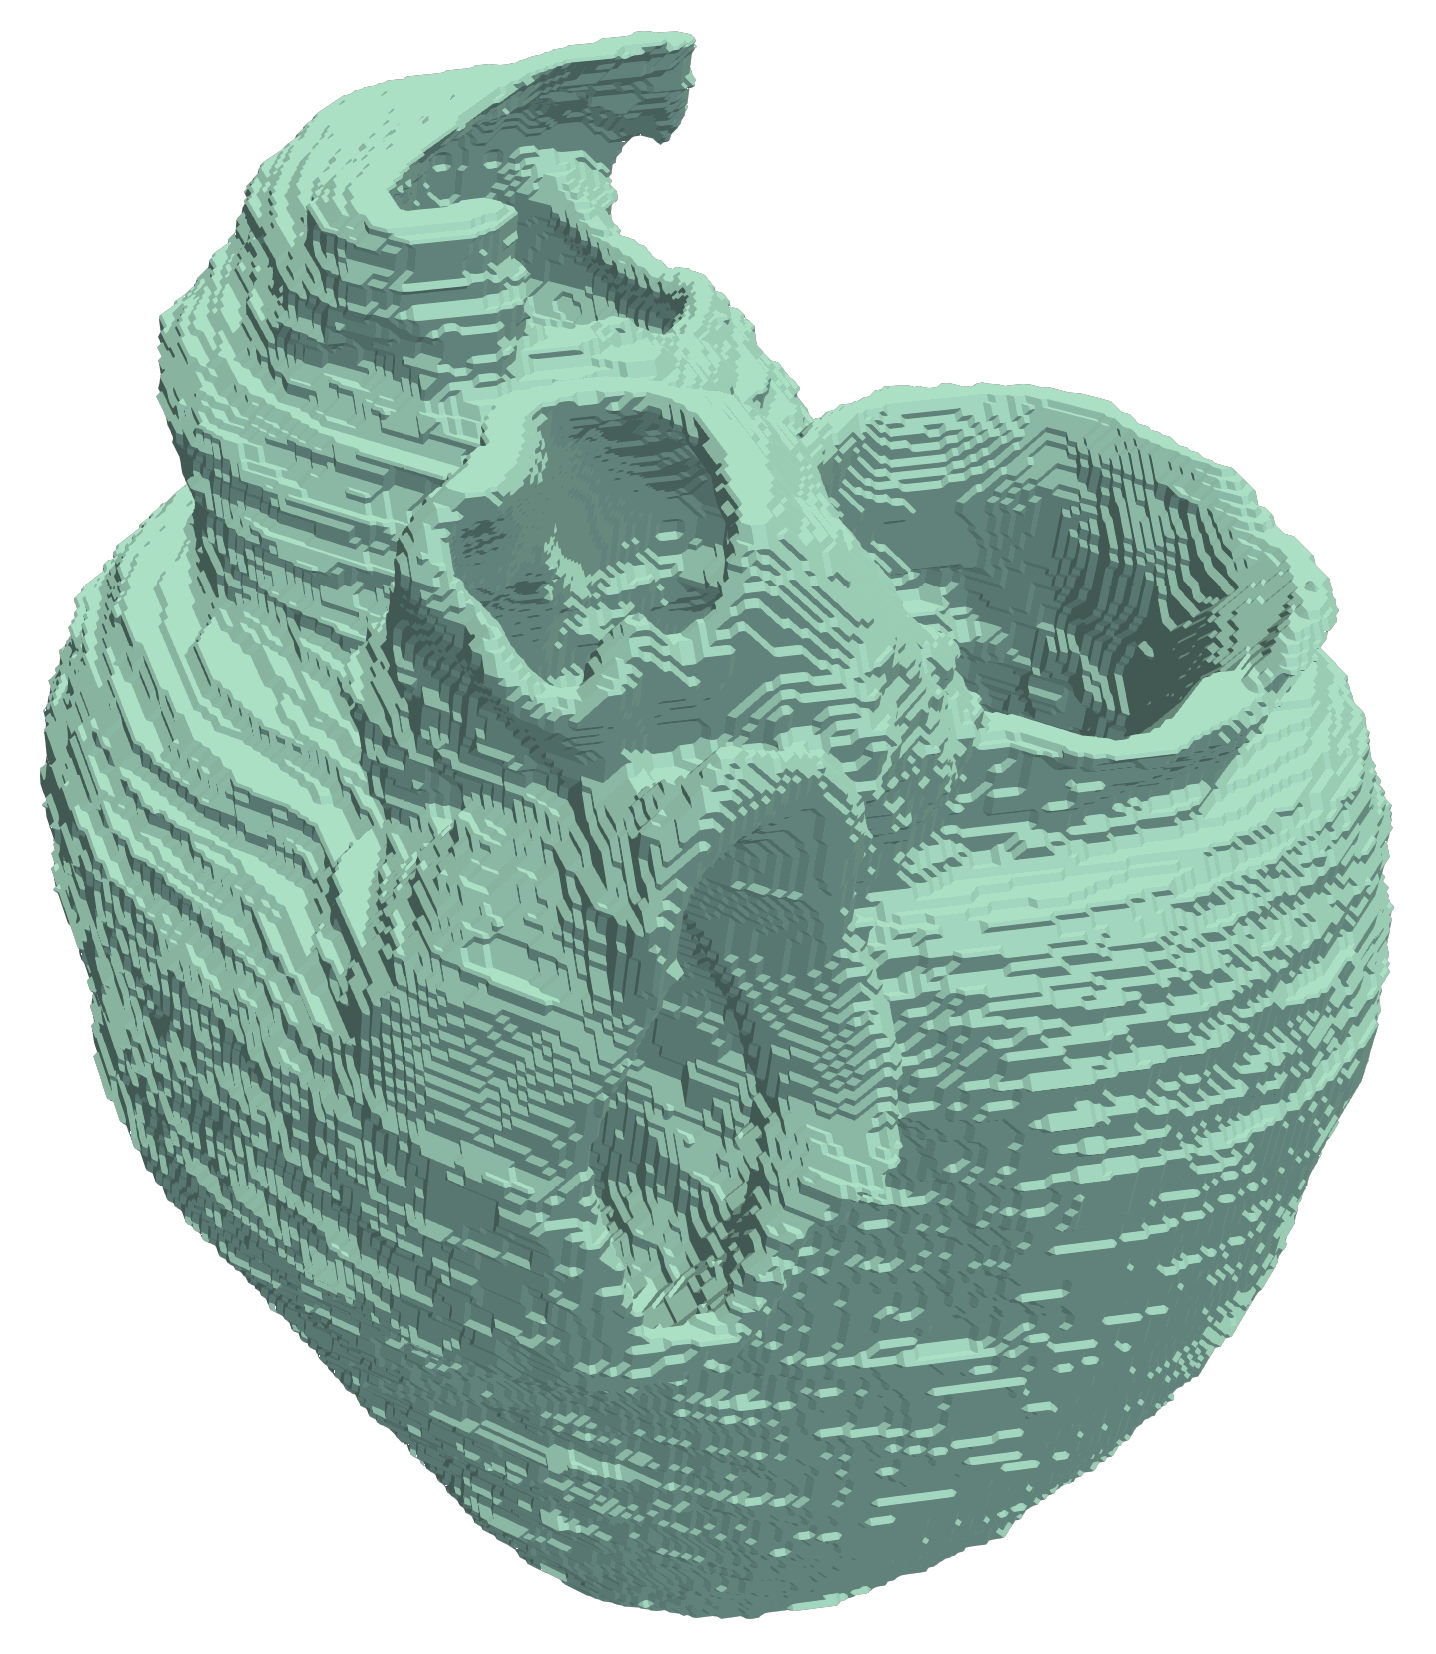
\includegraphics[scale=0.08]{media/2-shabaka/seg.png}
\label{fig:shabakaseq1}}
\subfigure[]{%
		\includegraphics[scale=0.08]{media/2-shabaka/normals.png}
\label{fig:shabakaseq2}}
\subfigure[]{%
		\includegraphics[scale=0.08]{media/2-shabaka/points.png}
\label{fig:shabakaseq3}}
\\
\subfigure[]{%
		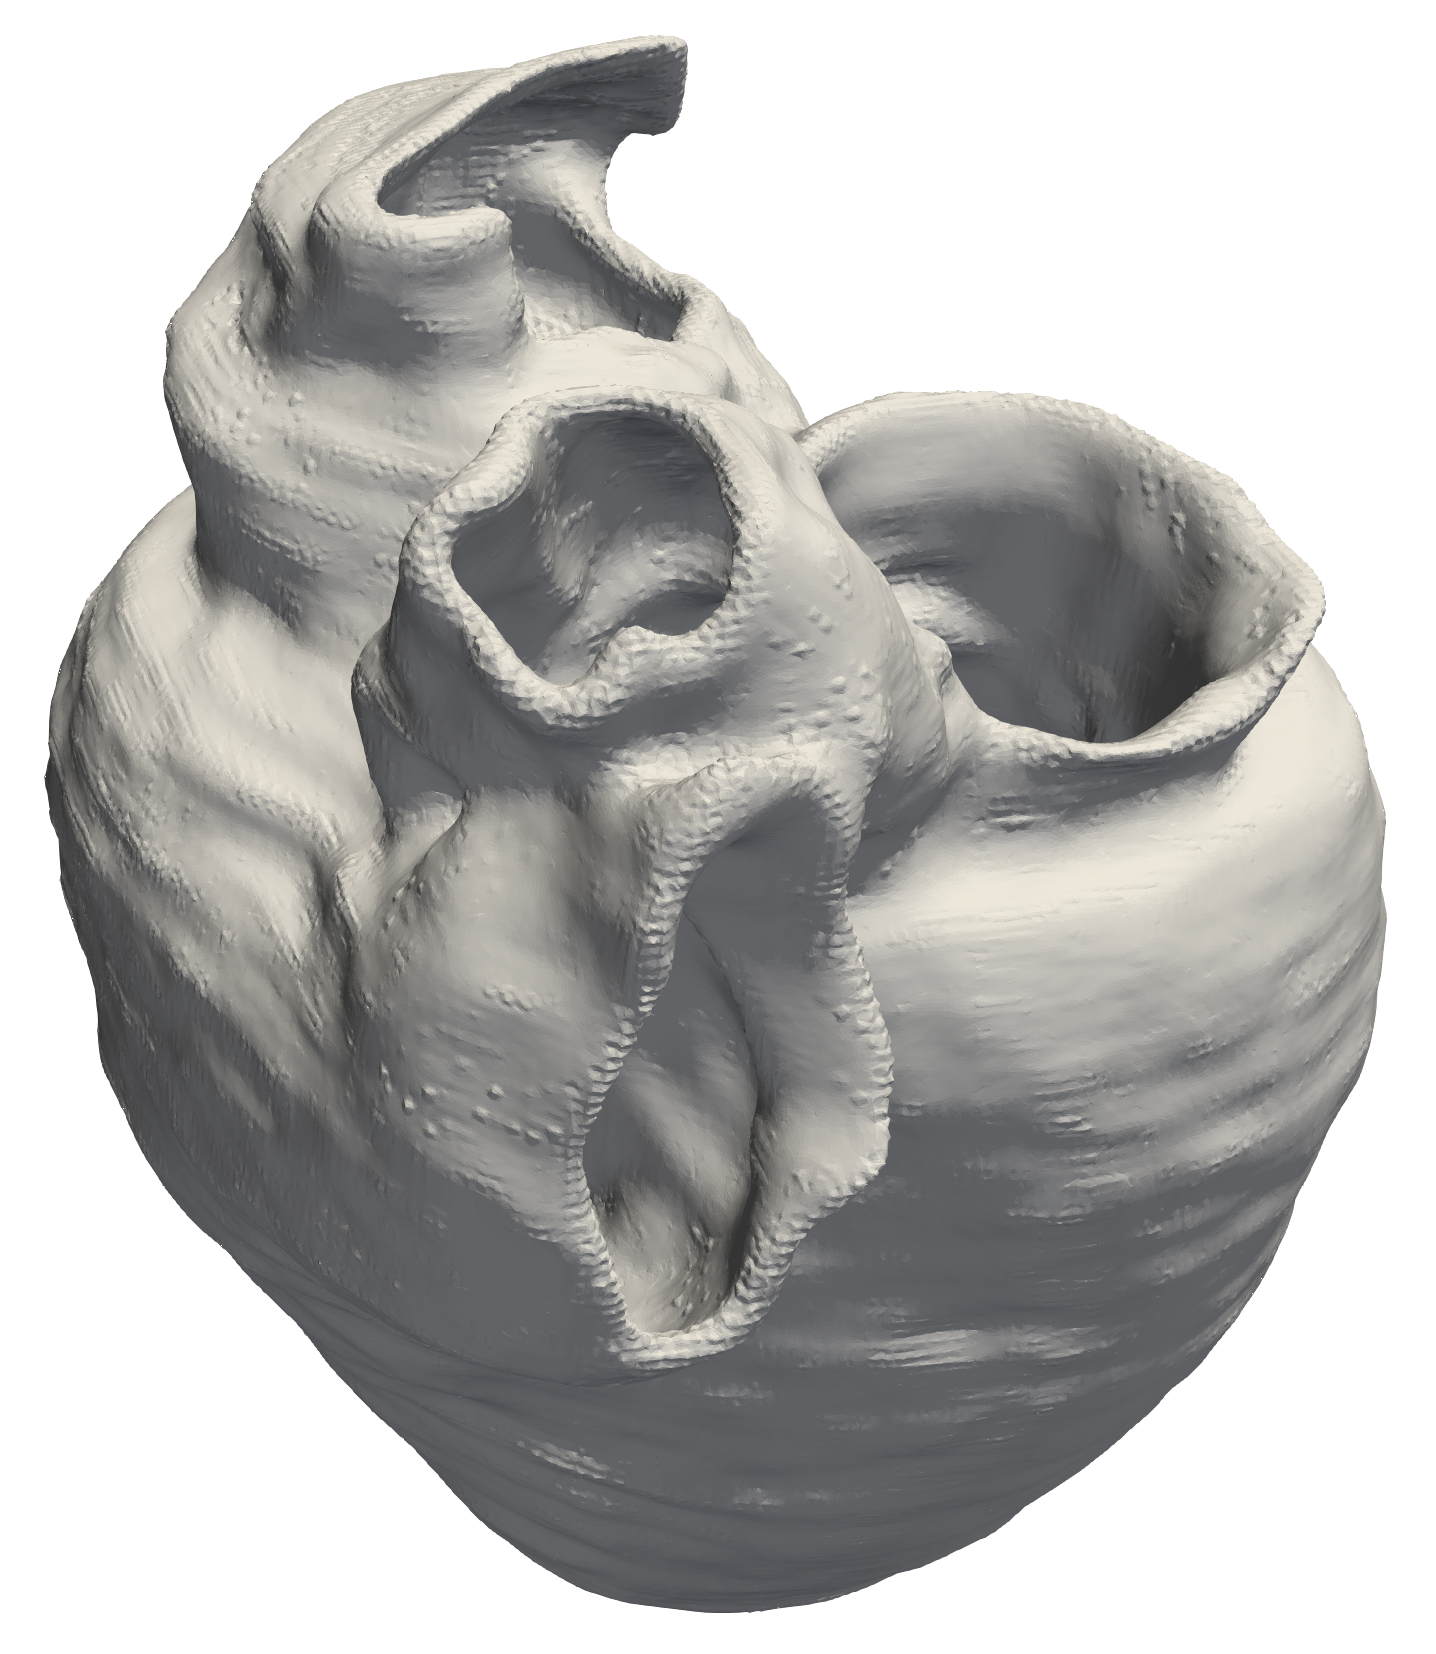
\includegraphics[scale=0.08]{media/2-shabaka/fine.png}
\label{fig:shabakaseq4}}
\subfigure[]{%
		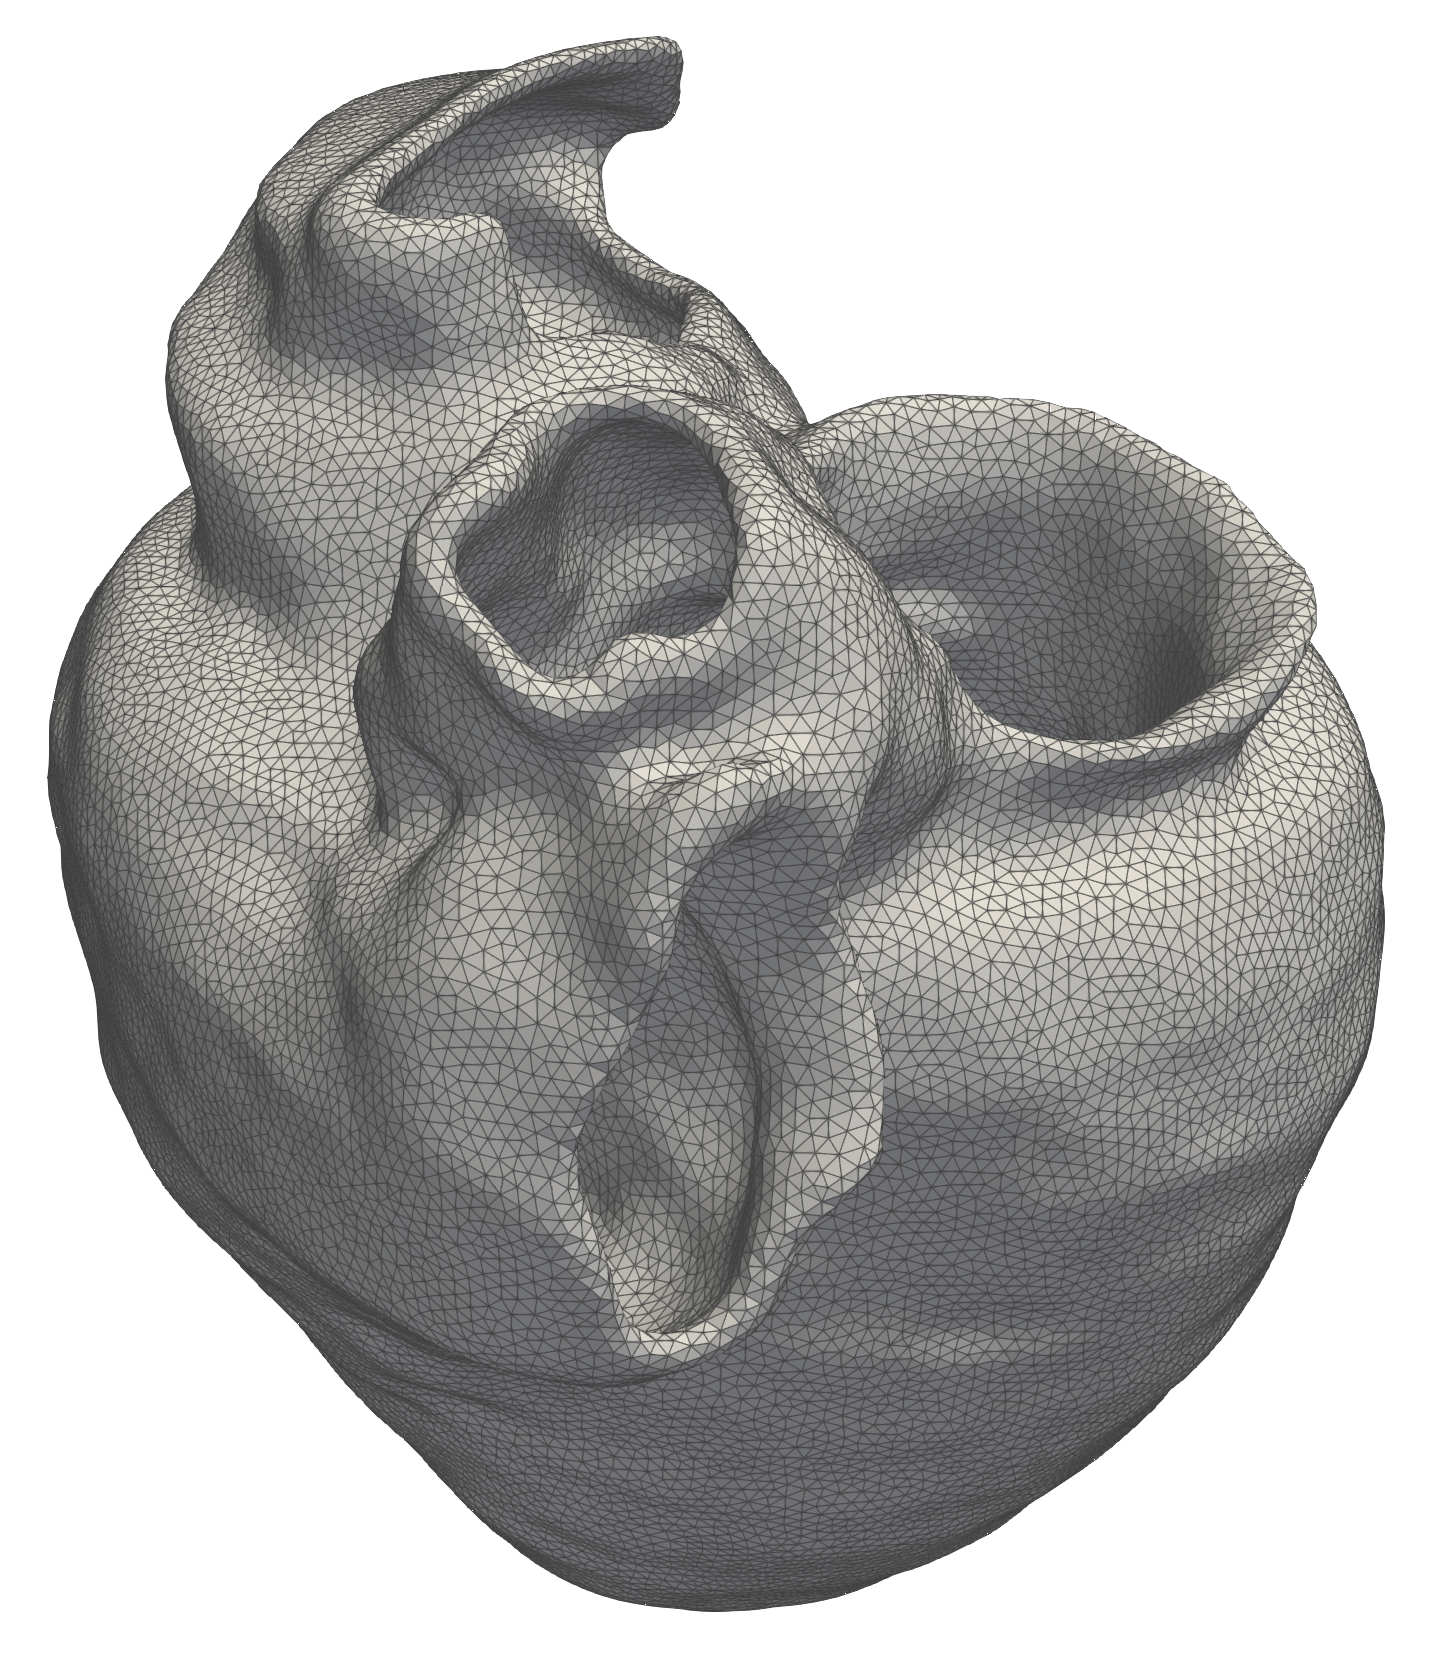
\includegraphics[scale=0.08]{media/2-shabaka/mesh.png}
\label{fig:shabakaseq5}}
%
\caption{(a) Segmented image, (b) point/normal placement, (c) oriented point cloud (normals not shown), c) cleaned surface mesh generated from Voronoi partition (edges not shown), and d) final decimated and smoothed surface.}
\label{fig:shabakaseq}
\end{figure}

%%%%%%%%%%%%%%%%%%%%%%%%%%%%%%%%%%%%%%%%%%%%%%%
%%%%%%%%%%%%%%%%%%%%%%%%%%%%%%%%%%%%%%%%%%%%%%%


\section{Performance Assessment}
%

The performance of the proposed method is assessed by comparing its results to those of a commercially available state-of-the-art software package. Performance is measured quantitatively for canonical image masks defined by spheres of various radii and locations, and qualitatively using a variety of real MRI and CT scans. \\ \\
%
We pursue a quantitative understanding of the performance of our method by considering a sphere of radius $R$ and center $\bm{C}$.  An image mask is defined by assigning a bit $v$ to the voxel with center at $\bm{v}$ as:
\begin{align} 
	v &=  \begin{cases}
		1, & \text{if}\ d \left(\bm{v},\bm{C}\right) \le R \\
		0, & \text{otherwise},
	\end{cases}
\end{align}
where $d(\cdot,\cdot)$ is the Euclidean distance. The background image is assumed to have a 256 $\times$ 256 $\times$ 256 voxel resolution. \\ \\
%
In order to quantify performance, two error metrics are defined: a {\em shape error} and a {\em volume error}. These metrics characterize the departure of the b-rep from the perfect sphere.  There are two sources of error~\cite{young_2008}: 1) error due to approximating the perfect sphere with a binary image mask, or the {\em image-based error}; and 2) error due to reconstructing the binary image mask with a facetized b-rep.  The latter can be thought of as dictating a method's ability to {\em converge to geometry}. The image mask defined above does not, of course, yield perfect image-based accuracy, but for these purposes, we will assume that the image-based error is negligible and will focus on the ability of the method to converge to geometry.\\ \\
%
The shape error measures the surface-normal deviation of our algorithm's end-result b-rep from the perfect sphere. The measure is constructed first by projecting each facet of the b-rep onto the exact sphere. The normal of each facet is compared to the normal of the exact sphere at the centroid of the projected facet by computing the magnitude of their cross product. An area-weighted sum is then taken over the b-rep, and finally the sum is normalized by the surface area of the b-rep. The error measure therefore lies in the range [0,1]. The shape error $e_s$, as described, can be calculated from:
\begin{equation} 
	e_s = \frac{ \sum \limits_{f\in\mathcal{F}} A_f \lVert {\bf n}_f \times {\bf n}_s \rVert}{\sum \limits_{f\in\mathcal{F}} A_f},
\end{equation}
where $A_f$ is the area and ${\bm n}_f$ is the unit normal of facet $f$, $\mathcal{F}$ is the set of all b-rep facets, and ${\bm n}_s$ is the normal of the exact sphere at the centroid of the projected facet $f$ onto the sphere. \\ \\
%
The volume error measures the unsigned volume enclosed between the b-rep and the exact sphere. We calculate this measure via a sum of integrals over the projections $\gamma_f$ of each facet onto the exact sphere: 
\begin{equation}
\label{vol err}
	e_v = \frac{1}{4\pi R^2} \Big[\sum \limits_{f \in \mathcal{F}\textsl{}} \ \int \limits_{\gamma_f} (r - R)^2 d\alpha \Big]^{1/2} .
\end{equation}
Here, $r = \lVert {\bm x} \rVert$ is the distance from the sphere center to a point on the planar facet associated with the projection $\gamma_f$, and $R$ is the radius of the exact sphere.  The indicated integrals are performed numerically on the projected facets. Six quadrature points were found to provide sufficient accuracy. The volume error is rendered dimensionless by normalizing by the surface area of the underlying perfect sphere.
\\ \\
%
The shape and volume errors were compared between the commercial software and the proposed method for a perfect sphere embedded in a fixed $256 \times 256 \times 256$ array of voxels.  In the comparisons presented below, three independent parameters were varied:  1) b-rep resolution, 2) sphere radius, and 3) sphere center location relative to the voxel array. The purpose of these comparisons is to show that the method performs comparably to an established option, rather than specifically pointing to the clear superiority of one method over the other. Optimal results were obtained from the commercial package by selecting the ``binarise before smoothing" option, and performing 100 iterations of ``smart mask smoothing''; standard options were chosen otherwise. \\ \\
%
\figref{graph1} shows the shape and volume errors for the two methods as the b-rep resolution is varied, for a spherical mask of radius $R = 80$ voxels centered in the image. See~\figref{demos1} for a visual comparison of the image mask with representative b-reps from the commercial code and the proposed method. Default parameters were used in the commercial code for b-reps with $n \ge 2587$ vertices. For resolutions coarser than that, the ``target maximum error" was increased to allow results with $n < 2587$. When comparing the shape error of the two approaches, the proposed method performs at least as well as the commercial option for coarse meshes ($n < 2500$), and performs measurably better -- up to $40\%$ improvement -- for finer b-reps ($n > 5000$). For the volume error, the proposed method performs up to $70\%$ better for b-reps with resolutions of $n < 5000$ vertices, and tends to a comparably small, but nonzero, value to which the commercial software converges.
\begin{figure}[h!]
\centering
\subfigure[]{%
	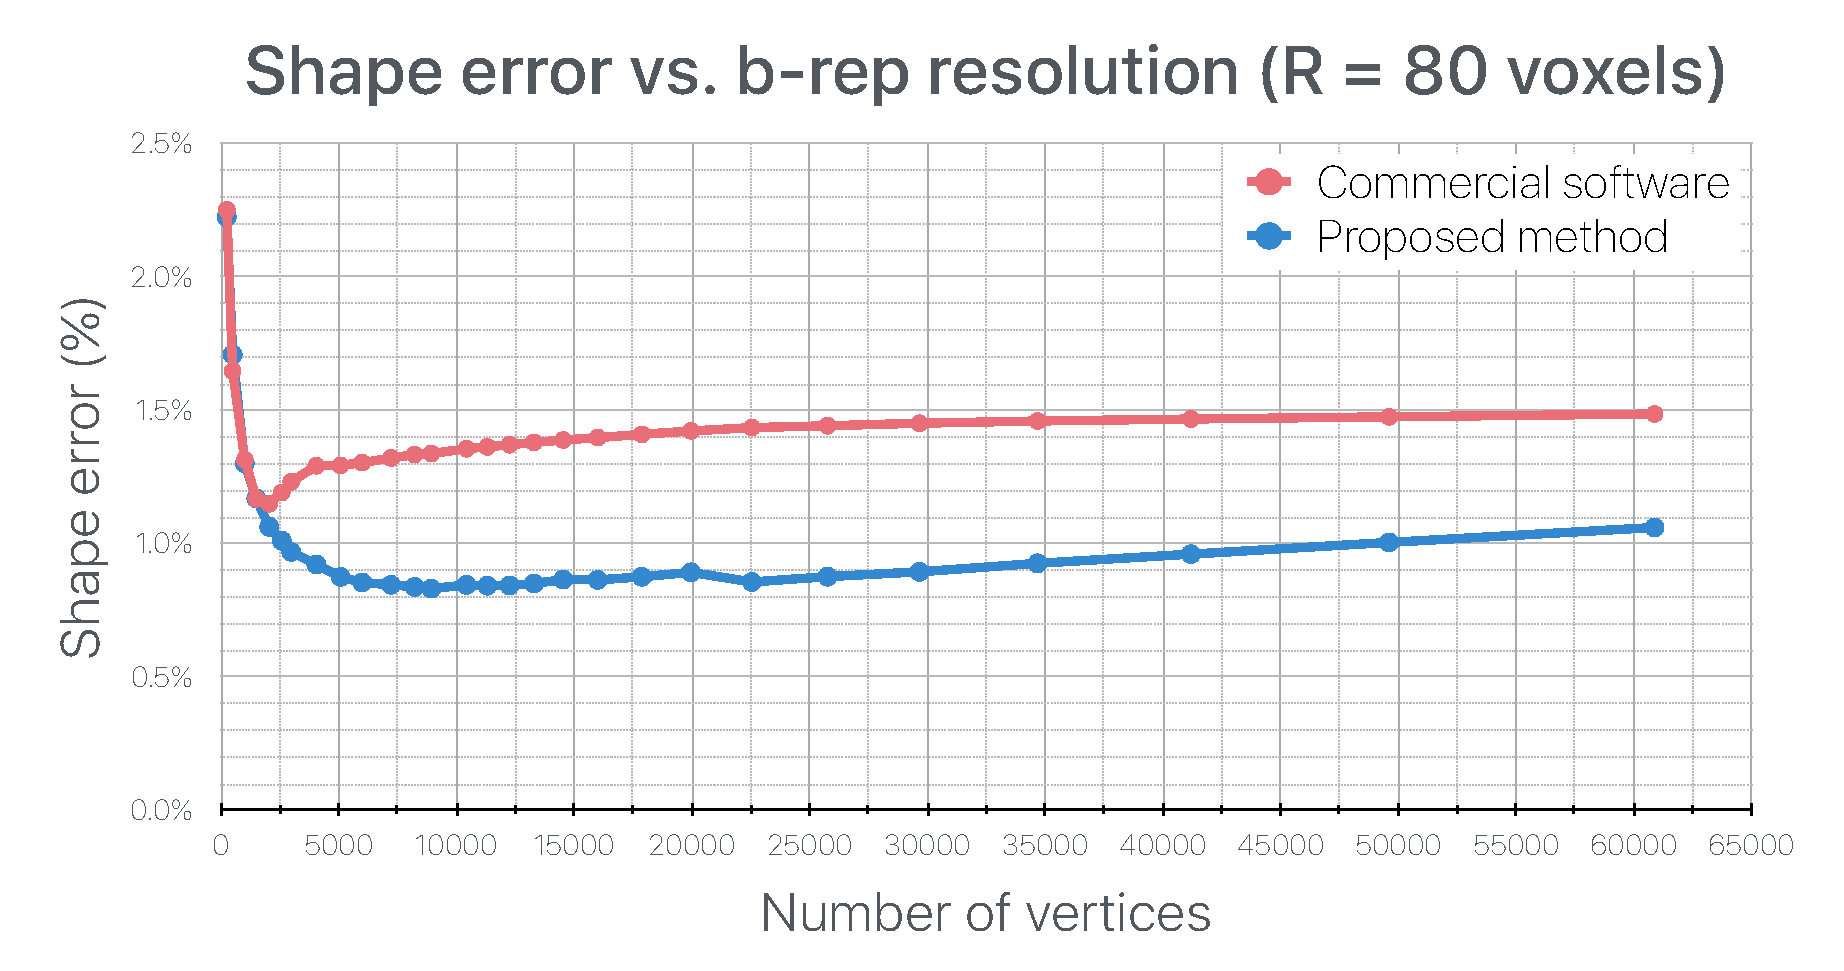
\includegraphics[scale=0.28]{media/7-performance/11-graph-1a.pdf}}
\subfigure[]{%
	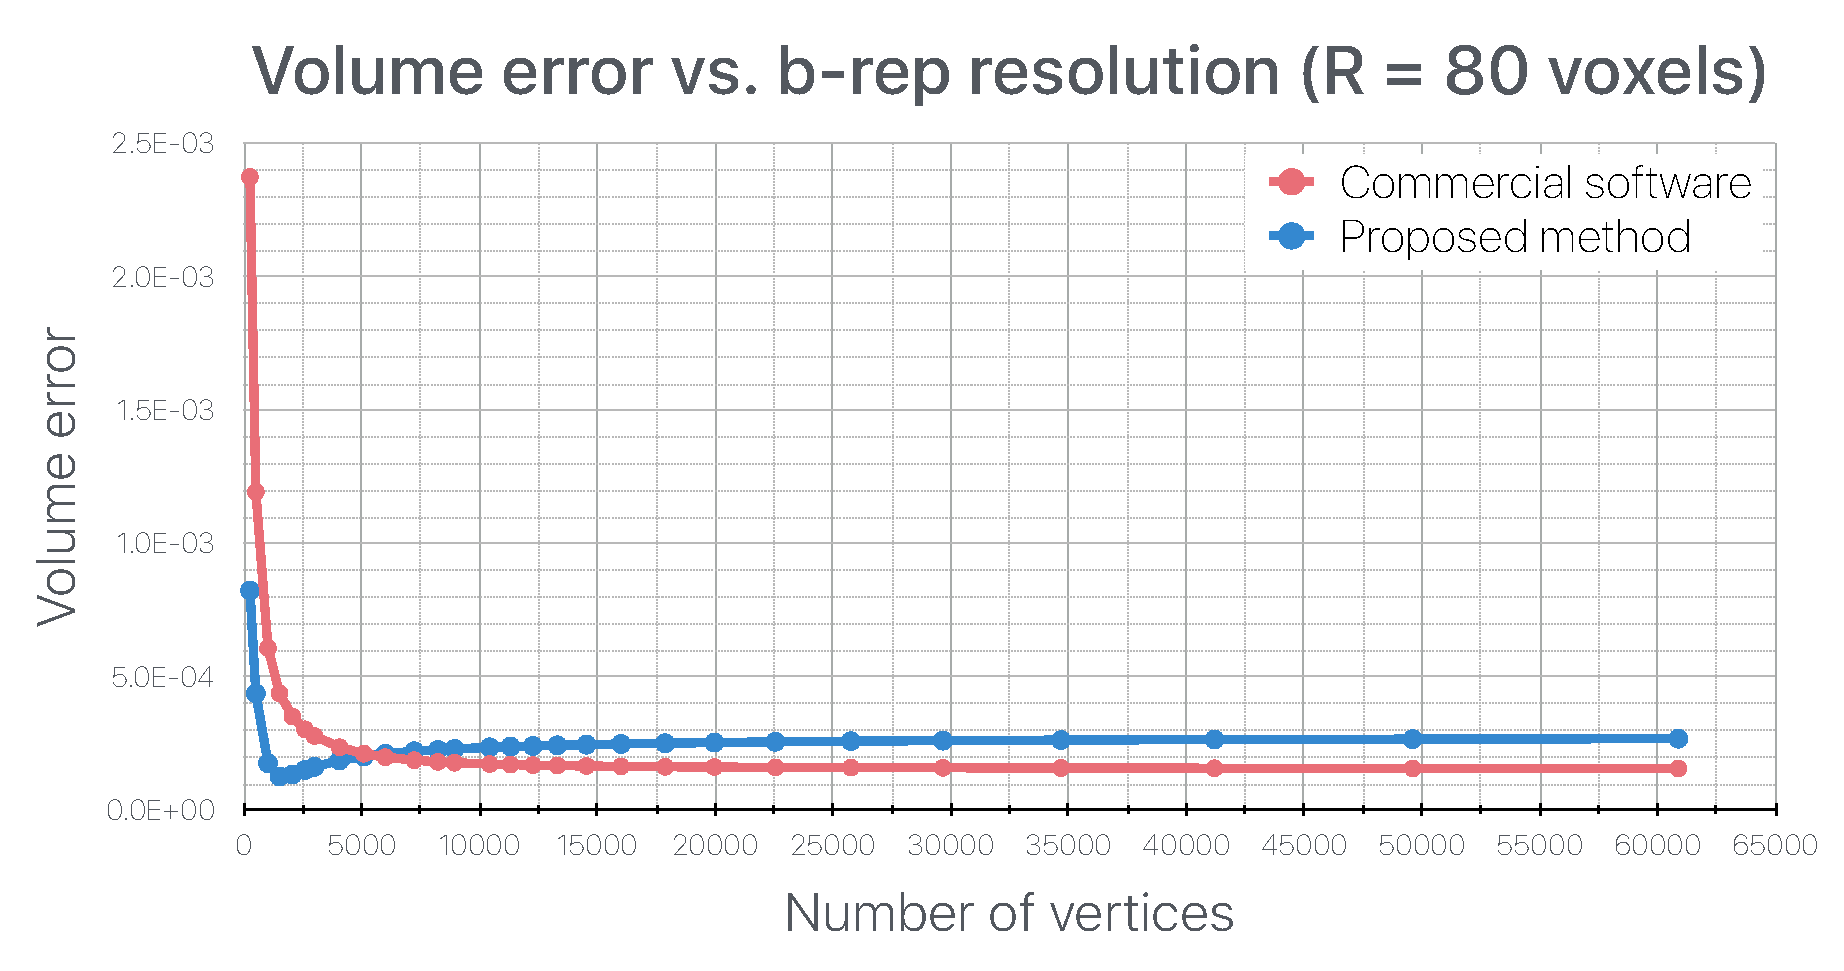
\includegraphics[scale=0.28]{media/7-performance/11-graph-1b.pdf}}
%	
\caption{Comparison of shape error (a) and volume error (b) between commercial software and proposed method as b-rep resolution is varied.}
\label{fig:graph1}
\end{figure}
\begin{figure}[ht!]
	\centering
	\includegraphics[scale=0.25]{media/7-performance/3-demos-4.pdf}
	\caption{Image masks (green) and corresponding b-reps for commercial software (red) and proposed method (blue) for selected b-rep resolutions.}
	\label{fig:demos1}
\end{figure} \\
%
\figref{graph2} shows the error metrics when the radius of the spherical mask is varied from 40 to 120 voxels, while keeping the sphere center fixed at the center of the image and the b-rep resolution fixed at $n = 10428$ vertices. See~\figref{demos2} for representative examples of the image mask and resulting b-reps from the two methods. The sphere radius represents an inverse measure of the curvature of the image mask relative to the voxel resolution; larger radii correspond to smoother surfaces. Both the shape and volume errors of the proposed method converge at roughly double the rate of the commercial approach's errors, with the proposed method's shape error the smaller of the two over the entire range of sphere radii considered.  In the case of the volume error, however, the proposed method's error is the greater over most of the range of radii, though it does converge at a faster rate. \\
\begin{figure}[b!]
	\centering
	\subfigure[]{%
		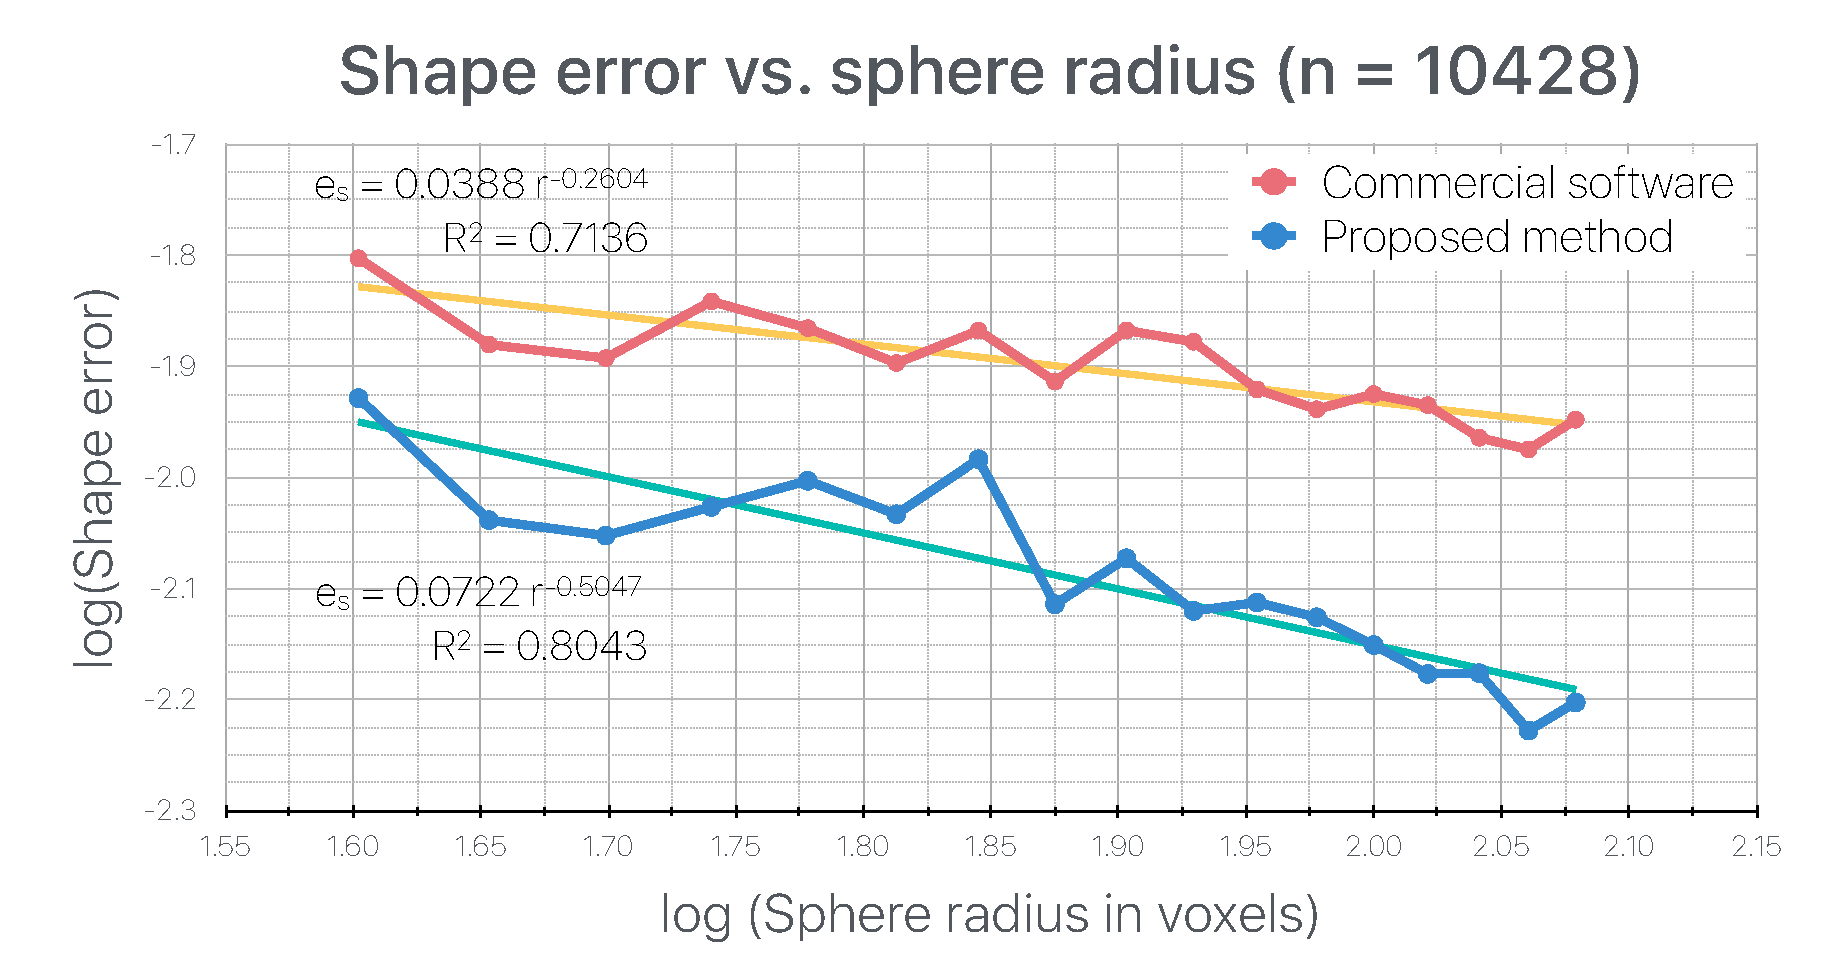
\includegraphics[scale=0.28]{media/7-performance/11-graph-2a.pdf}}
	\subfigure[]{%
		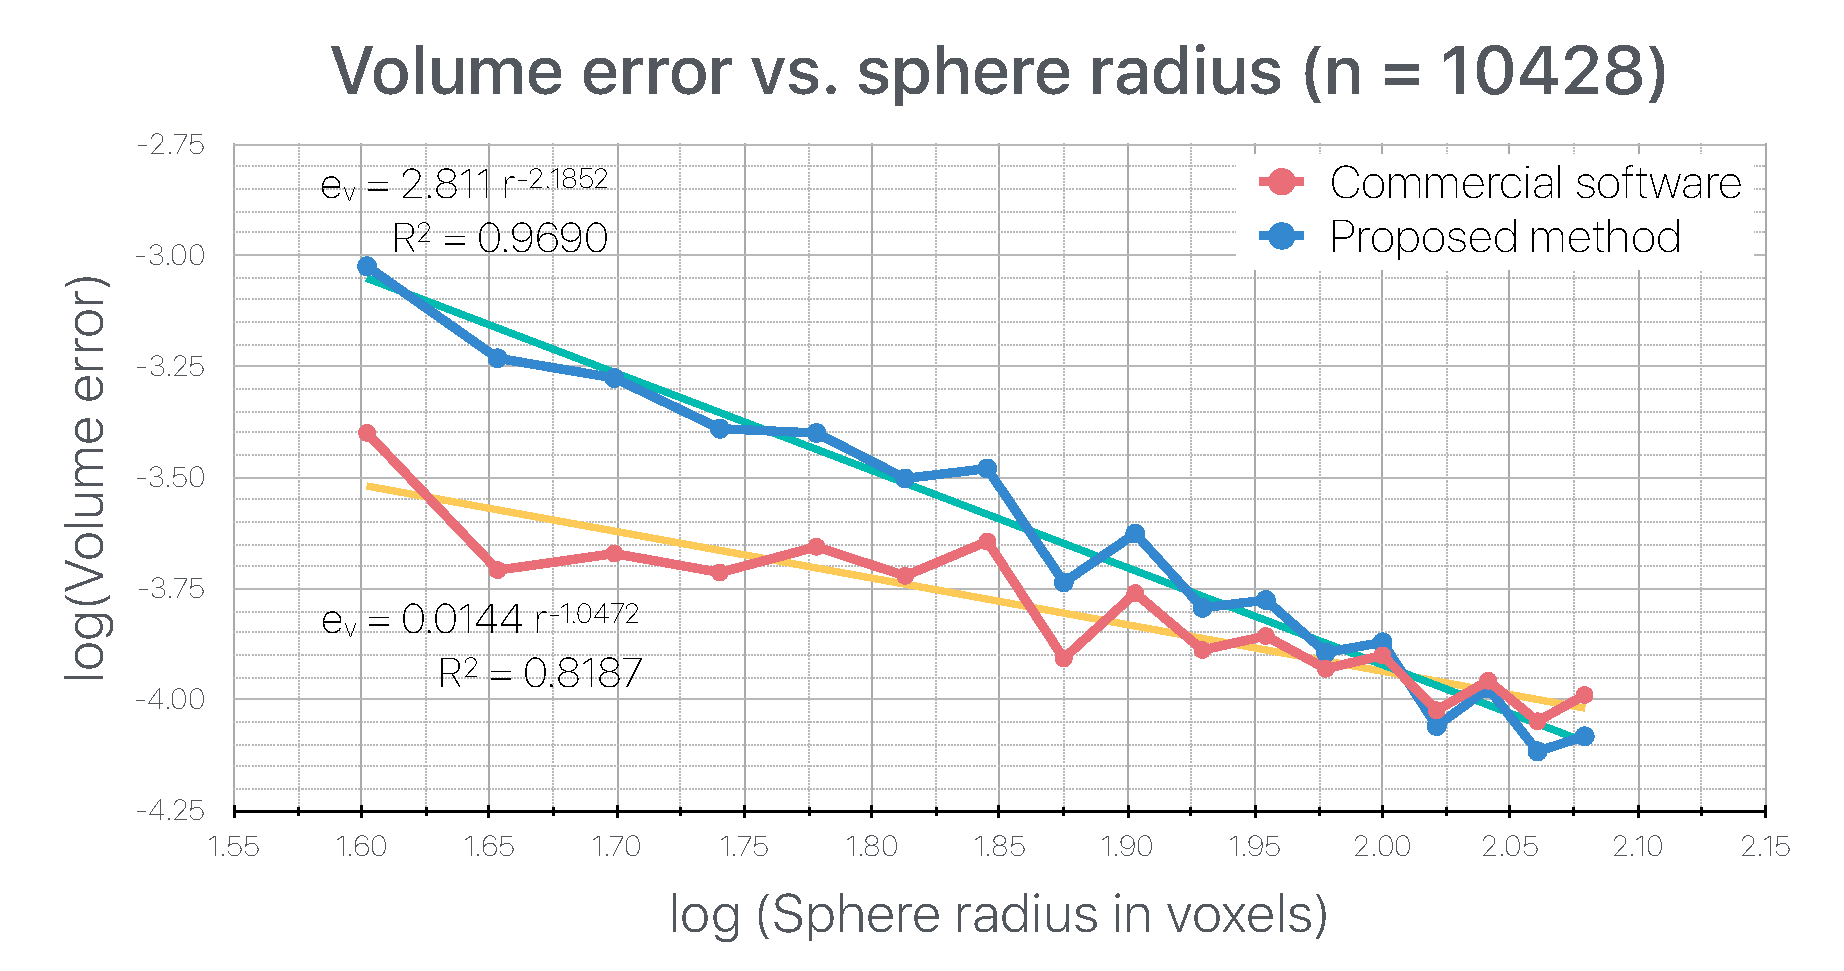
\includegraphics[scale=0.28]{media/7-performance/11-graph-2b.pdf}}
	%	
	\caption{Comparison of shape error (a) and volume error (b) between commercial software and proposed method as the radius of the exact sphere is varied.}
	\label{fig:graph2}
\end{figure}
\begin{figure}[ht!]
	\centering
	\includegraphics[scale=0.25]{media/7-performance/3-demos-5.pdf}
	\caption{Image masks (green) and corresponding b-reps for commercial software (red) and proposed method (blue) for selected sphere radii.}
	\label{fig:demos2}
\end{figure}
\noindent As a final point of quantitative comparison, the two methods are compared for a sphere of $R = 80$ voxels that is translated along the direction $\bm{i}  + 2\bm{j} + 3\bm{k}$, while keeping the resulting b-rep fixed at $n = 10428$ vertices. The intent of this case is to test the sensitivity of the methods to the location of the object relative to the image's voxel array. Ideally, the b-reps should be consistently accurate regardless of location.  Indeed, both methods show very low sensitivity to the translation of the object within the image, as shown in~\figref{graph3}. The relative standard deviations in the shape error for the commercial software and proposed method were $2.4\%$ and $1.1\%$, respectively, whereas for the volume error, they were $1.7\%$ and $2.1\%$, respectively. \\

\begin{figure}[b!]
	\centering
	\subfigure[]{%
		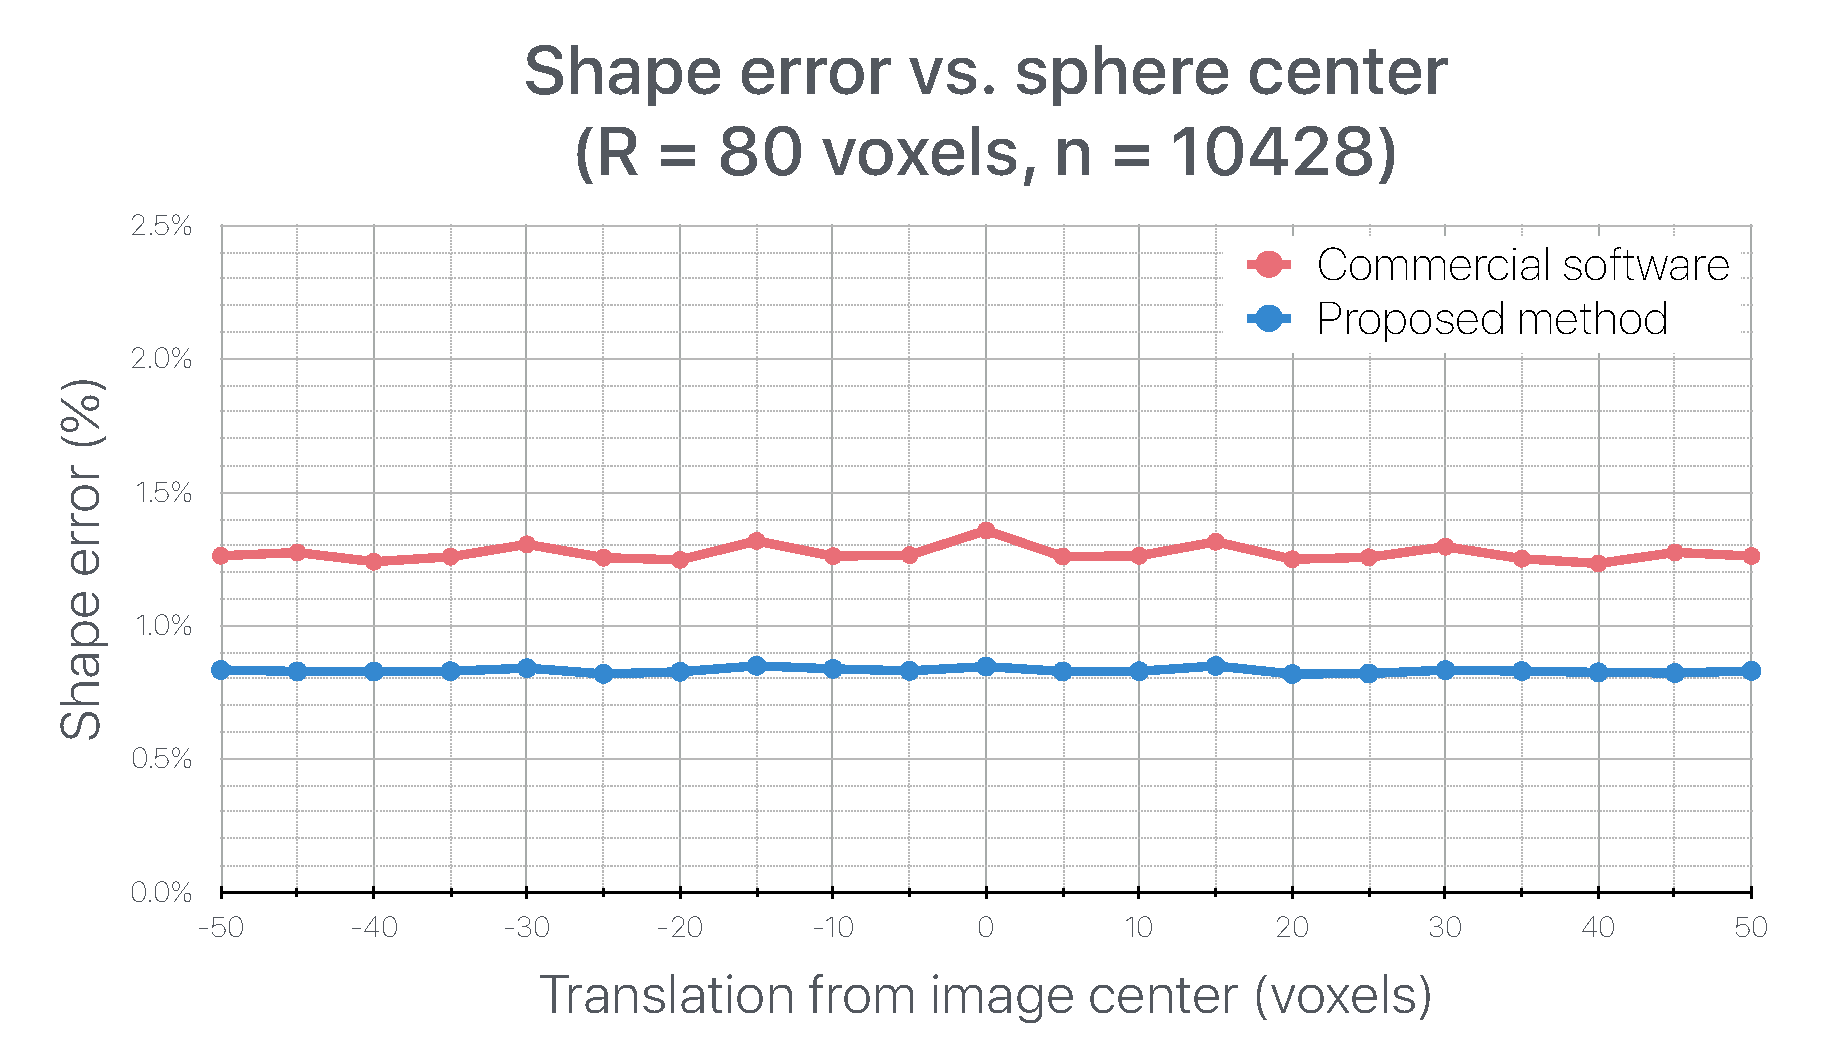
\includegraphics[scale=0.28]{media/7-performance/12-graph-3a.pdf}}
	\subfigure[]{%
		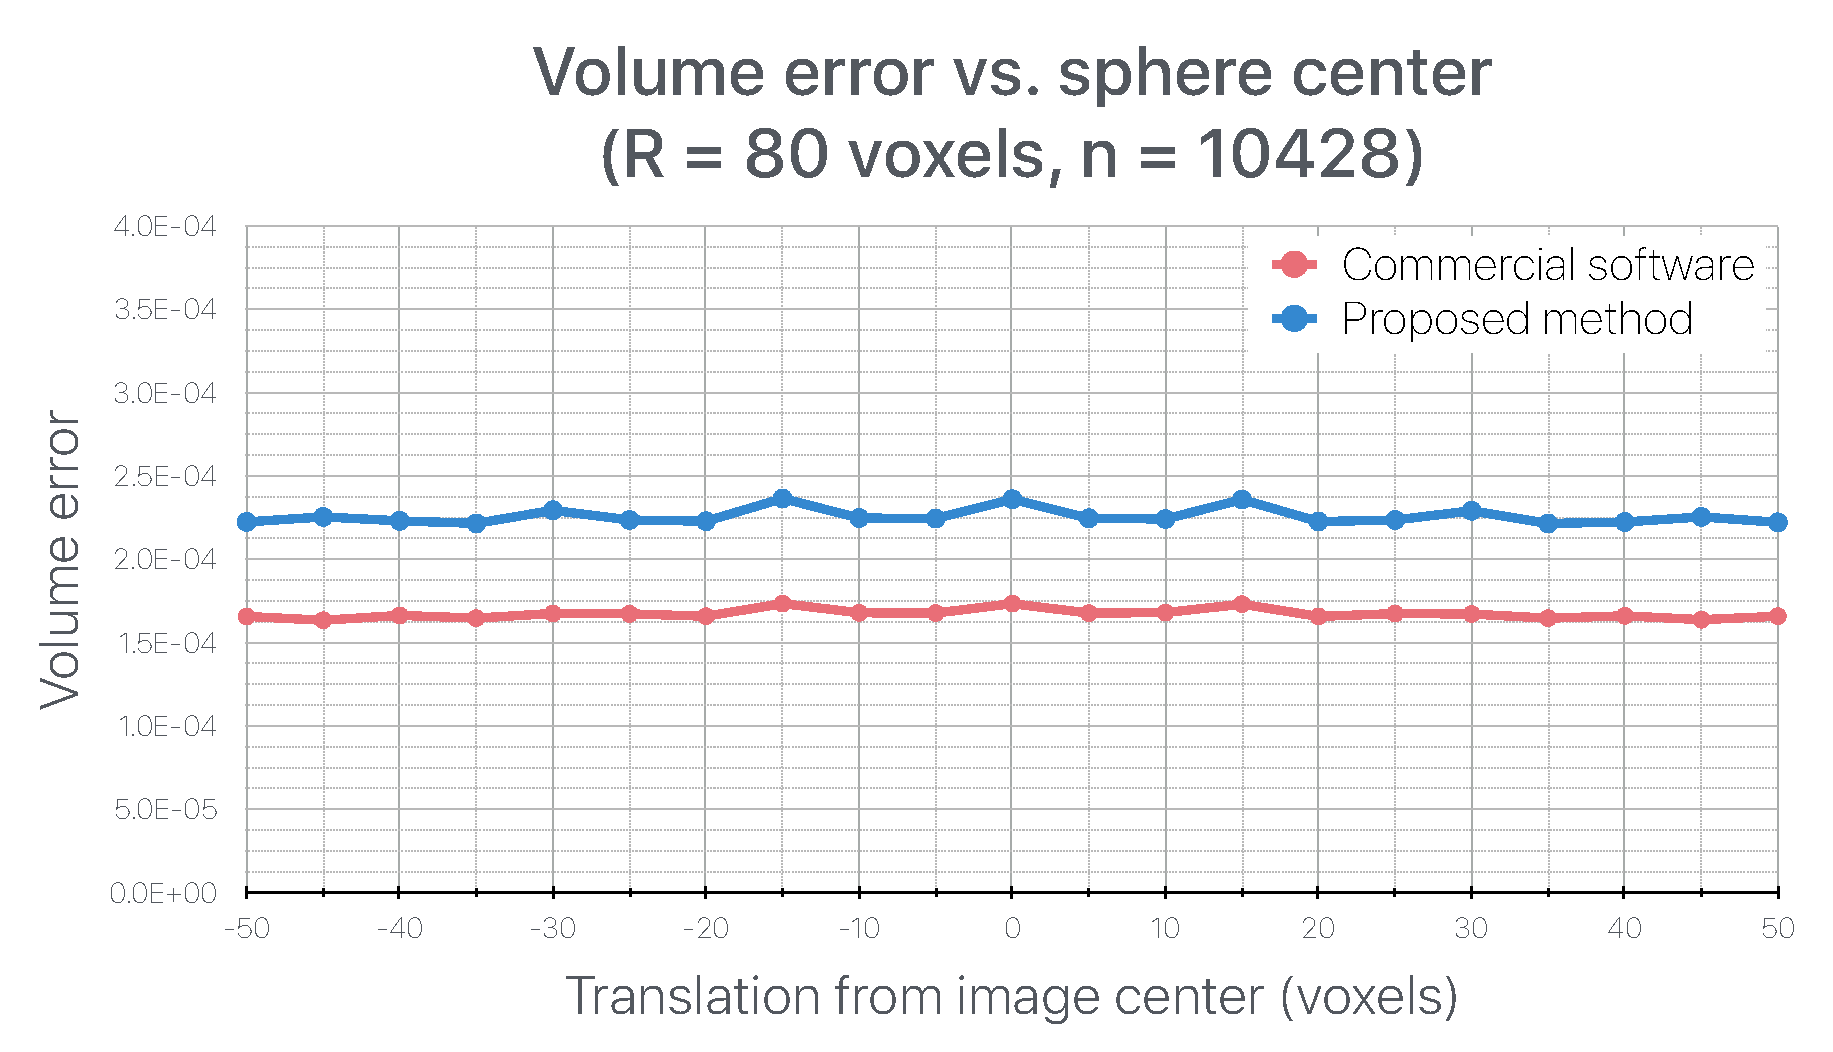
\includegraphics[scale=0.28]{media/7-performance/12-graph-3b.pdf}}
	%	
	\caption{Comparison of the shape error (a) and volume error (b) between the commercial software and the proposed method as the center of the sphere is translated relative to the image mask.}
	\label{fig:graph3}
\end{figure}

\noindent Lastly, we present several qualitative comparisons for real images generated by MRI and CT.  All images were segmented using \textit{Seg3D}~\cite{Seg3D}. The resulting binary image masks were used as input to the two methods. B-rep resolutions were matched between the two approaches in all cases, to make for a fair comparison. All examples completed for the proposed method on a 16 GB RAM laptop in less than 5 minutes. See~\figref{example-meshes} for comparisons of the image masks and resulting b-reps. Visual inspection suggests that the proposed method qualitatively performs comparably to the commercial approach in all cases, performing slightly better for smooth surfaces and not quite as well for regions with high curvature.  In this connection, we mention that the proposed method readily accommodates an enhancement that admits sharp edges and vertices (or corners), making the method particularly suitable for industrial applications involving manufactured objects.  Work on this enhancement is in progress.  The suite of examples presented here nonetheless illustrates a robustness and quality that demonstrate the proposed method as a viable approach.
\begin{figure}[h!]
	\centering
	\subfigure[]{%
		\includegraphics[scale=0.115]{media/7-performance/14-examples-a.pdf}}\hspace{1.2cm}
	\subfigure[]{%
		\includegraphics[scale=0.115]{media/7-performance/14-examples-b.pdf}}
	
	\subfigure[]{%
		\includegraphics[scale=0.115]{media/7-performance/14-examples-c.pdf}}\hspace{1.2cm}
	\subfigure[]{%
		\includegraphics[scale=0.115]{media/7-performance/14-examples-d.pdf}}
		
	\subfigure[]{%
		\includegraphics[scale=0.115]{media/7-performance/14-examples-e.pdf}}\hspace{1.2cm}
	\subfigure[]{%
		\includegraphics[scale=0.115]{media/7-performance/14-examples-f.pdf}}
		
	\subfigure[]{%
		\includegraphics[scale=0.115]{media/7-performance/14-examples-g.pdf}}\hspace{1.2cm}
	\subfigure[]{%
		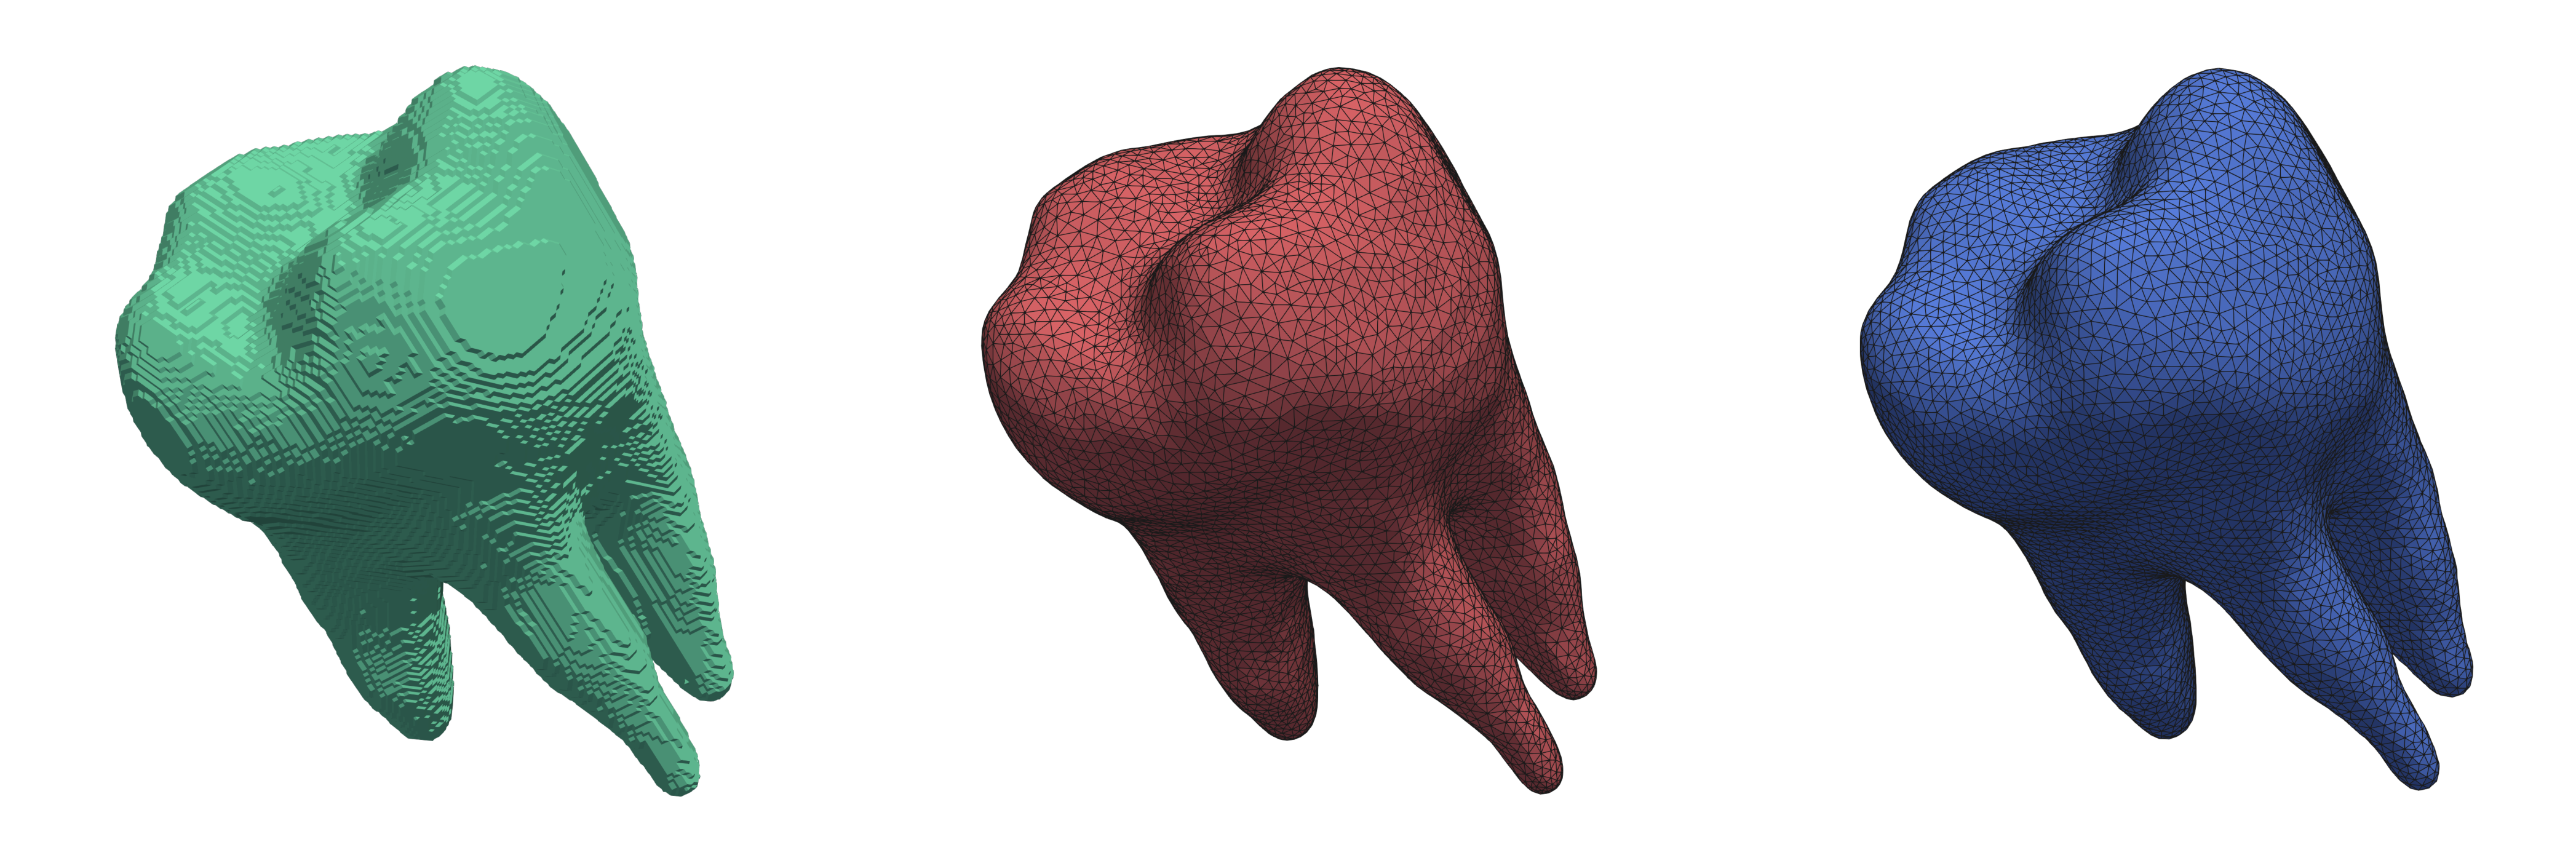
\includegraphics[scale=0.115]{media/7-performance/14-examples-h.pdf}}
	
	\subfigure[]{%
		\includegraphics[scale=0.115]{media/7-performance/14-examples-i.pdf}}\hspace{1.2cm}
	\subfigure[]{%
		\includegraphics[scale=0.115]{media/7-performance/14-examples-j.pdf}}
	\caption{Image masks (green) and corresponding b-reps for commercial software (red) and proposed method (blue) for various examples from MRI and CT: (a) brain~\cite{marcus_2007}, (b) heart~\cite{cvgg}, (c) lungs~\cite{rikxoort_2009}, (d) distal femur~\cite{epperson_2013}, (e) skull~\cite{clark_2013}, (f) L5 lumbar~\cite{yao_2016}, (g) pelvis~\cite{clark_2013}, (h) upper left second molar (author's), (i) liver~\cite{bilic_2019}, and (j) example image with disjoint objects in image mask.}
	\label{fig:example-meshes}
\end{figure}
\section{{Limitations and Future Extensions}}

IGNORE
\section{Closure}

We propose a workflow for creation of a watertight, manifold, facetized boundary representation given a binary image mask containing noise.  Our target application is physics-based simulation, for which a volume mesh must of course be generated by separate means (e.g. tetrahedral advancing-front generator).  The method densely samples the image mask and locally approximates the interface between neighboring materials based on a local template surface. The optimal orientation of the template surface is obtained via minimization of a weighted error function. The error function is based on the difference in the zeroth, first, and second polynomial moments of the voxelated sampling window and the region created by the approximating template. Oriented points are then placed with the help of each optimal local surface. In aggregate, the local templates produce an oriented point cloud whose density is controlled by the selected window-size and window-overlap parameters.  This procedure provides for effective smoothing of the surface normal while retaining the surface ``position'' data inherent in the image mask.  The oriented-point-cloud procedure does not assume the existence of a target surface with the desired topology.  Instead, it in effect synthesizes a surface that ignores fine-scale islands and holes in the image mask, as often occur in noisy segmented images.  This is an important distinguishing feature of our method.

With the oriented point cloud in hand, the method utilizes Voronoi partitioning as a means of performing surface reconstruction from the point cloud.  Specifically, Voronoi sites are placed on either side of each point along its normal vector, and material identifiers (or colors) are assigned to the sites. A Voronoi partition of 3D space is performed, and the b-rep is extracted in the form of the complex of facets that share Voronoi sites of differing material ID. This technique takes advantage of some useful properties of the Voronoi tessellation, including being guaranteed manifold. Following construction of the Voronoi surface, decimation and smoothing are performed.  Comparisons to three other workflows show that the proposed approach performs competitively with respect to shape and volume of analytic spherical surfaces. The approach was also seen to perform well for a variety of examples from real MRI and CT scans.

With the current framework established in its basic form, work has turned to extending the method to geometries with sharp corners or edges, high-curvature regions, and multiple materials.  The extension to sharp features is accomplished through introduction of new local-interface templates to supplement the simple planar one used herein.  Specifically, an edge template would allow for the introduction of three Voronoi sites, and a corner template would produce four. These enhancements hold the promise of generating b-reps that naturally capture surfaces with sharp edges and corners, even when coarse windowing is selected in the point-cloud-generation step.  It is largely with these properties in mind that we chose a Voronoi-based approach for the surface-reconstruction step, rather than e.g. a Delaunay-based one.   More generally, templates can be designed with multiple oriented points, such that high local curvature can be obtained where dictated by the image mask.  

A limitation of our method at its present stage of development is that it is limited to binary images.  While the Voronoi-based surface-reconstruction technique is readily adaptable to the multi-material case, the window-based point-cloud step would require more work.  Specifically, new and probably complex local-interface templates would have to be introduced.  While there are no theoretical constraints that would prevent this, the practicalities have yet to be explored.
\section*{Acknowledgments}

Financial support from DOE CSGF grant DE-FG02-97ER25308 is gratefully acknowledged.
The authors would also like to express their appreciation to the two anonymous
reviewers for their particularly insightful and valuable comments.

%%%%%%%%%%%%%%%%%%%%%%%%%%%%%%%%%%%%%%%%%%%%%%%%%%%%%%%%%%%%%%%%%%%%%%%%

\printbibliography
% HERE
% \bibliography{references}
% HERE

%%%%%%%%%%%%%%%%%%%%%%%%%%%%%%%%%%%%%%%%%%%%%%%%%%%%%%%%%%%%%%%%%%%%%%%%

\end{document}
